\documentclass[a4paper,12pt]{report}

\usepackage[utf8]{inputenc}
\usepackage[T1]{fontenc}
\usepackage{array}
\usepackage{amsmath}
\usepackage[english]{babel}
\usepackage{graphicx}
\usepackage[a4paper]{geometry}
\usepackage[colorlinks=true,urlcolor=blue,linkcolor=blue]{hyperref}
\usepackage{url}
\usepackage[nottoc,numbib]{tocbibind}
\usepackage{color}
\usepackage{epstopdf}
\usepackage{xcolor}
\usepackage{rotating}

\makeatletter
	\renewcommand{\thechapter}{\Roman{chapter}}
\makeatother

\begin{document}

\chapter{Diluted magnetic semiconductor quantum dots\label{DMSQDTh}}

	\section{II-VI semiconductor quantum dots}
	
		\subsection{Band structure of CdTe/ZnTe\label{BandStruct}}
		
		Lorem ipsum dolor sit amet, consectetur adipiscing elit. Curabitur tortor quam, imperdiet quis facilisis sed, fringilla a quam. Cras ante odio, hendrerit ac ante nec, cursus imperdiet urna. Mauris convallis ultricies purus, nec condimentum erat bibendum vel. Aliquam erat volutpat. Pellentesque condimentum, eros a consequat accumsan, turpis sem euismod nisi, sed fringilla quam turpis sit amet erat. Mauris dictum odio sed nisi dapibus, et molestie mauris rutrum. Praesent convallis dolor in nibh blandit bibendum. Quisque sit amet arcu consectetur lorem luctus venenatis nec quis dui. Aliquam erat volutpat. Aenean auctor elit nec tristique dignissim. Nulla massa mi, efficitur semper ex id, pretium eleifend massa. Vivamus sit amet orci scelerisque, gravida est ut, vulputate odio.
		
	\begin{figure}[h!]
	\begin{center}
		\includegraphics[width=10cm]{FillingPicture.png}
	\end{center}
	\caption{Zinc-blende crystal structure and first Brillouin zone.}
	\label{Zinc-Blende&Brillouin}
	\end{figure}

	Curabitur eget ipsum egestas dui viverra suscipit. Cras aliquet lacus vitae erat finibus semper. Nulla pharetra eget urna vitae sodales. Nunc faucibus velit lacus, nec ornare eros aliquet quis. Donec a orci nec sem pulvinar ultricies sit amet ut arcu. Nullam id vehicula enim, at tincidunt velit. Duis vestibulum lorem a molestie fringilla. Nullam tincidunt semper placerat. Donec nibh sem, ornare eget cursus ac, luctus sit amet eros. Phasellus eget interdum nisi. Donec mollis risus id lectus fringilla, et commodo risus iaculis. Donec at lacus sed nibh posuere posuere sit amet eget sapien. In dignissim, enim sit amet convallis fermentum, lacus nulla gravida tortor, non facilisis ex nisl sit amet augue. Maecenas eu enim condimentum, consectetur ligula vel, tincidunt nisl. Nam laoreet dictum volutpat. Donec at erat venenatis, ultrices lorem ac, vestibulum neque.

	\begin{figure}[h!]
	\begin{center}
		\includegraphics[width=10cm]{FillingPicture.png}
	\end{center}
	\caption{CdTe/ZnTe band structures}
	\label{BandStruct}
	\end{figure}
		
		\subsection{Lattice mismatch and the Bir-Pikus Hamiltonian}
		
		Lorem ipsum dolor sit amet, consectetur adipiscing elit. Curabitur tortor quam, imperdiet quis facilisis sed, fringilla a quam. Cras ante odio, hendrerit ac ante nec, cursus imperdiet urna. Mauris convallis ultricies purus, nec condimentum erat bibendum vel. Aliquam erat volutpat. Pellentesque condimentum, eros a consequat accumsan, turpis sem euismod nisi, sed fringilla quam turpis sit amet erat. Mauris dictum odio sed nisi dapibus, et molestie mauris rutrum. Praesent convallis dolor in nibh blandit bibendum. Quisque sit amet arcu consectetur lorem luctus venenatis nec quis dui. Aliquam erat volutpat. Aenean auctor elit nec tristique dignissim. Nulla massa mi, efficitur semper ex id, pretium eleifend massa. Vivamus sit amet orci scelerisque, gravida est ut, vulputate odio.

	Curabitur eget ipsum egestas dui viverra suscipit. Cras aliquet lacus vitae erat finibus semper. Nulla pharetra eget urna vitae sodales. Nunc faucibus velit lacus, nec ornare eros aliquet quis. Donec a orci nec sem pulvinar ultricies sit amet ut arcu. Nullam id vehicula enim, at tincidunt velit. Duis vestibulum lorem a molestie fringilla. Nullam tincidunt semper placerat. Donec nibh sem, ornare eget cursus ac, luctus sit amet eros. Phasellus eget interdum nisi. Donec mollis risus id lectus fringilla, et commodo risus iaculis. Donec at lacus sed nibh posuere posuere sit amet eget sapien. In dignissim, enim sit amet convallis fermentum, lacus nulla gravida tortor, non facilisis ex nisl sit amet augue. Maecenas eu enim condimentum, consectetur ligula vel, tincidunt nisl. Nam laoreet dictum volutpat. Donec at erat venenatis, ultrices lorem ac, vestibulum neque. 
		
		\subsection{Valence band mixing}	
		
		Lorem ipsum dolor sit amet, consectetur adipiscing elit. Curabitur tortor quam, imperdiet quis facilisis sed, fringilla a quam. Cras ante odio, hendrerit ac ante nec, cursus imperdiet urna. Mauris convallis ultricies purus, nec condimentum erat bibendum vel. Aliquam erat volutpat. Pellentesque condimentum, eros a consequat accumsan, turpis sem euismod nisi, sed fringilla quam turpis sit amet erat. Mauris dictum odio sed nisi dapibus, et molestie mauris rutrum. Praesent convallis dolor in nibh blandit bibendum. Quisque sit amet arcu consectetur lorem luctus venenatis nec quis dui. Aliquam erat volutpat. Aenean auctor elit nec tristique dignissim. Nulla massa mi, efficitur semper ex id, pretium eleifend massa. Vivamus sit amet orci scelerisque, gravida est ut, vulputate odio.

	Curabitur eget ipsum egestas dui viverra suscipit. Cras aliquet lacus vitae erat finibus semper. Nulla pharetra eget urna vitae sodales. Nunc faucibus velit lacus, nec ornare eros aliquet quis. Donec a orci nec sem pulvinar ultricies sit amet ut arcu. Nullam id vehicula enim, at tincidunt velit. Duis vestibulum lorem a molestie fringilla. Nullam tincidunt semper placerat. Donec nibh sem, ornare eget cursus ac, luctus sit amet eros. Phasellus eget interdum nisi. Donec mollis risus id lectus fringilla, et commodo risus iaculis. Donec at lacus sed nibh posuere posuere sit amet eget sapien. In dignissim, enim sit amet convallis fermentum, lacus nulla gravida tortor, non facilisis ex nisl sit amet augue. Maecenas eu enim condimentum, consectetur ligula vel, tincidunt nisl. Nam laoreet dictum volutpat. Donec at erat venenatis, ultrices lorem ac, vestibulum neque. 
		
		\subsection{Electron-hole interaction in confined structure\label{e-hIntQD}}
		
		Lorem ipsum dolor sit amet, consectetur adipiscing elit. Curabitur tortor quam, imperdiet quis facilisis sed, fringilla a quam. Cras ante odio, hendrerit ac ante nec, cursus imperdiet urna. Mauris convallis ultricies purus, nec condimentum erat bibendum vel. Aliquam erat volutpat. Pellentesque condimentum, eros a consequat accumsan, turpis sem euismod nisi, sed fringilla quam turpis sit amet erat. Mauris dictum odio sed nisi dapibus, et molestie mauris rutrum. Praesent convallis dolor in nibh blandit bibendum. Quisque sit amet arcu consectetur lorem luctus venenatis nec quis dui. Aliquam erat volutpat. Aenean auctor elit nec tristique dignissim. Nulla massa mi, efficitur semper ex id, pretium eleifend massa. Vivamus sit amet orci scelerisque, gravida est ut, vulputate odio.
		
	\begin{figure}[h!]
	\begin{center}
		\includegraphics[width=10cm]{FillingPicture.png}
	\end{center}
	\caption{Dots STM images}
	\label{STM}
	\end{figure}

	Curabitur eget ipsum egestas dui viverra suscipit. Cras aliquet lacus vitae erat finibus semper. Nulla pharetra eget urna vitae sodales. Nunc faucibus velit lacus, nec ornare eros aliquet quis. Donec a orci nec sem pulvinar ultricies sit amet ut arcu. Nullam id vehicula enim, at tincidunt velit. Duis vestibulum lorem a molestie fringilla. Nullam tincidunt semper placerat. Donec nibh sem, ornare eget cursus ac, luctus sit amet eros. Phasellus eget interdum nisi. Donec mollis risus id lectus fringilla, et commodo risus iaculis. Donec at lacus sed nibh posuere posuere sit amet eget sapien. In dignissim, enim sit amet convallis fermentum, lacus nulla gravida tortor, non facilisis ex nisl sit amet augue. Maecenas eu enim condimentum, consectetur ligula vel, tincidunt nisl. Nam laoreet dictum volutpat. Donec at erat venenatis, ultrices lorem ac, vestibulum neque.
	
	
	\section{Fine and hyperfine structure of a magnetic atom in II-VI semiconductor}
	
		\subsection{Mn atom in II-VI semiconductor}

		Mn in a lattice -> modification of orbital -> spin-orbit interaction. Magnetic anisotropy + anisotropy of strain. (Mn has nuclear spin 5/2 -> hyperfine interaction?)

	\begin{figure}[h!]
	\begin{center}
		\includegraphics[width=10cm]{FillingPicture.png}
	\end{center}
	\caption{Mn in Zinc-Blend lattice}
	\label{MnInclusion}
	\end{figure}
		
		Lorem ipsum dolor sit amet, consectetur adipiscing elit. Curabitur tortor quam, imperdiet quis facilisis sed, fringilla a quam. Cras ante odio, hendrerit ac ante nec, cursus imperdiet urna. Mauris convallis ultricies purus, nec condimentum erat bibendum vel. Aliquam erat volutpat. Pellentesque condimentum, eros a consequat accumsan, turpis sem euismod nisi, sed fringilla quam turpis sit amet erat. Mauris dictum odio sed nisi dapibus, et molestie mauris rutrum. Praesent convallis dolor in nibh blandit bibendum. Quisque sit amet arcu consectetur lorem luctus venenatis nec quis dui. Aliquam erat volutpat. Aenean auctor elit nec tristique dignissim. Nulla massa mi, efficitur semper ex id, pretium eleifend massa. Vivamus sit amet orci scelerisque, gravida est ut, vulputate odio.

	\begin{figure}[h!]
	\begin{center}
		\includegraphics[width=10cm]{FillingPicture.png}
	\end{center}
	\caption{Mn fine and hyperfine structure}
	\label{MnFineHyperfines}
	\end{figure}

	Curabitur eget ipsum egestas dui viverra suscipit. Cras aliquet lacus vitae erat finibus semper. Nulla pharetra eget urna vitae sodales. Nunc faucibus velit lacus, nec ornare eros aliquet quis. Donec a orci nec sem pulvinar ultricies sit amet ut arcu. Nullam id vehicula enim, at tincidunt velit. Duis vestibulum lorem a molestie fringilla. Nullam tincidunt semper placerat. Donec nibh sem, ornare eget cursus ac, luctus sit amet eros. Phasellus eget interdum nisi. Donec mollis risus id lectus fringilla, et commodo risus iaculis. Donec at lacus sed nibh posuere posuere sit amet eget sapien. In dignissim, enim sit amet convallis fermentum, lacus nulla gravida tortor, non facilisis ex nisl sit amet augue. Maecenas eu enim condimentum, consectetur ligula vel, tincidunt nisl. Nam laoreet dictum volutpat. Donec at erat venenatis, ultrices lorem ac, vestibulum neque.
	
		\subsection{Cr atom in II-VI semiconductor\label{CrSemiCon}}

	\begin{figure}[h!]
	\begin{center}
		\includegraphics[width=10cm]{FillingPicture.png}
	\end{center}
	\caption{Cr in Zinc-Blend lattice}
	\label{CrInclusion}
	\end{figure}
	
		Lorem ipsum dolor sit amet, consectetur adipiscing elit. Curabitur tortor quam, imperdiet quis facilisis sed, fringilla a quam. Cras ante odio, hendrerit ac ante nec, cursus imperdiet urna. Mauris convallis ultricies purus, nec condimentum erat bibendum vel. Aliquam erat volutpat. Pellentesque condimentum, eros a consequat accumsan, turpis sem euismod nisi, sed fringilla quam turpis sit amet erat. Mauris dictum odio sed nisi dapibus, et molestie mauris rutrum. Praesent convallis dolor in nibh blandit bibendum. Quisque sit amet arcu consectetur lorem luctus venenatis nec quis dui. Aliquam erat volutpat. Aenean auctor elit nec tristique dignissim. Nulla massa mi, efficitur semper ex id, pretium eleifend massa. Vivamus sit amet orci scelerisque, gravida est ut, vulputate odio.

	\begin{figure}[h!]
	\begin{center}
		\includegraphics[width=10cm]{FillingPicture.png}
	\end{center}
	\caption{Atomic configuration in Jahn-Teller effect + three minima}
	\label{Jahn-Teller}
	\end{figure}

	\begin{figure}[h!]
	\begin{center}
		\includegraphics[width=10cm]{FillingPicture.png}
	\end{center}
	\caption{Degeneracy breaking under Jahn-Teller effect}
	\label{DegenBreakJT}
	\end{figure}

	Curabitur eget ipsum egestas dui viverra suscipit. Cras aliquet lacus vitae erat finibus semper. Nulla pharetra eget urna vitae sodales. Nunc faucibus velit lacus, nec ornare eros aliquet quis. Donec a orci nec sem pulvinar ultricies sit amet ut arcu. Nullam id vehicula enim, at tincidunt velit. Duis vestibulum lorem a molestie fringilla. Nullam tincidunt semper placerat. Donec nibh sem, ornare eget cursus ac, luctus sit amet eros. Phasellus eget interdum nisi. Donec mollis risus id lectus fringilla, et commodo risus iaculis. Donec at lacus sed nibh posuere posuere sit amet eget sapien. In dignissim, enim sit amet convallis fermentum, lacus nulla gravida tortor, non facilisis ex nisl sit amet augue. Maecenas eu enim condimentum, consectetur ligula vel, tincidunt nisl. Nam laoreet dictum volutpat. Donec at erat venenatis, ultrices lorem ac, vestibulum neque.

	\begin{figure}[h!]
	\begin{center}
		\includegraphics[width=10cm]{FillingPicture.png}
	\end{center}
	\caption{Strain effect on ground state + degeneracy breaking by this symetry reduction}
	\label{StrainGS}
	\end{figure}

	\begin{figure}[h!]
	\begin{center}
		\includegraphics[width=10cm]{FillingPicture.png}
	\end{center}
	\caption{Overall energy structure (with +/- 2 which doesn't luminesce)}
	\label{EnerStruct}
	\end{figure}
	

	\section{Exchange interaction between carrier and magnetic atom}
	
		\subsection{Exchange interaction in Diluted Magnetic Semiconductors}
		
		Lorem ipsum dolor sit amet, consectetur adipiscing elit. Curabitur tortor quam, imperdiet quis facilisis sed, fringilla a quam. Cras ante odio, hendrerit ac ante nec, cursus imperdiet urna. Mauris convallis ultricies purus, nec condimentum erat bibendum vel. Aliquam erat volutpat. Pellentesque condimentum, eros a consequat accumsan, turpis sem euismod nisi, sed fringilla quam turpis sit amet erat. Mauris dictum odio sed nisi dapibus, et molestie mauris rutrum. Praesent convallis dolor in nibh blandit bibendum. Quisque sit amet arcu consectetur lorem luctus venenatis nec quis dui. Aliquam erat volutpat. Aenean auctor elit nec tristique dignissim. Nulla massa mi, efficitur semper ex id, pretium eleifend massa. Vivamus sit amet orci scelerisque, gravida est ut, vulputate odio.

	Curabitur eget ipsum egestas dui viverra suscipit. Cras aliquet lacus vitae erat finibus semper. Nulla pharetra eget urna vitae sodales. Nunc faucibus velit lacus, nec ornare eros aliquet quis. Donec a orci nec sem pulvinar ultricies sit amet ut arcu. Nullam id vehicula enim, at tincidunt velit. Duis vestibulum lorem a molestie fringilla. Nullam tincidunt semper placerat. Donec nibh sem, ornare eget cursus ac, luctus sit amet eros. Phasellus eget interdum nisi. Donec mollis risus id lectus fringilla, et commodo risus iaculis. Donec at lacus sed nibh posuere posuere sit amet eget sapien. In dignissim, enim sit amet convallis fermentum, lacus nulla gravida tortor, non facilisis ex nisl sit amet augue. Maecenas eu enim condimentum, consectetur ligula vel, tincidunt nisl. Nam laoreet dictum volutpat. Donec at erat venenatis, ultrices lorem ac, vestibulum neque.
	
		\subsection{Mn case}
		
		Lorem ipsum dolor sit amet, consectetur adipiscing elit. Curabitur tortor quam, imperdiet quis facilisis sed, fringilla a quam. Cras ante odio, hendrerit ac ante nec, cursus imperdiet urna. Mauris convallis ultricies purus, nec condimentum erat bibendum vel. Aliquam erat volutpat. Pellentesque condimentum, eros a consequat accumsan, turpis sem euismod nisi, sed fringilla quam turpis sit amet erat. Mauris dictum odio sed nisi dapibus, et molestie mauris rutrum. Praesent convallis dolor in nibh blandit bibendum. Quisque sit amet arcu consectetur lorem luctus venenatis nec quis dui. Aliquam erat volutpat. Aenean auctor elit nec tristique dignissim. Nulla massa mi, efficitur semper ex id, pretium eleifend massa. Vivamus sit amet orci scelerisque, gravida est ut, vulputate odio.

	Curabitur eget ipsum egestas dui viverra suscipit. Cras aliquet lacus vitae erat finibus semper. Nulla pharetra eget urna vitae sodales. Nunc faucibus velit lacus, nec ornare eros aliquet quis. Donec a orci nec sem pulvinar ultricies sit amet ut arcu. Nullam id vehicula enim, at tincidunt velit. Duis vestibulum lorem a molestie fringilla. Nullam tincidunt semper placerat. Donec nibh sem, ornare eget cursus ac, luctus sit amet eros. Phasellus eget interdum nisi. Donec mollis risus id lectus fringilla, et commodo risus iaculis. Donec at lacus sed nibh posuere posuere sit amet eget sapien. In dignissim, enim sit amet convallis fermentum, lacus nulla gravida tortor, non facilisis ex nisl sit amet augue. Maecenas eu enim condimentum, consectetur ligula vel, tincidunt nisl. Nam laoreet dictum volutpat. Donec at erat venenatis, ultrices lorem ac, vestibulum neque.
	
		\subsection{Cr case\label{CrDMS}}
		
		Lorem ipsum dolor sit amet, consectetur adipiscing elit. Curabitur tortor quam, imperdiet quis facilisis sed, fringilla a quam. Cras ante odio, hendrerit ac ante nec, cursus imperdiet urna. Mauris convallis ultricies purus, nec condimentum erat bibendum vel. Aliquam erat volutpat. Pellentesque condimentum, eros a consequat accumsan, turpis sem euismod nisi, sed fringilla quam turpis sit amet erat. Mauris dictum odio sed nisi dapibus, et molestie mauris rutrum. Praesent convallis dolor in nibh blandit bibendum. Quisque sit amet arcu consectetur lorem luctus venenatis nec quis dui. Aliquam erat volutpat. Aenean auctor elit nec tristique dignissim. Nulla massa mi, efficitur semper ex id, pretium eleifend massa. Vivamus sit amet orci scelerisque, gravida est ut, vulputate odio.

	Curabitur eget ipsum egestas dui viverra suscipit. Cras aliquet lacus vitae erat finibus semper. Nulla pharetra eget urna vitae sodales. Nunc faucibus velit lacus, nec ornare eros aliquet quis. Donec a orci nec sem pulvinar ultricies sit amet ut arcu. Nullam id vehicula enim, at tincidunt velit. Duis vestibulum lorem a molestie fringilla. Nullam tincidunt semper placerat. Donec nibh sem, ornare eget cursus ac, luctus sit amet eros. Phasellus eget interdum nisi. Donec mollis risus id lectus fringilla, et commodo risus iaculis. Donec at lacus sed nibh posuere posuere sit amet eget sapien. In dignissim, enim sit amet convallis fermentum, lacus nulla gravida tortor, non facilisis ex nisl sit amet augue. Maecenas eu enim condimentum, consectetur ligula vel, tincidunt nisl. Nam laoreet dictum volutpat. Donec at erat venenatis, ultrices lorem ac, vestibulum neque.
		
		\subsection{Effect of the confinement}
		
		Lorem ipsum dolor sit amet, consectetur adipiscing elit. Curabitur tortor quam, imperdiet quis facilisis sed, fringilla a quam. Cras ante odio, hendrerit ac ante nec, cursus imperdiet urna. Mauris convallis ultricies purus, nec condimentum erat bibendum vel. Aliquam erat volutpat. Pellentesque condimentum, eros a consequat accumsan, turpis sem euismod nisi, sed fringilla quam turpis sit amet erat. Mauris dictum odio sed nisi dapibus, et molestie mauris rutrum. Praesent convallis dolor in nibh blandit bibendum. Quisque sit amet arcu consectetur lorem luctus venenatis nec quis dui. Aliquam erat volutpat. Aenean auctor elit nec tristique dignissim. Nulla massa mi, efficitur semper ex id, pretium eleifend massa. Vivamus sit amet orci scelerisque, gravida est ut, vulputate odio.

	Curabitur eget ipsum egestas dui viverra suscipit. Cras aliquet lacus vitae erat finibus semper. Nulla pharetra eget urna vitae sodales. Nunc faucibus velit lacus, nec ornare eros aliquet quis. Donec a orci nec sem pulvinar ultricies sit amet ut arcu. Nullam id vehicula enim, at tincidunt velit. Duis vestibulum lorem a molestie fringilla. Nullam tincidunt semper placerat. Donec nibh sem, ornare eget cursus ac, luctus sit amet eros. Phasellus eget interdum nisi. Donec mollis risus id lectus fringilla, et commodo risus iaculis. Donec at lacus sed nibh posuere posuere sit amet eget sapien. In dignissim, enim sit amet convallis fermentum, lacus nulla gravida tortor, non facilisis ex nisl sit amet augue. Maecenas eu enim condimentum, consectetur ligula vel, tincidunt nisl. Nam laoreet dictum volutpat. Donec at erat venenatis, ultrices lorem ac, vestibulum neque.
	
	
	\section{A simple example: the X-Mn system}
	
	Lorem ipsum dolor sit amet, consectetur adipiscing elit. Curabitur tortor quam, imperdiet quis facilisis sed, fringilla a quam. Cras ante odio, hendrerit ac ante nec, cursus imperdiet urna. Mauris convallis ultricies purus, nec condimentum erat bibendum vel. Aliquam erat volutpat. Pellentesque condimentum, eros a consequat accumsan, turpis sem euismod nisi, sed fringilla quam turpis sit amet erat. Mauris dictum odio sed nisi dapibus, et molestie mauris rutrum. Praesent convallis dolor in nibh blandit bibendum. Quisque sit amet arcu consectetur lorem luctus venenatis nec quis dui. Aliquam erat volutpat. Aenean auctor elit nec tristique dignissim. Nulla massa mi, efficitur semper ex id, pretium eleifend massa. Vivamus sit amet orci scelerisque, gravida est ut, vulputate odio.

	\begin{figure}[h!]
	\begin{center}
		\includegraphics[width=10cm]{FillingPicture.png}
	\end{center}
	\caption{QD spectra 0 Mn, 1 Mn, 2 Mn}
	\label{MnSpectra}
	\end{figure}

	Curabitur eget ipsum egestas dui viverra suscipit. Cras aliquet lacus vitae erat finibus semper. Nulla pharetra eget urna vitae sodales. Nunc faucibus velit lacus, nec ornare eros aliquet quis. Donec a orci nec sem pulvinar ultricies sit amet ut arcu. Nullam id vehicula enim, at tincidunt velit. Duis vestibulum lorem a molestie fringilla. Nullam tincidunt semper placerat. Donec nibh sem, ornare eget cursus ac, luctus sit amet eros. Phasellus eget interdum nisi. Donec mollis risus id lectus fringilla, et commodo risus iaculis. Donec at lacus sed nibh posuere posuere sit amet eget sapien. In dignissim, enim sit amet convallis fermentum, lacus nulla gravida tortor, non facilisis ex nisl sit amet augue. Maecenas eu enim condimentum, consectetur ligula vel, tincidunt nisl. Nam laoreet dictum volutpat. Donec at erat venenatis, ultrices lorem ac, vestibulum neque.

	\begin{figure}[h!]
	\begin{center}
		\includegraphics[width=10cm]{FillingPicture.png}
	\end{center}
	\caption{Mn energy level in a QD}
	\label{MnLevel}
	\end{figure}
	
	
	
	






\chapter{Growth of the samples}

	
	The sample were grown using Molecular Beam Epitaxy (MBE). This technique consist of heating cells containing the pure elements which will formed the semiconductor in order to sublimate or evaporate them, such as presented on Fig \ref{MBEScheme}. Once the element is at the right temperature, the cell is opened and the gas can travel in the chamber with a ballistic trajectory. The mean free path of this gas is long compared to the size of the cells and the chamber, allowing the atoms to condensate on the substrate without interacting before. Once reaching the surface, the atoms diffuse on it before stopping, either having dissipated their kinetic through interaction with the surface, or (more commonly) being kept by island of previously deposited atoms. In the ideal case, the growth occur layer by layer, slowly (about 1 monolayer/s), giving a good control of the thickness of the grown material.	

	\begin{figure}[h!]
	\begin{center}
		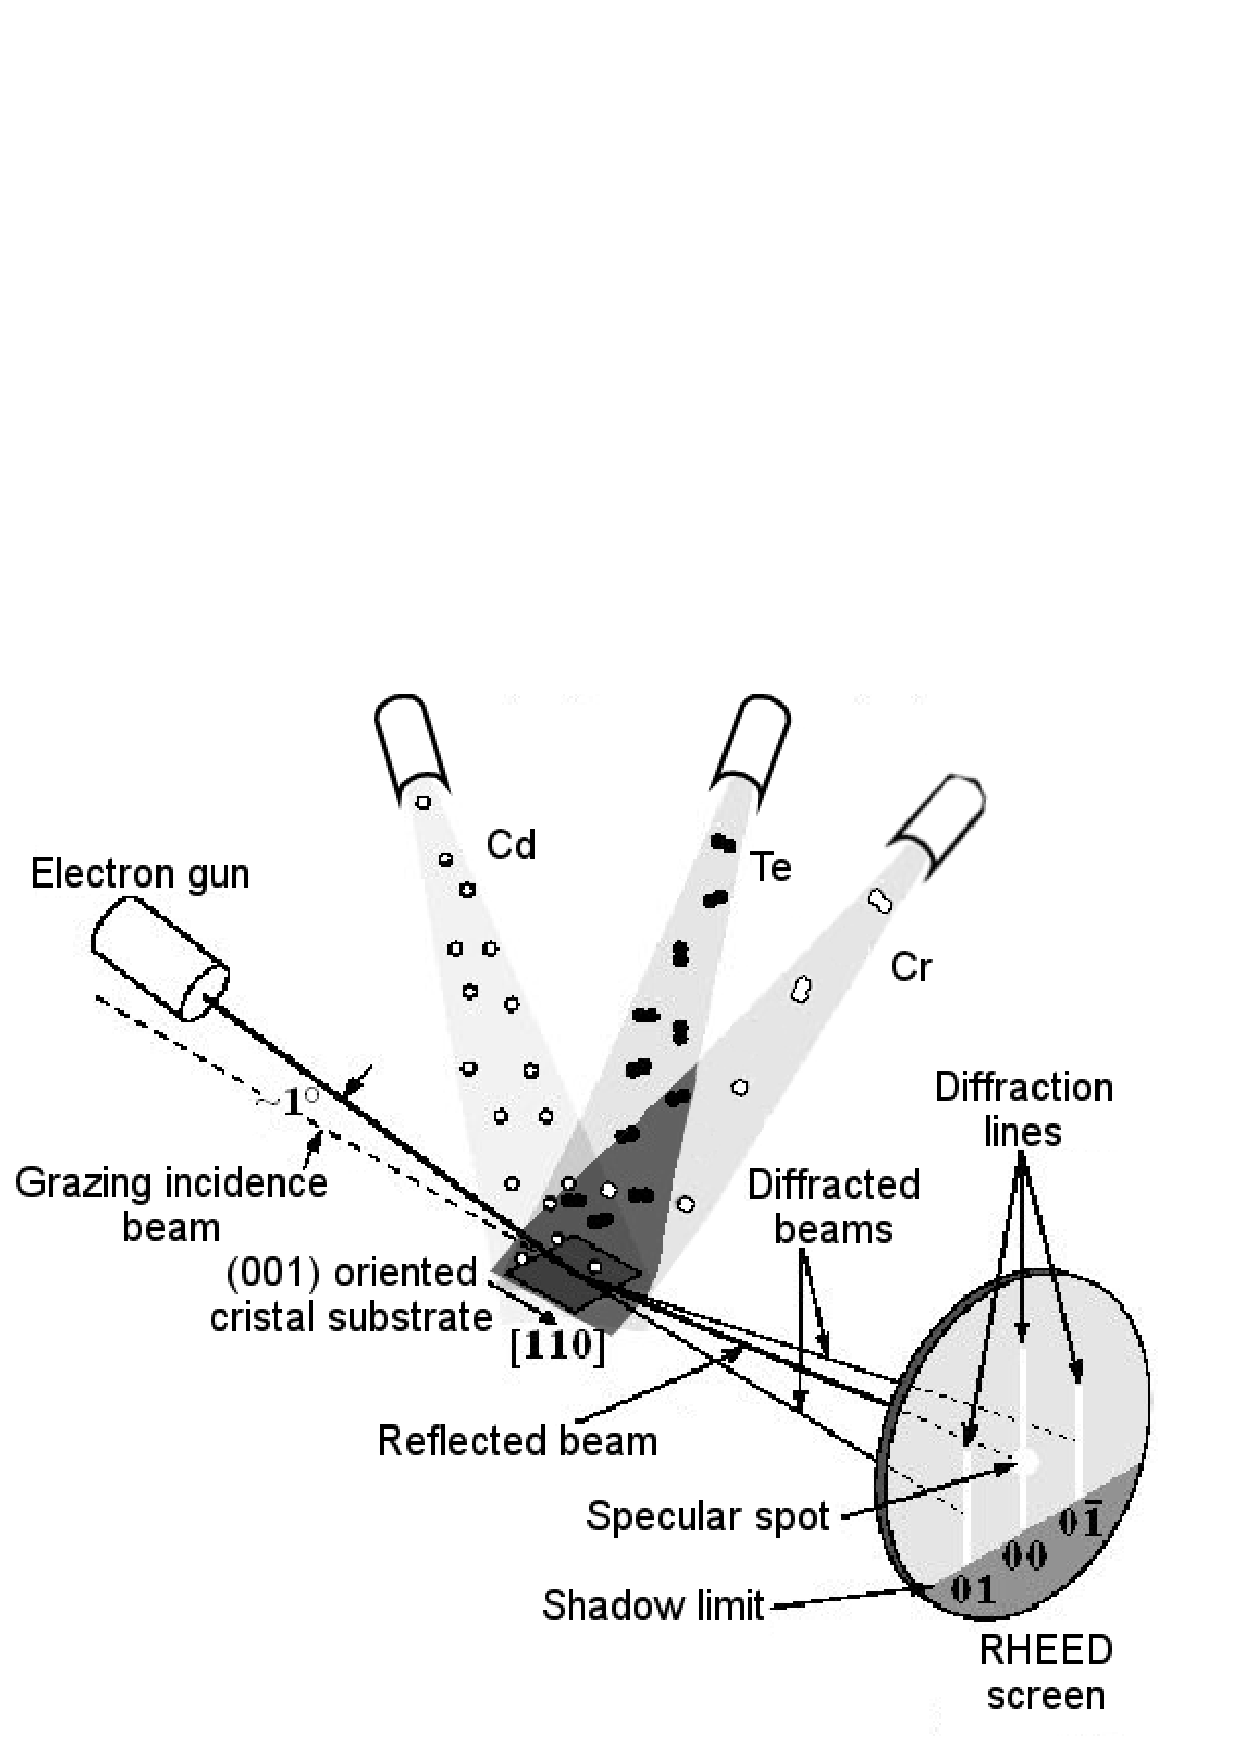
\includegraphics[width=10cm]{02-GrowthQDs/Pictures/MBE.png}
	\end{center}
	\caption{Scheme of a MBE chamber and the position of the cells in regard of the substrate.}
	\label{MBEScheme}
	\end{figure}
	
	Since MBE is a slow growth process, it ask for ultra-vacuum condition, in the order of $10^{-8}$ Pa, to avoid any contamination of the sample. Each raw material is contained in a Knudsen cell, which consist of a crucibles of high-melting-point material with a low contaminating power (typically Pyrolytic Boron Nitride) wrapped in tungsten filament which will act as heater. A small shutter close the container, and is controlled by computer along each recipe sequences.
	
	This necessity of Ultra High Vacuum kept the MBE to be developed before the end of the 1960s \cite{FirstMBE}, although the the idea was formalized at the end of the 19th century. The good control on the growth this method offer make it really useful for the development of nanostructure and nanoscience. The deposition layer by layer give the possibility to grow really thin structure, and the transition between two materials can be really abrupt, on a few monolayer (ML). Growing nano-structure is still the main use of MBE. However, this method is mainly on research purpose, its slow growth speed and hard to fulfil growth conditions being an obstacle for the industrialization of the process.
	
	Another mode of MBE were used during the growth of the samples: Atomic Layer Epitaxy (ALE) or Migration-Enhanced Epitaxy (MEE). In this mode, the opening and closing of the cells are controlled during the growth in order to deposit one element at a time, with some time between each opening for the surface to relax. For CdTe, which was used to grow our QDs layer, a substrate temperature between 260$^{\circ}$C and 290$^{\circ}$C guaranty a growth of only 0.5 ML for each cycle, which is a complete sequence of opening and closing of the cells \cite{HMarALE}. This allow a small uncertainty on the substrate temperature while keeping a really good control on the growth of the sample.
	\newline
	
	In order to monitor each step of the growth, RHEED patterns of the sample surface were taken at different key moments. This technique require a high vacuum, a given since MBE ask for ultra-high vacuum condition, and the use of an electron gun able to produce high energy electron. The beam of the gun is sent at low angle, between 1$^{\circ}$ and 3$^{\circ}$, to the surface sample. This way, the electron will only probe the surface of the sample, entering the material only on a 3 or 4 ML. Therefore the detected pattern directly gives information on the flatness and the crystallinity of the surface. The detector, a CCD camera,  is set in order to collect only elastically scattered electrons.
	
	Incident electron have a wave vector $\mathbf{k_i} = 2 \pi / \lambda_e$, with $\lambda_e$ is the electron wavelength, typically 6 or 7 pm for an electron gun energy between 30 and 40 kV. Since only scattered diffraction is considered, the diffracted wave vector $\mathbf{k_f}$ as the same norm as the incident one $\mathbf{k_i}$. So the Ewald's Sphere has a radius equal to the norm of $\mathbf{k_i}$. In the reciprocal space, the plane of diffraction are infinite line. So, in the case of a perfect crystal, with a a perfect detector, the intersection with Ewald's sphere should be points. However, since the crystal can have some defect and neither the gun or the detector are perfect, the diffracted pattern present line, such as visible on Fig.\ref{RHEEDStep}(b).
	
	Once dots are grown, though, the surface become rough at the scale of the length of coherence of the beam. Therefore, the reciprocal space of the crystal is not line anymore. The electron can interact with several more layer while passing through the dots. This can be seen on the diffraction pattern, where lines become points, such as shown on Fig.\ref{RHEEDStep}(e).
	
	Another use of the RHEED diffraction is the monitoring of the number of layer grown through ALE. Focusing on the lowest angle reflected spot, called the specular spot, one can see small variation in the reflected intensity during the growth, showing oscillation through, such as presented on Fig.\ref{RHEEDOsc}. This intensity is minimal when there is half a ML grown, and maximal when the ML is fully grown. This is due to the variation of reflectivity of the surface: maximal for a flat surface, minimal for a rough one. Therefore, a period of these oscillation is exactly the growth of a single monolayer \cite{FirstRHEED,WoodRHEED}. We can also see the relaxation of a layer, if the variation of intensity disappear at a point.
	
	\begin{figure}[h!]
	\begin{center}
		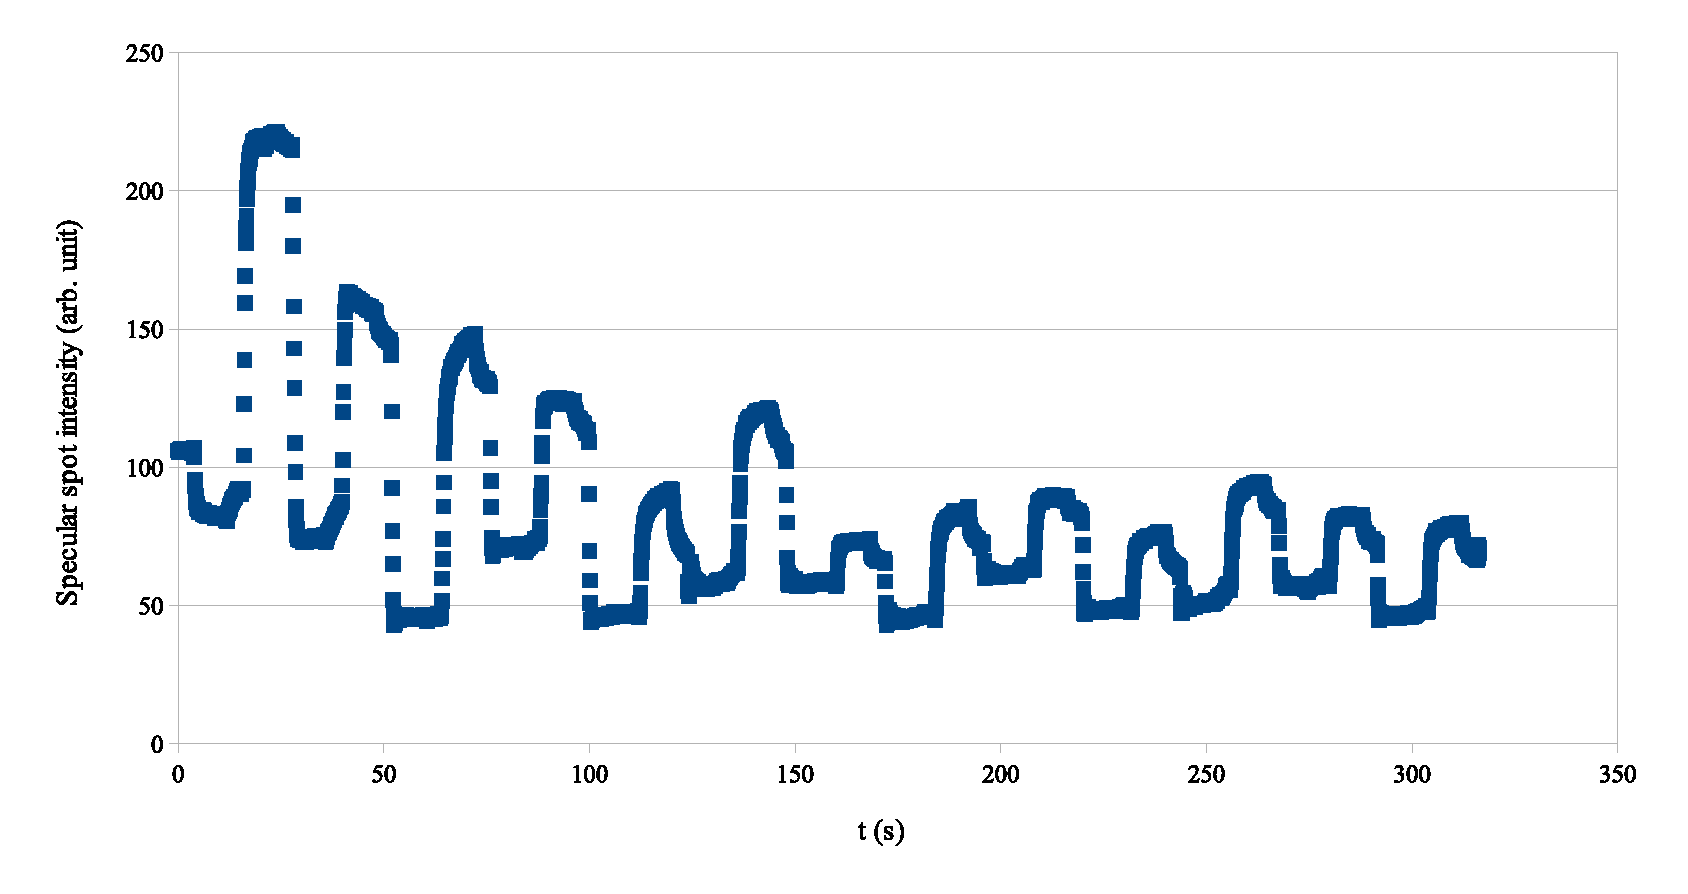
\includegraphics[width=14cm]{02-GrowthQDs/Pictures/SFDRheed.eps}
	\end{center}
	\caption{RHEED oscillation for the ALE of strained dots.}
	\label{RHEEDOsc}
	\end{figure}
	
	We studied to type of quantum dots: self assembled QDs, which have remaining strain on it, and strain free QDs. The strained dots are formed by the relaxation of a CdTe layer on ZnTe. Strain free dots are formed by thickness variation of a CdTe quantum well between CdMgTe barriers.
	
	%We are working with two sample holder, named "marked" and "unmarked", with slightly different temperature offset. The thermometer to measure the substrate temperature is placed at a few centimetre from the substrate holder, inducing another offset in the measured temperature.
	
	\section{Tsukuba machine specificity\label{Machine}}
	
	\begin{figure}[h!]
	\begin{center}
		\includegraphics[width=14cm]{02-GrowthQDs/Pictures/MBEFull.eps}
	\end{center}
	\caption{MBE machine in which the growth took place. There is 8 cells available: Aluminium, Cadmium, Chromium, Iron, Magnesium, Manganese, Tellurium and Zinc.}
	\label{MBE}
	\end{figure}
		
		Sample holder in Tsukuba were flat plates of molybdenum, in which two screw holes were pierced. The two holes were used to fix two metallic rods which maintain the sample on the holder. This way, the sample didn't move or fall during the entry in the chamber or the growth. Two sample holders were available in Tsukuba, marked and unmarked, with a temperature offset difference of about 15$^{\circ}$C.
		
		The load lock chamber can hold to samples at the same time. Beginning at this stage, the sample were put upside down, in order for the sample to face the cells when entering the main chamber. Once the two samples holder were placed the load-lock chamber, it is pump and nitrogen gas is injected in.
		
		To put a sample holder in the main chamber, it was fixed to a transfer cane via a screw hole on his back. As shown on Fig.\ref{MBE}, the cell were placed on the lower part of the MBE machine, so the sample holder as to be put upside down in the main chamber in order to face them. Once in the chamber, the sample temperature was measured through a thermocouple at a few centimetre from the sample holder. This distance induced an offset on the measured temperature. This was important in the ALE to be in the temperature interval where 0.5 ML are grown each cycle. The temperature was therefore calibrated in order to grow the right number of monolayer for each growth (see part \ref{SKGrowth} and \ref{SFDGrowth}). The system being really stable in time, we kept this calibration for all the growth.
		
		The flux of each cells was calculated using Beam Equivalent Pressure (BEP) in the main chamber. The pressure in the main chamber was measured with a nude ionization gauge, both before and after having opened a single cell. Subtracting these two numbers gave us the BEP of the cell. The pressure in the main chamber was typically between $1.0 \times 10^{-9}$ Torr and $1.0 \times 10^{-8}$ Torr.
Since the growth speed depend on the flux of the cell, we used this method to control it: we first calibrate the growth speed in function of the pressure in the chamber, and then used these equivalence to control the growth process.
		
	\section{Strained dots: CdTe/ZnTE\label{SK}}
	
	\subsection{Substrate preparation}
	
		The sample was grown on ZnTe(100) substrates. We prepared the substrate by deosoxidizing them through an etching process. It was done in four steps. All of them, except the etching in Bromure-ethanol, occur in an ultrasonic cleaning device vibrating the sample at 43kHz and last 3 minutes. We began with  cleaning in acetone, followed by one in ethanol. The third step was the actual etching: the substrate was put in a solution of Bromure-ethanol, with 3\% of Bromure, during 1 minute. We finally rinsed it in methanol. Once rinsed, we keep the sample in ethanol until fixing them to the sample holder. The growth usually occur the day after the cleaning.
	
	\subsection{Strained dots growth\label{SKGrowth}}
	
	Before beginning the actual growth, after we entered the sample in the main chamber, we had to heat the cells and the sample, and to do the flux calibration for each cell. The targeted flux and heating speed are presented in Tab.\ref{FluxTempSK} for each cell used during the growth of strained QDs. 
	
	\begin{table}[h!]
	\begin{center}		
		\begin{tabular}{| c | c |}
			\hline
			Elements & Targeted BEP (Torr) \\ \hline
			Cd & $4.5\times10^{-7}$ \\
			Cr & N/A \\
			Te & $4.5\times10^{-7}$ \\
			Zn & $6.8\times10^{-7}$ \\
			\hline
		\end{tabular}
		\caption{Aimed flux for each cell during the growth of the strained QDs.}
		\label{FluxTempSK}
	\end{center}
	\end{table}
	
	It was shown that the to have a good quality of material, it was better to grow the ZnTe in excess of Zn \cite{TeEffect}. Otherwise, vacancies appear in the bulk, optically visible, and the surface is more rough. Moreover, the adsorption power of the Zn is smaller than the Te. For these reason, we choose to grow the ZnTe barriers in excess of Zn.
	
	When the sample is exposed to either Cd or Te flux during ALE, only one atomic layer will be deposited under each flux: we call this \emph{auto-regulated} growth. So, we chose the same flux for both of the compound \cite{HMarALE}. 
	
	Beginning the growth, the substrate temperature was initially raised to $320^{\circ}$C. The Zn cell shutter was open starting at $250^{\circ}$C, in order to flatten the surface for the growth. While it took several minutes to raise the substrate temperature, only one Zn layer can be deposited at a time. When the substrate temperature reach $320^{\circ}$C, the Te shutter was also open, in order to grow a ZnTe layer of about $420$ nm, at about $0.4$ ML.s$^{-1}$. This thick ZnTe layer guaranteed us to the best possible surface for the growth of the QD layer \cite{ChangZnTe}. Once done, we set up the RHEED, growing a few more ZnTe level while searching the specular spot. The substrate temperature was then lowered to $195^{\circ}$C (marked sample holder) or $180^{\circ}$C (unmarked sample holder), the Zn cell being open until the temperature reach $250^{\circ}$C. Then, the ALE began.
	
	\begin{figure}[h!]
	\begin{center}
		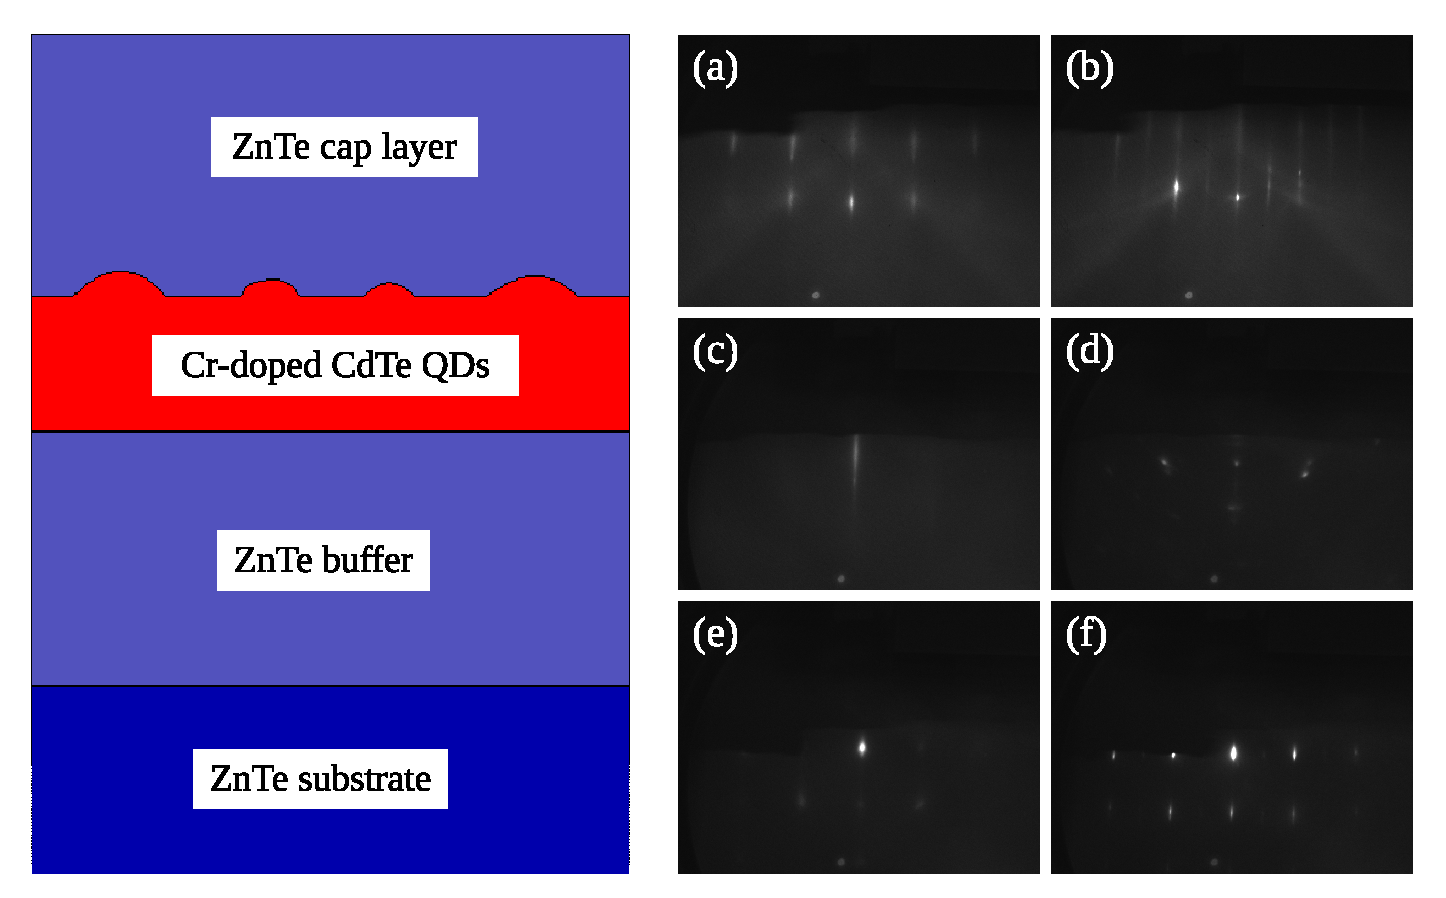
\includegraphics[width=14cm]{02-GrowthQDs/Pictures/RHEEDStep.eps}
	\end{center}
	\caption{Left: Layer structure of the strain Cr-doped CdTe QDs samples.
		Right: RHEED pattern taken at different key moment of the growth: (a) before the growth of the ZnTe buffer, (b) after the growth of the ZnTe buffer, (c) after the (Cd,Cr)Te ALE, (d) after the Te deposition, (e) during the Te evaporation (the picture was taken at T$_{substrate} = 177^{\circ}$C) and (f) after the growth of the ZnTe cap.}
	\label{RHEEDStep}
	\end{figure}
	
	One of the main difficulty of this work was to calibrate the Cr flux in order to trap only a single Cr atom in most of the QDs of the sample. To achieve so, the Cr density must be of the same order as the QDs density at the surface of the sample. This means a really small flux, with a BEP of some $10^{-10}$ Torr, which is about one order lower than the main chamber pressure and therefore not measurable with our technique. The optimisation was done starting with the know how acquired in Grenoble on the Mn and trying to optimise it for the Tsukuba machine, through a feedback loop with the micro-PL characterization in Grenoble.

	
	This really small flux was achieve by heating the Cr cell around 1000K, low compared to its sublimation temperature, and opening the cell only once during the ALE, for only 5s. In order to have big enough QDs, emitting at right wavelengths, we needed 6.5 ML of CdTe. Going above this number will create dislocation and defects in the layer, preventing it to relax correctly to form the QDs. To do so, we had to do 13 cycles of Cd and Te cells opening, since each cycle grew half a layer. However, these 6.5 ML of CdTe don't relax naturally: we had to deposit Te above and evaporate before seeing the formation of the dots \cite{TinjodMBE}. The Cr cells was opened during the 7th cycle, halfway through the growth of the QD layer, in order to allow the Cr atoms to diffuse without going out the QD layers. The whole ALE recipe to grow the QDs layer is given in the Fig.\ref{RecipeSK}.
	
	\begin{figure}[h!]
	\begin{center}
		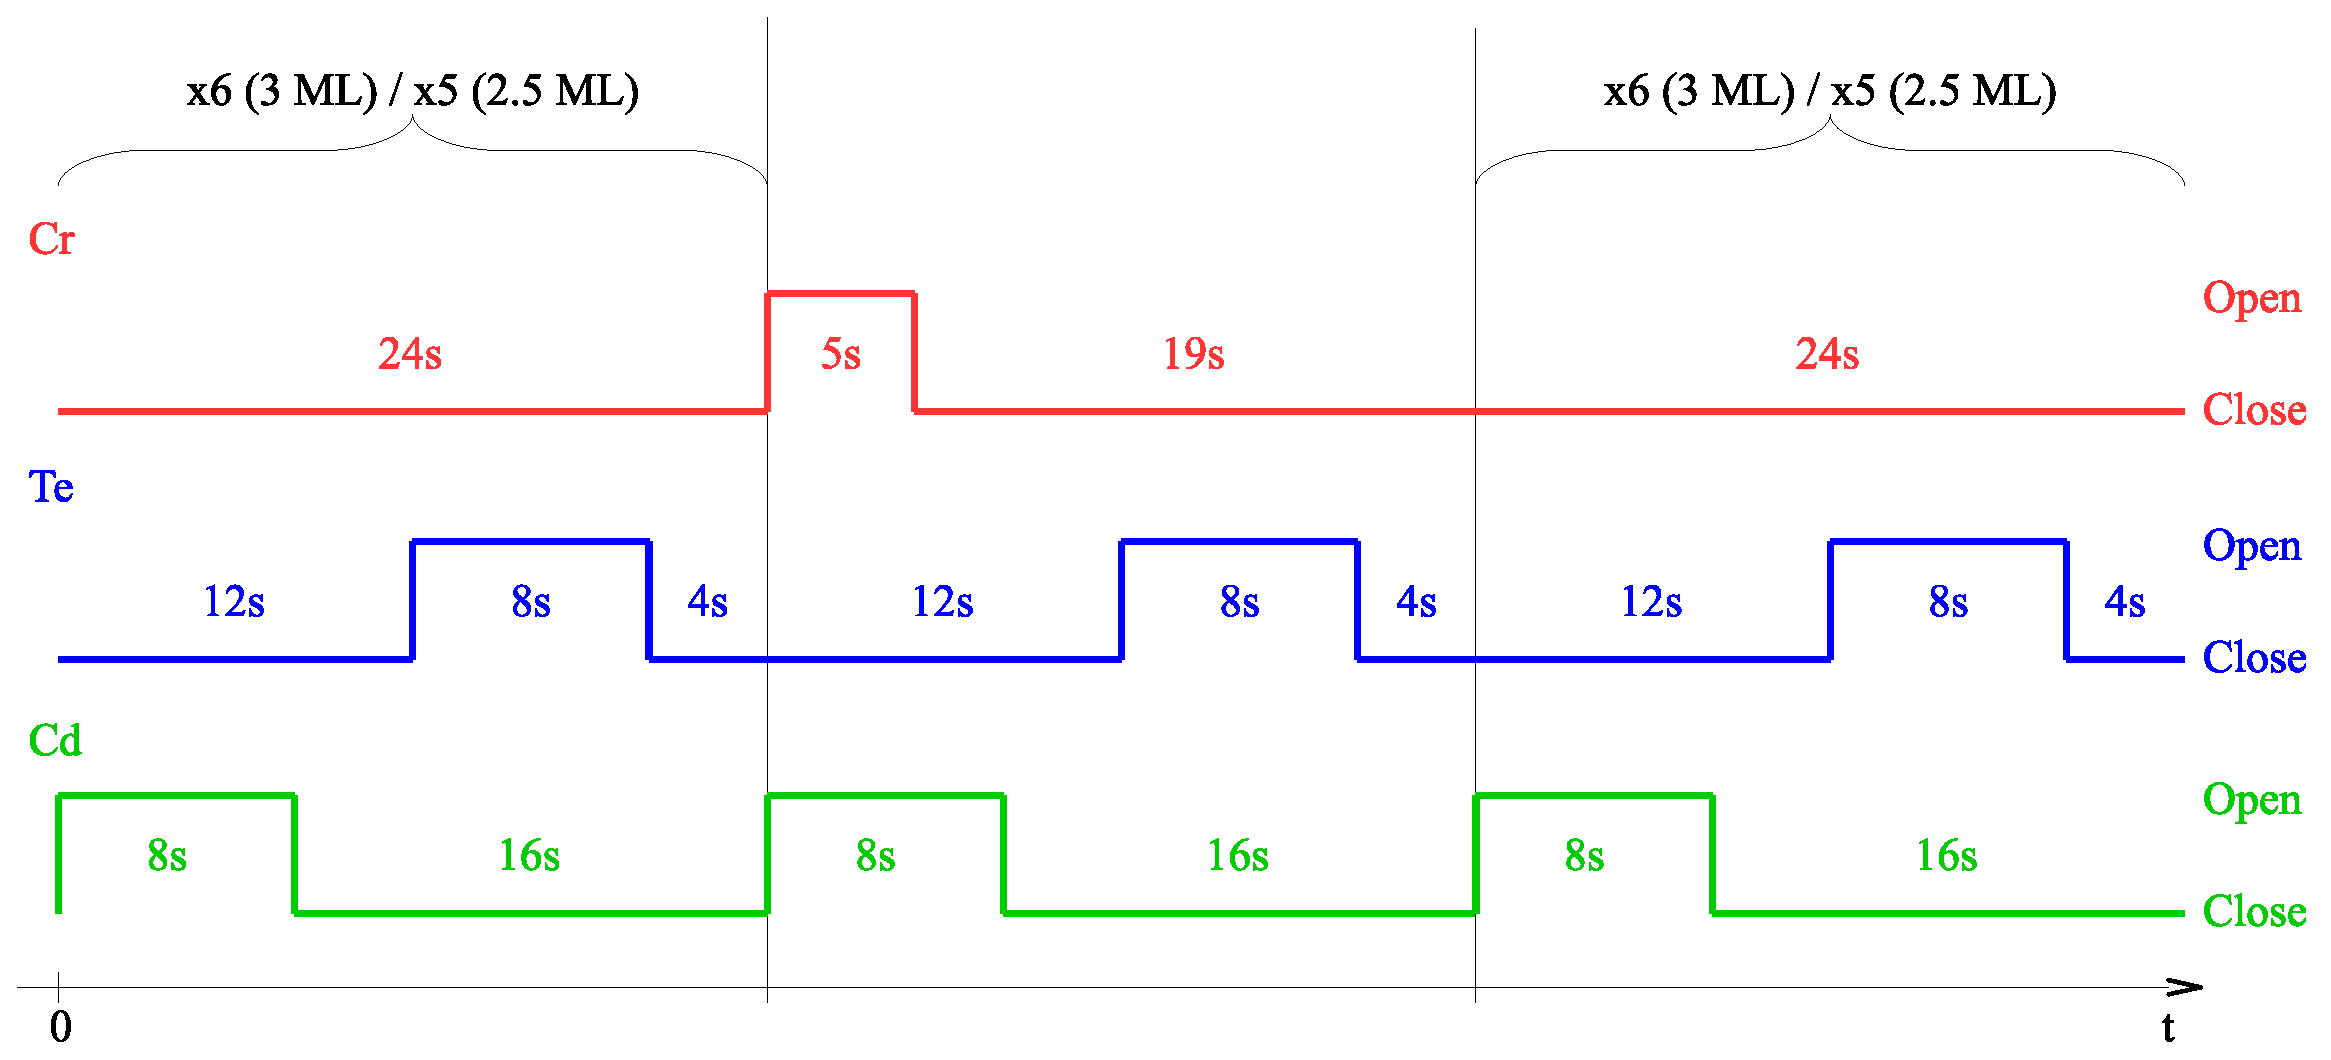
\includegraphics[width=14cm]{02-GrowthQDs/Pictures/RecipeSK.eps}
	\end{center}
	\caption{Opening and closing cycles of each cell for the ALE of strained (Cd,Cr)Te samples.}
	\label{RecipeSK}
	\end{figure}

	Once the ALE was finished, we lowered the substrate temperature to $90^{\circ}$C to deposit the Te layer which formed the dots. It was deposited during 5 minutes. We then heated up the substrate again until $200^{\circ}$C, were we stayed for 20s in order to evaporate all the deposited Te \cite{WojnarMBE}. If the dots were formed, we saw a spotty pattern like the one presented on Fig.\ref{RHEEDStep} (f). The Zn and Te cells were then opened, while the substrate temperature was raised to $240^{\circ}$C in order to grow a protective layer about $350$ nm thick above the QDs.
	
	\section{Strain-free dots: CdTe/CdMgTe\label{SFD}}
		\subsection{Substrate preparation}
		
		The barrier for strain free samples are made of CdTe. The chosen substrate for the growth was GaAs, on which we grew a layer of about 3 $\mu$m of CdTe. Growing such a thick layer guaranty that the remaining strain are in the order of $0.1\%$ \cite{StrainRelaxCdTeGaAs111,StrainRelaxCdTeGaAs100}. Moreover, a small ZnTe layer was grown between GaAs and CdTe, which accelerated the relaxation of the strains \cite{StrainRelaxZnTeGaAs001}.
		
		For this sample, only a simple cleaning occur outside of the MBE machine. We did it in four steps, each of them lasting for 5 minutes in an ultrasonic cleaning device. We began with a cleaning acetone, at 43 kHz, followed by one in ethanol at the same frequency. We then put the substrate in water and clean it at 43 kHz. Finally, we changed the water and did the last step in water at 23 kHz, in order to clean the substrate from smaller dust particle.
		
		Since the surface of the GaAs is oxidized, no RHEED pattern was visible, as shown on Fig \ref{Hybrid}(a). The desoxidation was done in the MBE main chamber, in vacuum condition, using hydrogen radical (H$^*$). In order to form the radical gas, a hydrogen gas was ionized in a chamber by a RF power source of 300 W and with a frequency of 13.6 MHz. This gas composition is optically checked by probing the emission of the Balmer serie: for a pure hydrogen gas, peaks at 656 nm and 486 nm appear clearly. During the formation of this gas, the substrate temperature is raised to $400^{\circ}$C. Once the hydrogen chamber is full of H$^*$ gas, we initiate the rotation of the sample. Since the chamber was situated just under the main and linked to her, we just had to open the shutter between the two to send the radical gas onto the substrate. We exposed the substrate to this gas for 15 minutes, under a pressure of about $6\times10^{-7}$ Torr. We then checked the sample surface with RHEED, which should present a streak pattern with some dots as presented in Fig \ref{Hybrid}(b). 
		
		Once the cleaning of the sample was finished, we closed the H$^*$ gas chamber shutter, waited for the ultra-high vacuum to re-established in the main chamber and began the growth of the CdTe layer. We grew it in two times: one hour of growth just after the cleaning (described here) and about four hours just before the actual growth of  the quantum dots structure.
		
	\begin{figure}[h!]
	\begin{center}
		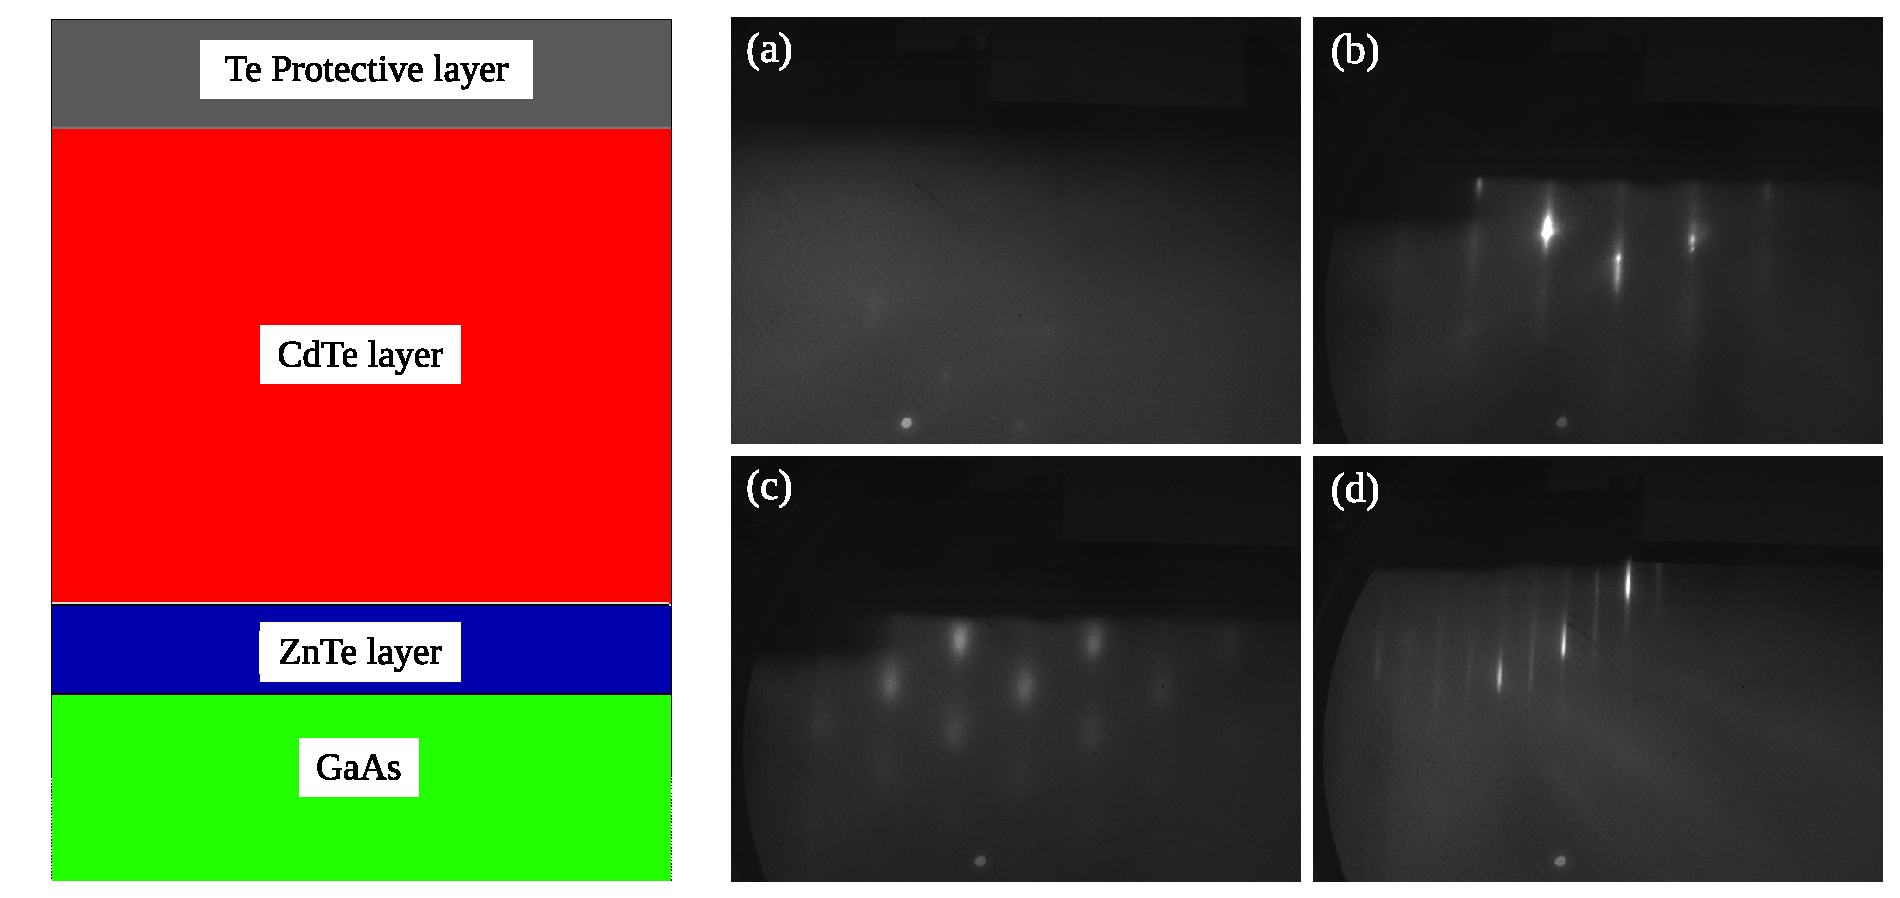
\includegraphics[width=14cm]{02-GrowthQDs/Pictures/HybridSubstrate.eps}
	\end{center}
	\caption{Left: Layer structure of the hybrid substrate with its protective Te cap.
		Right: RHEED pattern taken at different key moment of the growth: (a) before H$^*$ cleaning of GaAs, (b) after H$^*$ cleaning of GaAs, (c) after the growth of the ZnTe layer, (d) after the growth of the CdTe layer.}
	\label{Hybrid}
	\end{figure}
		
		This first part of the growth took place on a rotating sample. It only take about 15 ML of ZnTe on GaAs for the II-VI compound go back to its original lattice parameter \cite{StrainRelaxZnTeGaAs001}. Moreover, CdTe over ZnTe has a critical thickness of 5 ML \cite{CritThickCdTeZnTe}. So, to accelerate the relaxation of strain, we decided to grow a thing layer of ZnTe above the GaAs, before growing the CdTe thick layer. We lowered the substrate temperature to $320^{\circ}$C and opened the Zn cells for 30s with a BEP of $7.05\times10^{-7}$ Torr in order to flatten the surface. We then opened the Te cells, with a BEP of $5.21\times10^{-7}$ Torr, along with the Zn cell during 50s to grow the ZnTe layer in excess of Zn, making a layer about 7.2 nm thick.
		
		We then went to the growth of the first CdTe layer. We lowered again the substrate temperature to $250^{\circ}$C, under Zn flux. Once stabilized at the temperature, we closed Zn cells and open the Cd and Te cells for 1h. The Te cell had the same flux as previously, while the Cd cells had a flux of $4.72\times10^{-7}$ Torr. This layer was 633 nm thick, grown at 0.54 ML.s$^{-1}$. In order to protect the surface, we deposit an amorphous protective layer of Te above it, while decreasing the substrate temperature.
		
		\subsection{Unstrained dots growth\label{SFDGrowth}}
		
	As said in the introduction, the strain free dots are formed by thickness variation of a CdTe QW surrounded by CdMgTe barrier. In order to have to good confinement while keeping a close enough lattice constant, we chose to use Cd$_{0.7}$Mg$_{0.3}$Te. Therefore, the first step of the growth was to chose the flux for the growth. We went through a process of trial and error, growing several samples and testing their composition with Electron Probe Mico-Analysis and X-Ray diffraction, as well as the thickness grown with a step gauge, in order to estimate the growth speed. Since we wanted to grow Cd$_{0.7}$Mg$_{0.3}$Te, we began the test with a ration Te:Cd of 1:0.7 and a ratio Te:Mg of 1:0.3. After five round of adjustment, we achieve the growth of Cd$_{0.7}$Mg$_{0.3}$Te, settling with the targeted flux presented in Tab.\ref{FluxTempSFD}.
	For the settled Mg flux, the step gauge indicated a grown thickness of $520 \pm 5$ nm. Since we grew the test layer during 1h, we found a growing speed of about 0.15 nm.s$^{-1}$.
	\begin{table}[h!]
	\begin{center}		
		\begin{tabular}{| c | c |}
			\hline
			Elements & Targeted BEP (Torr) \\ \hline
			Cd & $4.5\times10^{-7}$ \\
			Cr & N/A \\
			Mg & $1.6\times10^{-8}$ \\
			Te & $5.26\times10^{-7}$ \\
			\hline
		\end{tabular}
		\caption{Aimed flux for each cell during the growth of the strained samples.}
		\label{FluxTempSFD}
	\end{center}
	\end{table}
	
	We began to heat the substrate temperature to 180$^{\circ}$, in order to remove the protective amorphous Te layer. We waited a few second at this temperature to remove all the deposited Te, and then resumed the heating to go to $250^{\circ}$C. Starting at $200^{\circ}$C, we opened the Te cells in order to stabilize the surface. When the substrate temperature was stabilized at $250^{\circ}$C, we opened the Cd cells and grew a 2.35 $\mu$m layer of CdTe, in order to reach the thickness of the relaxation of strains for CdTe/GaAs \cite{StrainRelaxCdTeGaAs111,StrainRelaxCdTeGaAs100}.
	
	In order to be sure that there will be no relaxation in the quantum, we choose to stick to the maximum cumulated thickness of the CdTe on a CdZnTe lattice, which has been shown to be lower than the one of CdTe on a CdMgTe lattice. This correspond to a maximum cumulated thickness of 130 nm \cite{CritThickCdTeCdZnTe}. We chose to grow 40 nm below the QW, and 90 nm above it, in order to have a thicker protective layer.

	Once the 40 nm barrier layer was grown, we lowered the substrate temperature under Te flux. Growing the QW layer in a Te environment smooth the surface layer of the sample and help having a flat surface to grow the well. Once the substrate temperature reach respectively $180^{\circ}$C (unmarked) or $195^{\circ}$C (marked), we began the ALE of the QW.
[insert explication on the Cr SFD ALE here]
The recipe is described in Fig.\ref{RecipeSFD}.
	\begin{figure}[h!]
	\begin{center}
		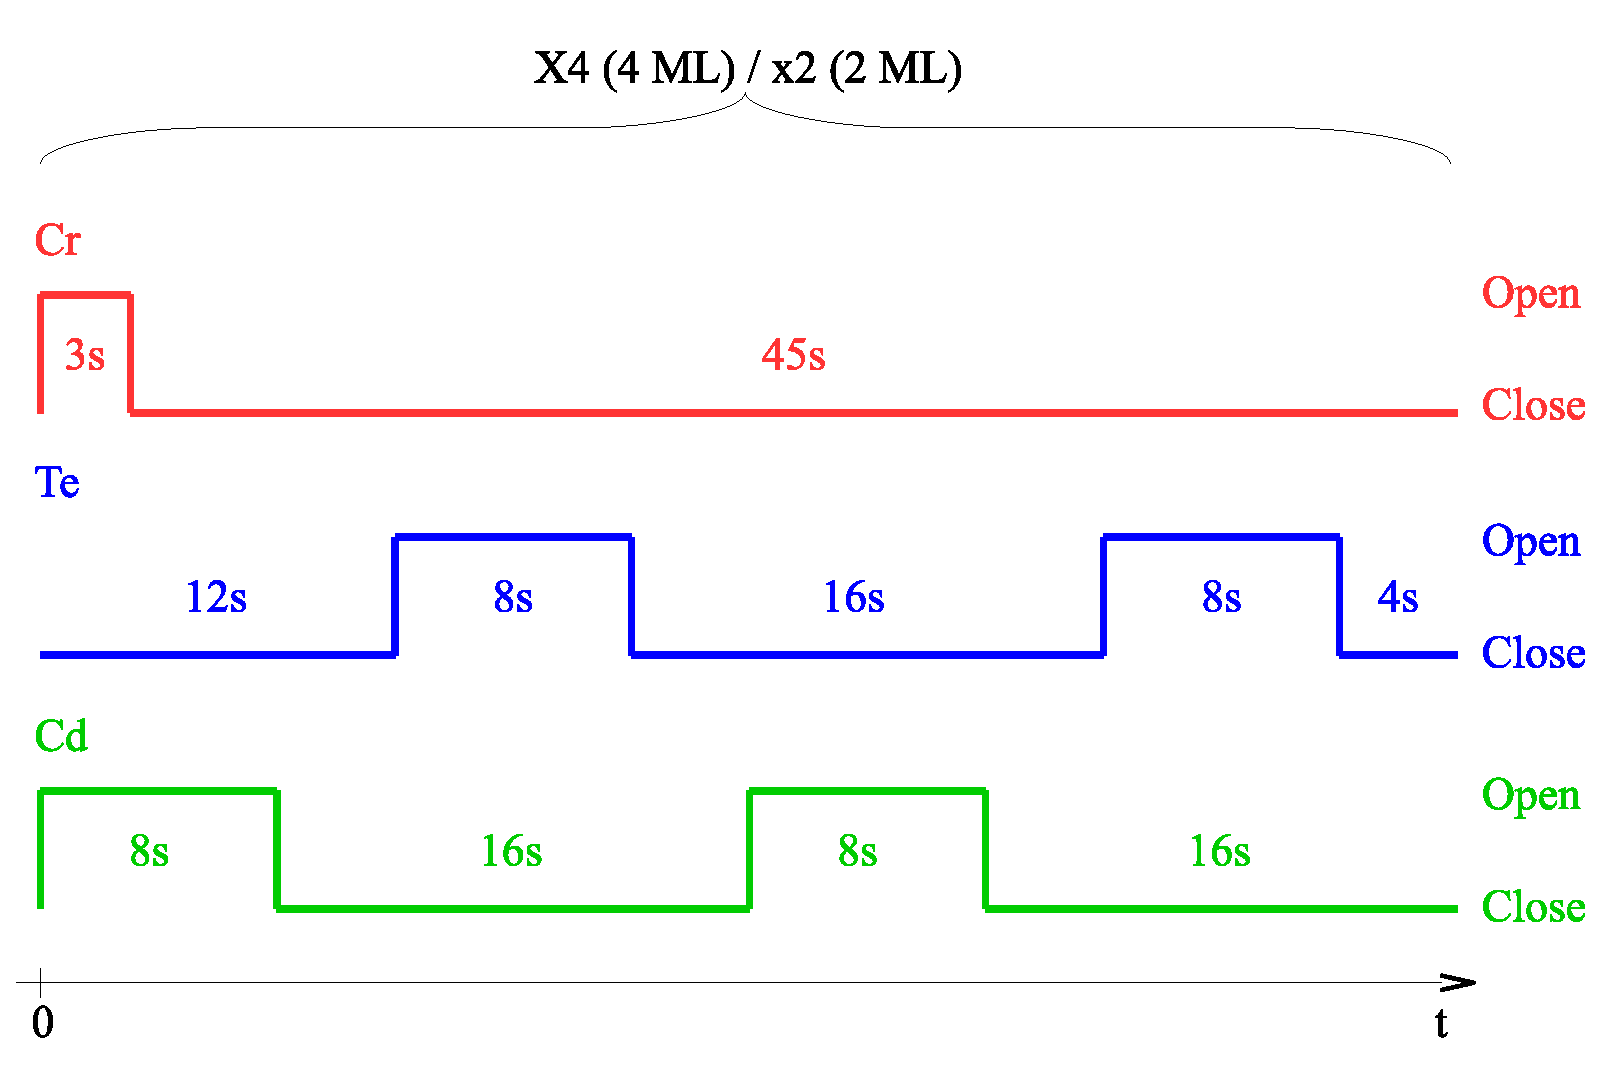
\includegraphics[width=14cm]{02-GrowthQDs/Pictures/RecipeSFD.eps}
	\end{center}
	\caption{Opening and closing cycles of each cell for the ALE of strain free (Cd,Cr)Te samples. (not accurate - 12/2015)}
	\label{RecipeSFD}
	\end{figure}
We then raised the substrate temperature up to $250^{\circ}$C, under a Te flux, in order to proceed to the growth of the upper barrier, acting also as a protective layer. The opening time was there calculated to grow 90 nm of Cd$_{0.7}$Mg$_{0.3}$Te.






\chapter{Coherent dynamics of Mn-doped positively charged quantum dots}

	\section{Mn in a II-VI positively charged quantum dot}

	Cf Optical control of the spin of a magnetic atom in a semiconductor QD, L. Besombes et. al., Sept 2014
	
		\subsection{Quantum dot charged state selection\label{ChargeSelec}}
		
		Lorem ipsum dolor sit amet, consectetur adipiscing elit. Curabitur tortor quam, imperdiet quis facilisis sed, fringilla a quam. Cras ante odio, hendrerit ac ante nec, cursus imperdiet urna. Mauris convallis ultricies purus, nec condimentum erat bibendum vel. Aliquam erat volutpat. Pellentesque condimentum, eros a consequat accumsan, turpis sem euismod nisi, sed fringilla quam turpis sit amet erat. Mauris dictum odio sed nisi dapibus, et molestie mauris rutrum. Praesent convallis dolor in nibh blandit bibendum. Quisque sit amet arcu consectetur lorem luctus venenatis nec quis dui. Aliquam erat volutpat. Aenean auctor elit nec tristique dignissim. Nulla massa mi, efficitur semper ex id, pretium eleifend massa. Vivamus sit amet orci scelerisque, gravida est ut, vulputate odio.
		
	\begin{figure}[h!]
	\begin{center}
		\includegraphics[width=10cm]{FillingPicture.png}
	\end{center}
	\caption{Sample with Schottky gate and micro-lens}
	\label{Schottky}
	\end{figure}

	Curabitur eget ipsum egestas dui viverra suscipit. Cras aliquet lacus vitae erat finibus semper. Nulla pharetra eget urna vitae sodales. Nunc faucibus velit lacus, nec ornare eros aliquet quis. Donec a orci nec sem pulvinar ultricies sit amet ut arcu. Nullam id vehicula enim, at tincidunt velit. Duis vestibulum lorem a molestie fringilla. Nullam tincidunt semper placerat. Donec nibh sem, ornare eget cursus ac, luctus sit amet eros. Phasellus eget interdum nisi. Donec mollis risus id lectus fringilla, et commodo risus iaculis. Donec at lacus sed nibh posuere posuere sit amet eget sapien. In dignissim, enim sit amet convallis fermentum, lacus nulla gravida tortor, non facilisis ex nisl sit amet augue. Maecenas eu enim condimentum, consectetur ligula vel, tincidunt nisl. Nam laoreet dictum volutpat. Donec at erat venenatis, ultrices lorem ac, vestibulum neque.

	\begin{figure}[h!]
	\begin{center}
		\includegraphics[width=10cm]{FillingPicture.png}
	\end{center}
	\caption{Example of charge variation and selection of the charged state}
	\label{StateSelection}
	\end{figure}
		
		\subsection{Energy structure}
		
		Cf XplusMnRes.pptx to detail the e-Mn levels
		
	\begin{figure}[h!]
	\begin{center}
		\includegraphics[width=10cm]{FillingPicture.png}
	\end{center}
	\caption{X+-Mn spectra and linear polarization}
	\label{Spectra&LinPolar}
	\end{figure}
		
		Lorem ipsum dolor sit amet, consectetur adipiscing elit. Curabitur tortor quam, imperdiet quis facilisis sed, fringilla a quam. Cras ante odio, hendrerit ac ante nec, cursus imperdiet urna. Mauris convallis ultricies purus, nec condimentum erat bibendum vel. Aliquam erat volutpat. Pellentesque condimentum, eros a consequat accumsan, turpis sem euismod nisi, sed fringilla quam turpis sit amet erat. Mauris dictum odio sed nisi dapibus, et molestie mauris rutrum. Praesent convallis dolor in nibh blandit bibendum. Quisque sit amet arcu consectetur lorem luctus venenatis nec quis dui. Aliquam erat volutpat. Aenean auctor elit nec tristique dignissim. Nulla massa mi, efficitur semper ex id, pretium eleifend massa. Vivamus sit amet orci scelerisque, gravida est ut, vulputate odio.
		
	\begin{figure}[h!]
	\begin{center}
		\includegraphics[width=10cm]{FillingPicture.png}
	\end{center}
	\caption{Mn in charged QD simple energy structure}
	\label{SimpleEnerStruct}
	\end{figure}

	Curabitur eget ipsum egestas dui viverra suscipit. Cras aliquet lacus vitae erat finibus semper. Nulla pharetra eget urna vitae sodales. Nunc faucibus velit lacus, nec ornare eros aliquet quis. Donec a orci nec sem pulvinar ultricies sit amet ut arcu. Nullam id vehicula enim, at tincidunt velit. Duis vestibulum lorem a molestie fringilla. Nullam tincidunt semper placerat. Donec nibh sem, ornare eget cursus ac, luctus sit amet eros. Phasellus eget interdum nisi. Donec mollis risus id lectus fringilla, et commodo risus iaculis. Donec at lacus sed nibh posuere posuere sit amet eget sapien. In dignissim, enim sit amet convallis fermentum, lacus nulla gravida tortor, non facilisis ex nisl sit amet augue. Maecenas eu enim condimentum, consectetur ligula vel, tincidunt nisl. Nam laoreet dictum volutpat. Donec at erat venenatis, ultrices lorem ac, vestibulum neque.
	
	\begin{figure}[h!]
	\begin{center}
		\includegraphics[width=10cm]{FillingPicture.png}
	\end{center}
	\caption{Energy structure of h-Mn/X+-Mn with valence band mixing, perturbative two holes, with the linear polarization as an example (experiment + model)}
	\label{CompleteEnerStruct}
	\end{figure}
	
	Curabitur eget ipsum egestas dui viverra suscipit. Cras aliquet lacus vitae erat finibus semper. Nulla pharetra eget urna vitae sodales. Nunc faucibus velit lacus, nec ornare eros aliquet quis. Donec a orci nec sem pulvinar ultricies sit amet ut arcu. Nullam id vehicula enim, at tincidunt velit. Duis vestibulum lorem a molestie fringilla. Nullam tincidunt semper placerat. Donec nibh sem, ornare eget cursus ac, luctus sit amet eros. Phasellus eget interdum nisi. Donec mollis risus id lectus fringilla, et commodo risus iaculis. Donec at lacus sed nibh posuere posuere sit amet eget sapien. In dignissim, enim sit amet convallis fermentum, lacus nulla gravida tortor, non facilisis ex nisl sit amet augue. Maecenas eu enim condimentum, consectetur ligula vel, tincidunt nisl. Nam laoreet dictum volutpat. Donec at erat venenatis, ultrices lorem ac, vestibulum neque.
	
	\begin{figure}[h!]
	\begin{center}
		\includegraphics[width=10cm]{FillingPicture.png}
	\end{center}
	\caption{Linear polarization modelization with variation of parameter to show influence.}
	\label{LinPolModelMn}
	\end{figure}
		
		\subsection{Optical $\lambda$-level identification}	
		
		Lorem ipsum dolor sit amet, consectetur adipiscing elit. Curabitur tortor quam, imperdiet quis facilisis sed, fringilla a quam. Cras ante odio, hendrerit ac ante nec, cursus imperdiet urna. Mauris convallis ultricies purus, nec condimentum erat bibendum vel. Aliquam erat volutpat. Pellentesque condimentum, eros a consequat accumsan, turpis sem euismod nisi, sed fringilla quam turpis sit amet erat. Mauris dictum odio sed nisi dapibus, et molestie mauris rutrum. Praesent convallis dolor in nibh blandit bibendum. Quisque sit amet arcu consectetur lorem luctus venenatis nec quis dui. Aliquam erat volutpat. Aenean auctor elit nec tristique dignissim. Nulla massa mi, efficitur semper ex id, pretium eleifend massa. Vivamus sit amet orci scelerisque, gravida est ut, vulputate odio.

	\begin{figure}[h!]
	\begin{center}
		\includegraphics[width=10cm]{FillingPicture.png}
	\end{center}
	\caption{Luminescence under laser scan (map)}
	\label{ResPLE}
	\end{figure}

	Curabitur eget ipsum egestas dui viverra suscipit. Cras aliquet lacus vitae erat finibus semper. Nulla pharetra eget urna vitae sodales. Nunc faucibus velit lacus, nec ornare eros aliquet quis. Donec a orci nec sem pulvinar ultricies sit amet ut arcu. Nullam id vehicula enim, at tincidunt velit. Duis vestibulum lorem a molestie fringilla. Nullam tincidunt semper placerat. Donec nibh sem, ornare eget cursus ac, luctus sit amet eros. Phasellus eget interdum nisi. Donec mollis risus id lectus fringilla, et commodo risus iaculis. Donec at lacus sed nibh posuere posuere sit amet eget sapien. In dignissim, enim sit amet convallis fermentum, lacus nulla gravida tortor, non facilisis ex nisl sit amet augue. Maecenas eu enim condimentum, consectetur ligula vel, tincidunt nisl. Nam laoreet dictum volutpat. Donec at erat venenatis, ultrices lorem ac, vestibulum neque.
	
	\begin{figure}[h!]
	\begin{center}
		\includegraphics[width=10cm]{FillingPicture.png}
	\end{center}
	\caption{Identification of $\lambda$-systems with each $\lambda$-system drawn}
	\label{LambdaLevem}
	\end{figure}
			
	
	\section{Spin dynamics under resonant excitation}
	
		Cf article 2016/01
	
		\subsection{Cycling and escaping the $\lambda$-level system}

		Mn in a lattice -> modification of orbital -> spin-orbit interaction. Magnetic anisotropy + anisotropy of strain. (Mn has nuclear spin 5/2 -> hyperfine interaction?)

	\begin{figure}[h!]
	\begin{center}
		\includegraphics[width=10cm]{FillingPicture.png}
	\end{center}
	\caption{Isolated $\lambda$-system with the loop (excitation, recombination, relaxation to initial state)}
	\label{LambdLoop}
	\end{figure}
		
		Lorem ipsum dolor sit amet, consectetur adipiscing elit. Curabitur tortor quam, imperdiet quis facilisis sed, fringilla a quam. Cras ante odio, hendrerit ac ante nec, cursus imperdiet urna. Mauris convallis ultricies purus, nec condimentum erat bibendum vel. Aliquam erat volutpat. Pellentesque condimentum, eros a consequat accumsan, turpis sem euismod nisi, sed fringilla quam turpis sit amet erat. Mauris dictum odio sed nisi dapibus, et molestie mauris rutrum. Praesent convallis dolor in nibh blandit bibendum. Quisque sit amet arcu consectetur lorem luctus venenatis nec quis dui. Aliquam erat volutpat. Aenean auctor elit nec tristique dignissim. Nulla massa mi, efficitur semper ex id, pretium eleifend massa. Vivamus sit amet orci scelerisque, gravida est ut, vulputate odio.

	\begin{figure}[h!]
	\begin{center}
		\includegraphics[width=10cm]{FillingPicture.png}
	\end{center}
	\caption{Pumping experiment on each $\lambda$-system}
	\label{AllPumpB0}
	\end{figure}

	Curabitur eget ipsum egestas dui viverra suscipit. Cras aliquet lacus vitae erat finibus semper. Nulla pharetra eget urna vitae sodales. Nunc faucibus velit lacus, nec ornare eros aliquet quis. Donec a orci nec sem pulvinar ultricies sit amet ut arcu. Nullam id vehicula enim, at tincidunt velit. Duis vestibulum lorem a molestie fringilla. Nullam tincidunt semper placerat. Donec nibh sem, ornare eget cursus ac, luctus sit amet eros. Phasellus eget interdum nisi. Donec mollis risus id lectus fringilla, et commodo risus iaculis. Donec at lacus sed nibh posuere posuere sit amet eget sapien. In dignissim, enim sit amet convallis fermentum, lacus nulla gravida tortor, non facilisis ex nisl sit amet augue. Maecenas eu enim condimentum, consectetur ligula vel, tincidunt nisl. Nam laoreet dictum volutpat. Donec at erat venenatis, ultrices lorem ac, vestibulum neque.
	
	\begin{figure}[h!]
	\begin{center}
		\includegraphics[width=10cm]{FillingPicture.png}
	\end{center}
	\caption{Autocorrelation experiment on each $\lambda$-system}
	\label{AllAutocorB0}
	\end{figure}
	
	Curabitur eget ipsum egestas dui viverra suscipit. Cras aliquet lacus vitae erat finibus semper. Nulla pharetra eget urna vitae sodales. Nunc faucibus velit lacus, nec ornare eros aliquet quis. Donec a orci nec sem pulvinar ultricies sit amet ut arcu. Nullam id vehicula enim, at tincidunt velit. Duis vestibulum lorem a molestie fringilla. Nullam tincidunt semper placerat. Donec nibh sem, ornare eget cursus ac, luctus sit amet eros. Phasellus eget interdum nisi. Donec mollis risus id lectus fringilla, et commodo risus iaculis. Donec at lacus sed nibh posuere posuere sit amet eget sapien. In dignissim, enim sit amet convallis fermentum, lacus nulla gravida tortor, non facilisis ex nisl sit amet augue. Maecenas eu enim condimentum, consectetur ligula vel, tincidunt nisl. Nam laoreet dictum volutpat. Donec at erat venenatis, ultrices lorem ac, vestibulum neque.
	
		\subsection{Relaxation mechanism}
	
	Lorem ipsum dolor sit amet, consectetur adipiscing elit. Curabitur tortor quam, imperdiet quis facilisis sed, fringilla a quam. Cras ante odio, hendrerit ac ante nec, cursus imperdiet urna. Mauris convallis ultricies purus, nec condimentum erat bibendum vel. Aliquam erat volutpat. Pellentesque condimentum, eros a consequat accumsan, turpis sem euismod nisi, sed fringilla quam turpis sit amet erat. Mauris dictum odio sed nisi dapibus, et molestie mauris rutrum. Praesent convallis dolor in nibh blandit bibendum. Quisque sit amet arcu consectetur lorem luctus venenatis nec quis dui. Aliquam erat volutpat. Aenean auctor elit nec tristique dignissim. Nulla massa mi, efficitur semper ex id, pretium eleifend massa. Vivamus sit amet orci scelerisque, gravida est ut, vulputate odio.

	\begin{figure}[h!]
	\begin{center}
		\includegraphics[width=10cm]{FillingPicture.png}
	\end{center}
	\caption{Autocorrelation evolution under magnetic field and power variation - experimental result}
	\label{AutocorExpBPw}
	\end{figure}

	Curabitur eget ipsum egestas dui viverra suscipit. Cras aliquet lacus vitae erat finibus semper. Nulla pharetra eget urna vitae sodales. Nunc faucibus velit lacus, nec ornare eros aliquet quis. Donec a orci nec sem pulvinar ultricies sit amet ut arcu. Nullam id vehicula enim, at tincidunt velit. Duis vestibulum lorem a molestie fringilla. Nullam tincidunt semper placerat. Donec nibh sem, ornare eget cursus ac, luctus sit amet eros. Phasellus eget interdum nisi. Donec mollis risus id lectus fringilla, et commodo risus iaculis. Donec at lacus sed nibh posuere posuere sit amet eget sapien. In dignissim, enim sit amet convallis fermentum, lacus nulla gravida tortor, non facilisis ex nisl sit amet augue. Maecenas eu enim condimentum, consectetur ligula vel, tincidunt nisl. Nam laoreet dictum volutpat. Donec at erat venenatis, ultrices lorem ac, vestibulum neque.

	\begin{figure}[h!]
	\begin{center}
		\includegraphics[width=10cm]{FillingPicture.png}
	\end{center}
	\caption{Pumping evolution under magnetic field and power variation - experimental result}
	\label{PumpExpBPw}
	\end{figure}
	
	Lorem ipsum dolor sit amet, consectetur adipiscing elit. Curabitur tortor quam, imperdiet quis facilisis sed, fringilla a quam. Cras ante odio, hendrerit ac ante nec, cursus imperdiet urna. Mauris convallis ultricies purus, nec condimentum erat bibendum vel. Aliquam erat volutpat. Pellentesque condimentum, eros a consequat accumsan, turpis sem euismod nisi, sed fringilla quam turpis sit amet erat. Mauris dictum odio sed nisi dapibus, et molestie mauris rutrum. Praesent convallis dolor in nibh blandit bibendum. Quisque sit amet arcu consectetur lorem luctus venenatis nec quis dui. Aliquam erat volutpat. Aenean auctor elit nec tristique dignissim. Nulla massa mi, efficitur semper ex id, pretium eleifend massa. Vivamus sit amet orci scelerisque, gravida est ut, vulputate odio.

	\begin{figure}[h!]
	\begin{center}
		\includegraphics[width=10cm]{FillingPicture.png}
	\end{center}
	\caption{Autocorrelation evolution under magnetic field and power variation - model}
	\label{AutocorModBPw}
	\end{figure}

	Curabitur eget ipsum egestas dui viverra suscipit. Cras aliquet lacus vitae erat finibus semper. Nulla pharetra eget urna vitae sodales. Nunc faucibus velit lacus, nec ornare eros aliquet quis. Donec a orci nec sem pulvinar ultricies sit amet ut arcu. Nullam id vehicula enim, at tincidunt velit. Duis vestibulum lorem a molestie fringilla. Nullam tincidunt semper placerat. Donec nibh sem, ornare eget cursus ac, luctus sit amet eros. Phasellus eget interdum nisi. Donec mollis risus id lectus fringilla, et commodo risus iaculis. Donec at lacus sed nibh posuere posuere sit amet eget sapien. In dignissim, enim sit amet convallis fermentum, lacus nulla gravida tortor, non facilisis ex nisl sit amet augue. Maecenas eu enim condimentum, consectetur ligula vel, tincidunt nisl. Nam laoreet dictum volutpat. Donec at erat venenatis, ultrices lorem ac, vestibulum neque.

	\begin{figure}[h!]
	\begin{center}
		\includegraphics[width=10cm]{FillingPicture.png}
	\end{center}
	\caption{Pumping evolution under magnetic field and power variation - model}
	\label{PumpModBPw}
	\end{figure}
	

	\section{Influence of the strain anisotropy}
		
	Lorem ipsum dolor sit amet, consectetur adipiscing elit. Curabitur tortor quam, imperdiet quis facilisis sed, fringilla a quam. Cras ante odio, hendrerit ac ante nec, cursus imperdiet urna. Mauris convallis ultricies purus, nec condimentum erat bibendum vel. Aliquam erat volutpat. Pellentesque condimentum, eros a consequat accumsan, turpis sem euismod nisi, sed fringilla quam turpis sit amet erat. Mauris dictum odio sed nisi dapibus, et molestie mauris rutrum. Praesent convallis dolor in nibh blandit bibendum. Quisque sit amet arcu consectetur lorem luctus venenatis nec quis dui. Aliquam erat volutpat. Aenean auctor elit nec tristique dignissim. Nulla massa mi, efficitur semper ex id, pretium eleifend massa. Vivamus sit amet orci scelerisque, gravida est ut, vulputate odio.
		
	\begin{figure}[h!]
	\begin{center}
		\includegraphics[width=10cm]{FillingPicture.png}
	\end{center}
	\caption{Energy structure with |3, +1> and |3, -1>, and |2, +1> and |2, -1> coupled by E}
	\label{LambdaMixed}
	\end{figure}

	Curabitur eget ipsum egestas dui viverra suscipit. Cras aliquet lacus vitae erat finibus semper. Nulla pharetra eget urna vitae sodales. Nunc faucibus velit lacus, nec ornare eros aliquet quis. Donec a orci nec sem pulvinar ultricies sit amet ut arcu. Nullam id vehicula enim, at tincidunt velit. Duis vestibulum lorem a molestie fringilla. Nullam tincidunt semper placerat. Donec nibh sem, ornare eget cursus ac, luctus sit amet eros. Phasellus eget interdum nisi. Donec mollis risus id lectus fringilla, et commodo risus iaculis. Donec at lacus sed nibh posuere posuere sit amet eget sapien. In dignissim, enim sit amet convallis fermentum, lacus nulla gravida tortor, non facilisis ex nisl sit amet augue. Maecenas eu enim condimentum, consectetur ligula vel, tincidunt nisl. Nam laoreet dictum volutpat. Donec at erat venenatis, ultrices lorem ac, vestibulum neque.

	\begin{figure}[h!]
	\begin{center}
		\includegraphics[width=10cm]{FillingPicture.png}
	\end{center}
	\caption{Experiment configuration |3, +1>  + Polarization decline and polar rate}
	\label{hMnPolarRate}
	\end{figure}
		
		Lorem ipsum dolor sit amet, consectetur adipiscing elit. Curabitur tortor quam, imperdiet quis facilisis sed, fringilla a quam. Cras ante odio, hendrerit ac ante nec, cursus imperdiet urna. Mauris convallis ultricies purus, nec condimentum erat bibendum vel. Aliquam erat volutpat. Pellentesque condimentum, eros a consequat accumsan, turpis sem euismod nisi, sed fringilla quam turpis sit amet erat. Mauris dictum odio sed nisi dapibus, et molestie mauris rutrum. Praesent convallis dolor in nibh blandit bibendum. Quisque sit amet arcu consectetur lorem luctus venenatis nec quis dui. Aliquam erat volutpat. Aenean auctor elit nec tristique dignissim. Nulla massa mi, efficitur semper ex id, pretium eleifend massa. Vivamus sit amet orci scelerisque, gravida est ut, vulputate odio.

	\begin{figure}[h!]
	\begin{center}
		\includegraphics[width=10cm]{FillingPicture.png}
	\end{center}
	\caption{Schema of the QD with spin and magnetic field orientation, and action of the magnetic field on the spin.}
	\label{QDMagField}
	\end{figure}

	Curabitur eget ipsum egestas dui viverra suscipit. Cras aliquet lacus vitae erat finibus semper. Nulla pharetra eget urna vitae sodales. Nunc faucibus velit lacus, nec ornare eros aliquet quis. Donec a orci nec sem pulvinar ultricies sit amet ut arcu. Nullam id vehicula enim, at tincidunt velit. Duis vestibulum lorem a molestie fringilla. Nullam tincidunt semper placerat. Donec nibh sem, ornare eget cursus ac, luctus sit amet eros. Phasellus eget interdum nisi. Donec mollis risus id lectus fringilla, et commodo risus iaculis. Donec at lacus sed nibh posuere posuere sit amet eget sapien. In dignissim, enim sit amet convallis fermentum, lacus nulla gravida tortor, non facilisis ex nisl sit amet augue. Maecenas eu enim condimentum, consectetur ligula vel, tincidunt nisl. Nam laoreet dictum volutpat. Donec at erat venenatis, ultrices lorem ac, vestibulum neque.

	\begin{figure}[h!]
	\begin{center}
		\includegraphics[width=10cm]{FillingPicture.png}
	\end{center}
	\caption{Polarization rate evolution in B(x and z) and simulation}
	\label{hMnPolarRateB}
	\end{figure}
	
	






\chapter{Magneto-optical study of Cr-doped CdTe quantum dots\label{MagOptStud}}

	In this chapter, we will study the photoluminescence of a II-VI quantum dot containing a single Chromium atom. We saw in the chap.~\ref{CrSemiCon} that the magnetic anisotropy of the spin lead to a zero magnetic field splitting of the $0$, $\pm 1$ and $\pm 2$ states. In a neutral Cr-doped quantum dot, such an anisotropy is induced by the bi-axial strains in the plane of the dots. Probing optically the dot, it results that exchange interaction is enough to see the effect of the presence of a single Cr spin in the QD. Studying the magnetic-field dependence of the quantum dots photoluminescence, we will also show the influence of the symmetry on carrier-Cr spin coupling.

	\section{Strained quantum dots containing an individual Cr atom}
	
		\subsection{Energy structure of a Cr in a quantum dot}
		
		Using the procedure described in the chap.~\ref{SKGrowth}, we randomly incorporated Cr atom in CdTe/ZnTe quantum dots, adjusting the density of the Cr atoms to be roughly equal to the density of dots, in order to get QDs containing 0, 1 or a few Cr atoms. The photoluminescence (PL) of individual QDs, induced by optical excitation with a dye laser tuned on resonance with an excited state of the dots, is studied by optical micro-spectroscopy.
		
	\begin{figure}[h!]
	\begin{center}
		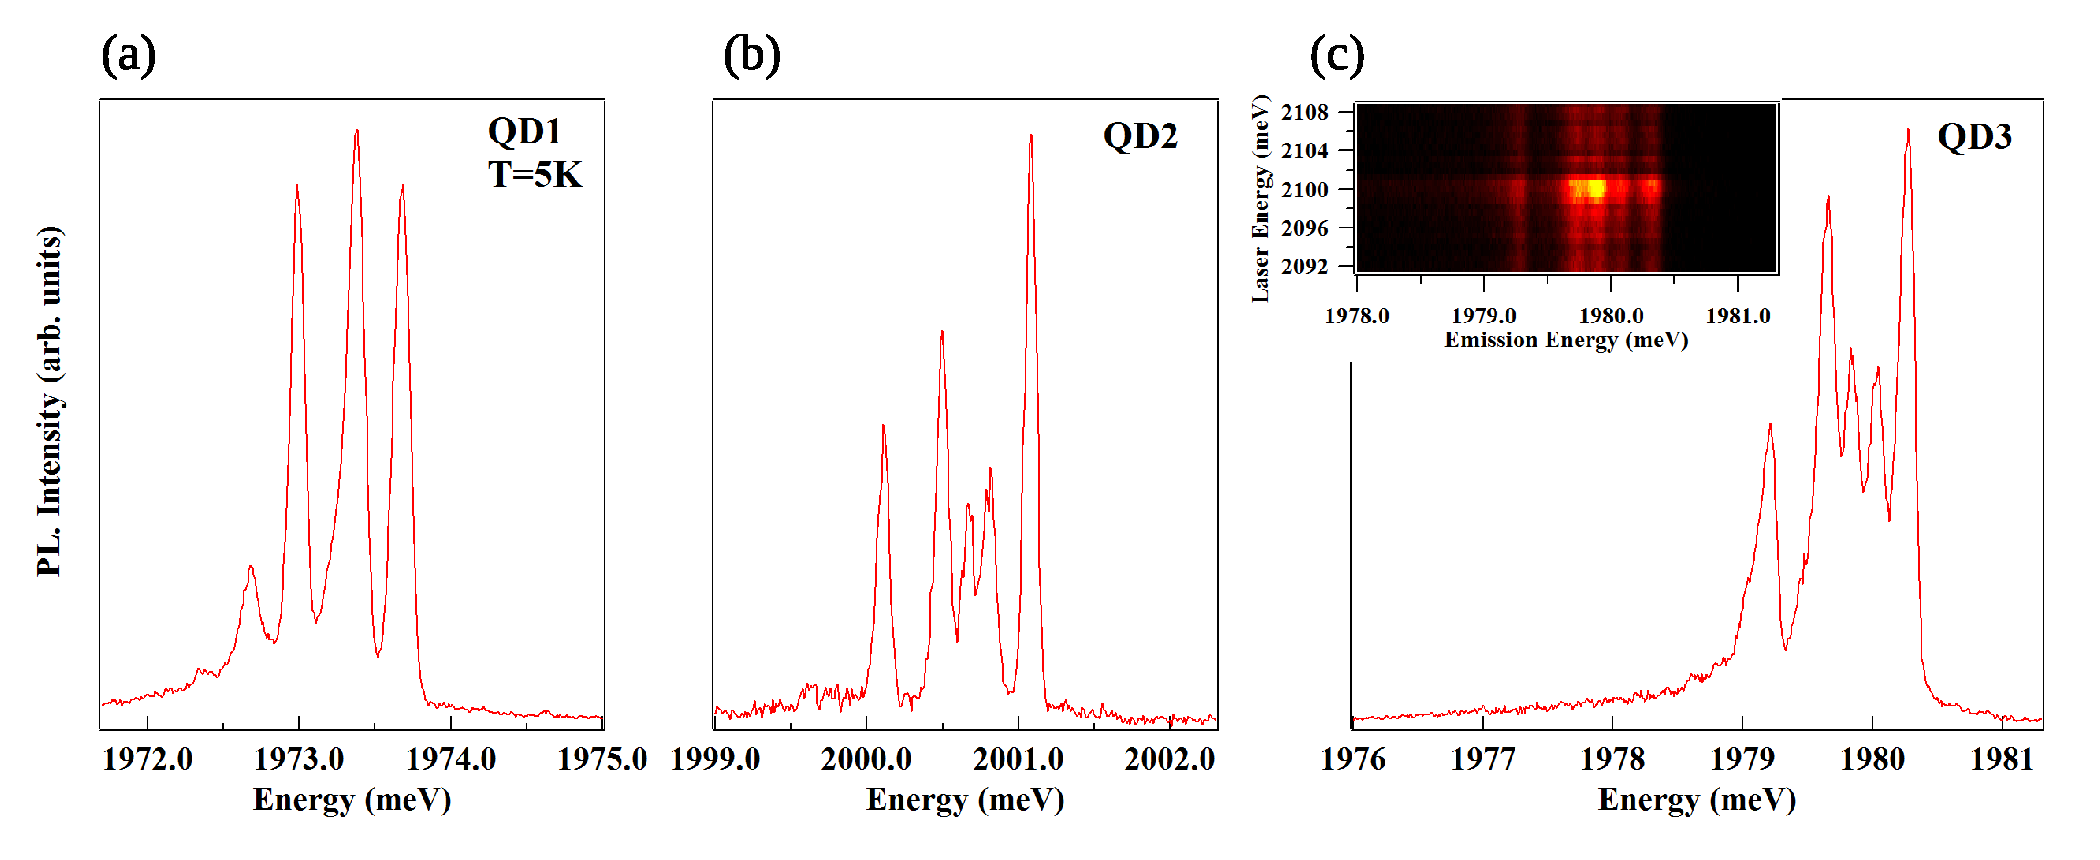
\includegraphics[width=15cm]{04-CrMagOpt/Pictures/Spectras.eps}
	\end{center}
	\caption{(a) PL of QD1 X-Cr complex at low temperature (T=5K). Inset presents the PLE map of this QD, showing a sharp quasi-resonant state for an excitation at 2100 meV. (b) PL of QD2 X-Cr complex at low temperature. (c) PL of QD3 X-Cr complex at low temperature.}
	\label{SpectraX}
	\end{figure}

	Low temperature (T=5K) PL of the neutral exciton (X-Cr) of several QD doped with a single Cr are reported in Fig.~\ref{SpectraX}. Four emission lines are observed as shown in QD3, with the central peak being split in some QDs, such as QD1 and QD2 spectra. Scanning with an energy tunable laser, we saw that all the peaks share a common quasi-resonant state, where all are at a maximum intensity, as highlighted in the inset of Fig.~\ref{SpectraX}(a). This is an indication that they originate from the same dot. Variations in the relative intensities of the peaks are observed in different dots. The lowest energy peak is shown as getting more intense  when the splitting of the central peak get wider.

\begin{figure}[h!]
	\begin{center}
		\includegraphics[width=10cm]{04-CrMagOpt/Pictures/EnLvl.png}
	\end{center}
	\caption{Illustration of the energy levels of the ground state (Cr), the bright exciton states ($|\pm1\rangle$) coupled to the spin of a Cr (X-Cr) and dominant PL transitions ($\sigma$+, $\sigma$-). The states $|$S$_z = \pm2\rangle$ cannot be populated through thermalization, and thus the recombination channel are not shown on this schema.}
	\label{CrEnergyStruct}
	\end{figure}

	In a II-VI semiconductor, the orbital momentum of the Cr connects the spin of the atom to its local strain environment through the modification of the crystal field and the spin-orbit coupling. For biaxial strain in the (001) plane, the ground state of a Cr spin is split by a strain induced magnetic anisotropy term ${\cal H}_{Cr,\varepsilon_\parallel}=D_0S^2_z$ (see chap.~\ref{CrSemiCon}). It was deduced from electron paramagnetic resonance of bulk Cr-doped CdTe that $D_0$ is positive for compressive biaxial strain~\cite{EPRCr}. In a self-assembled CdTe/ZnTe QD with large in-plane strain, the Cr spin energy levels are split with S$_z$=0 at low energy (Fig.~\ref{CrEnergyStruct}). A value of $D_0$ in the 1 meV range can be expected for a CdTe layer strained on a ZnTe substrate, as shown in chap.~\ref{CrSemiCon}.
	
	When an electron-hole (e-h) pair is injected in a Cr-doped QD, the bright excitons are split by the exchange interaction between the spins of Cr and carriers. In flat self-assembled QDs, the heavy-holes and light-holes are separated in energy by the biaxial strain and the confinement. In a first approximation, the ground state in such QD is a pure heavy-hole (J$_z$=$\pm$3/2) exciton and the exchange interaction with the Cr spin S is described by the spin Hamiltonian 
	\begin{eqnarray}
		{\cal H}_{c-Cr}=I_{eCr}\vec{S}\cdot\vec{\sigma}+I_{hCr}S_zJ_z
	\end{eqnarray}		
with $\vec{\sigma}$ the electron spin and J$_z$ the hole spin operator. I$_{eCr}$ and I$_{hCr}$ are, respectively, the exchange integrals of the electron and the hole spins with the Cr spin. These exchange energies depend on the exchange constant of the $3d$ electrons of the Cr with the carriers in CdTe and on the overlap of the Cr atom with the confined carriers. The exchange interaction of the Cr spin is ferromagnetic for both electron and hole spins in common II-VI semiconductors and a typical exchange constant 4 to 5 times larger for the holes than for the electrons is also expected in CdTe~\cite{DMSCrExchInt,CdCrSExchInt}.
	
	For highly strained CdTe/ZnTe QDs with a weak hole confinement, the strain induced energy splitting of the Cr spin $D_0S^2_z$ is much larger than the exchange energy with the confined carriers ($D_0\gg |I_{hCr}|>|I_{eCr}|$). The exchange interaction with the exciton acts as an effective magnetic field which further splits the Cr spins states S$_z$=$\pm$1 and S$_z$=$\pm$2. The resulting X-Cr energy levels are presented in Fig.~\ref{CrEnergyStruct}. The exciton recombination does not affect the Cr atom and its spin is conserved during the optical transitions. Consequently, the large strain induced splitting of the Cr spin is not directly observed in the optical spectra. However, at low temperature, the Cr spin thermalize on the low energy states S$_z$=0 and S$_z$=$\pm$1. This leads to a PL dominated by three contributions: a central line corresponding to S$_z$=0 and the two outer lines associated with S$_z$=$\pm$1 split by the exchange interaction with the carriers.

	\begin{figure}[h!]
	\begin{center}
		\includegraphics[width=15cm]{04-CrMagOpt/Pictures/LinPol.png}
	\end{center}
	\caption{(a) Low temperature (T=5K) PL of QD2 recorded in circular polarization: $\sigma +$ in blue and $\sigma -$ in red. (b) Low temperature PL of QD2 recorded along two orthogonal directions. (c) Linear polarization PL intensity map of QD2. The 0$^{\circ}$ polarization angle corresponds to an emission polarized along the QD cleavage axis, either $110$ or $1\bar{1}0$. (d) Illustration of the energy levels of the ground state (Cr), the bright exciton states ($|\pm1\rangle$) coupled to the spin of a Cr (X-Cr), showing the splitting of the central peak via the bright exciton coupling, and dominant PL transitions ($\sigma$+ (blue), $\sigma$- (red) and $\pi$ (green and black)).}
	\label{CrLinPolar}
	\end{figure}
	
	Cr-doped quantum dots exhibit a linear polarization dependence, as presented in Fig.~\ref{CrLinPolar}. The central line (S$_z$=0) is split and linearly polarized along two orthogonal directions. As in non-magnetic QDs, this results from a coupling of the two bright excitons $|\pm1\rangle$ by (i) the short range e-h exchange interaction in the presence of valence band mixing and/or (ii) the long-range e-h exchange interaction in a QD with an in-plane shape anisotropy~\cite{SplitInvTh}. This anisotropic e-h exchange energy mixes the bright exciton associated with the same Cr spin state, inducing an extra splitting between them. The mixing is maximum for the central pair of bright excitons (S$_z$=0) which are initially degenerated. The outer lines are also slightly linearly polarized but the influence of the e-h exchange interaction is attenuated by the initial splitting of the $|\pm1\rangle$ excitons induced by the exchange interaction with the Cr spin S$_z$=$\pm1$.	

	\begin{figure}[h!]
	\begin{center}
		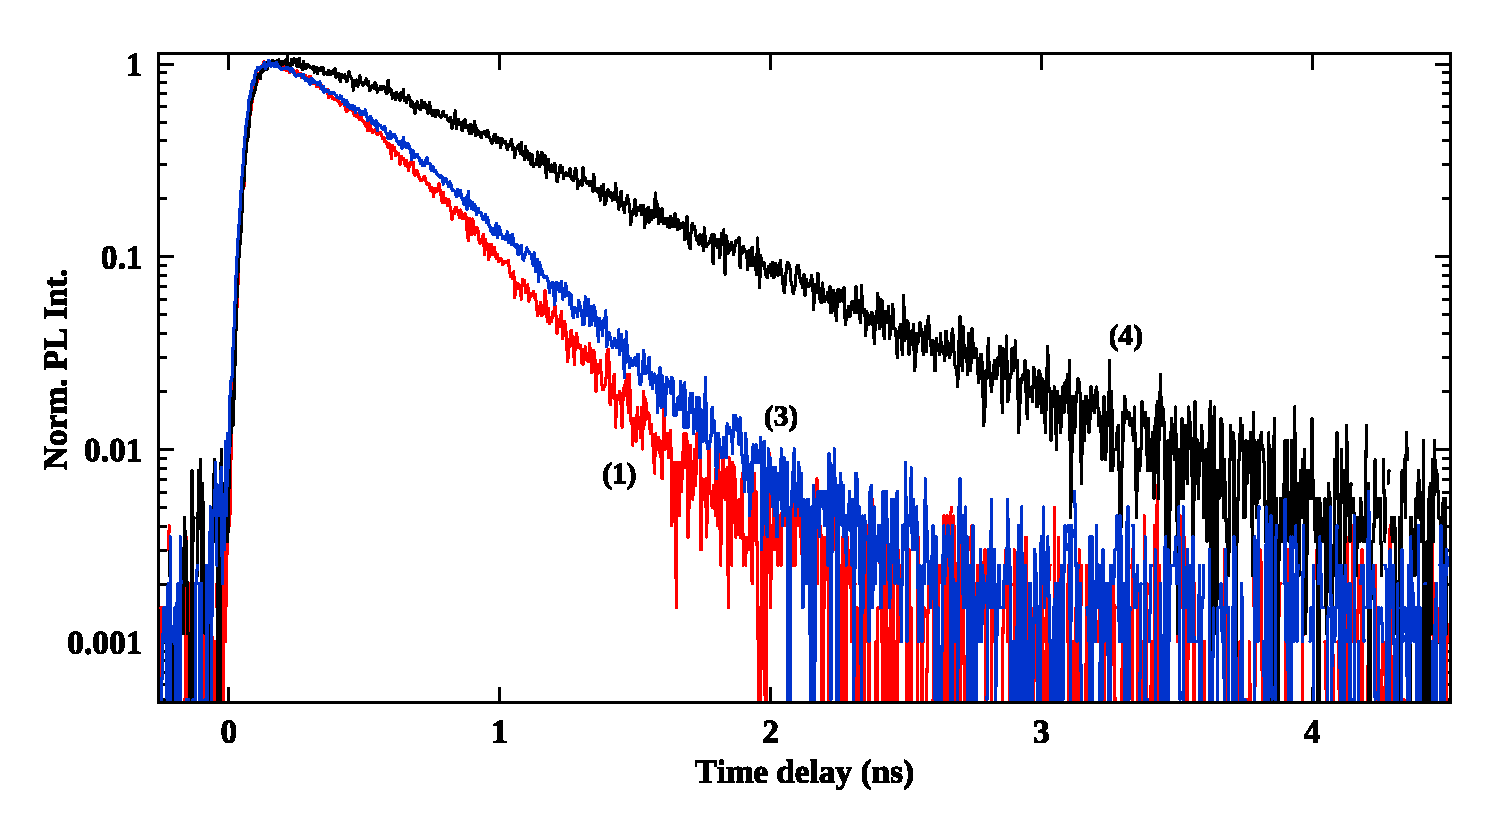
\includegraphics[width=10cm]{04-CrMagOpt/Pictures/Decay.eps}
	\end{center}
	\caption{Time resolved PL of QD2 taken on two exterior peaks, attributed to $|S_z = +1\rangle$ and $|S_z = -1\rangle$ (noted (1) and (3) in Fig.~\ref{CrLinPolar}(a)), and the lower energy one (noted (4)).}
	\label{CrDecay}
	\end{figure}

	In order to identify the lower energy peak ((4) in Fig.~\ref{CrLinPolar}(a)), we took the time resolved photoluminescence of the emission peaks, presented in Fig.~\ref{CrDecay}. One can notice that the line (4) present a decay time about twice as long as the high energy peak. A long recombination time is one of the characteristics of a dark exciton emission~\cite{DELongLifetime}. Under normal circumstances, the recombination of such a state is non-radiative. However, it is possible to observe a dark exciton recombination emitting a photon in low symmetry quantum dot~\cite{DELum}. This hypothesis will be confirmed by the magneto-optical study of the dot presented in Fig.~\ref{CrMagOptExp} and \ref{CrMagOptMod}.
	
	\begin{figure}[h!]
	\begin{center}
		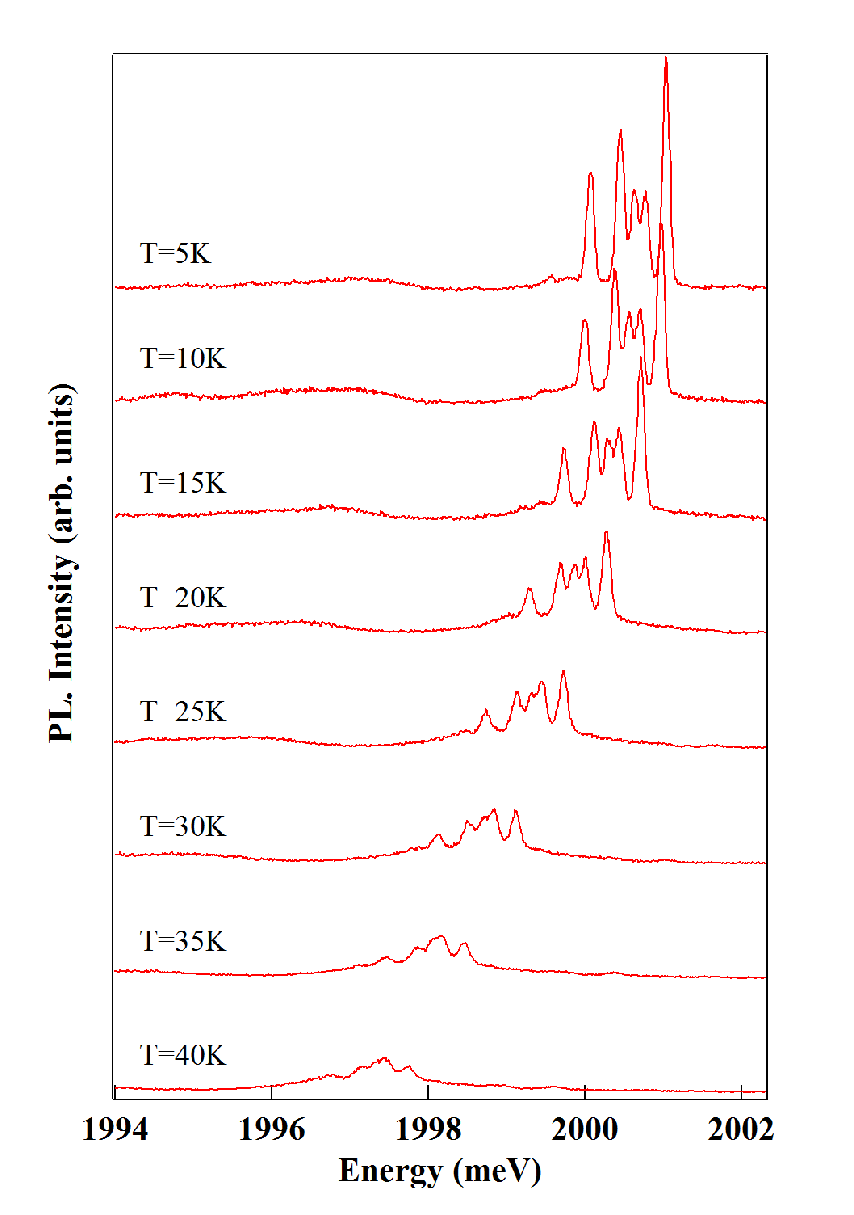
\includegraphics[width=7cm]{04-CrMagOpt/Pictures/Temp.eps}
	\end{center}
	\caption{Temperature evolution of QD2 PL, from T=5K to T=40K. The red shift and peak broadening are clearly visible. Even at 40K, $|$S$_z = \pm2\rangle$ states do not appear.}
	\label{CrTemp}
	\end{figure}	
	
	Since the absence of PL on $|\pm2\rangle$ is linked to their impossibility to be thermally populated, one could expect to see their emission at higher temperature. Fig.~\ref{CrTemp} presents the dot PL at several temperatures. With the increase of the temperature, we observe a significant line broadening induced by the interaction with acoustic phonons. In order to keep a significant PL intensity and resolved PL lines, we limited our investigation to temperature below 50K. No contribution of the $|$S$_z$=$\pm2\rangle$ Cr spins states are observed in the emission of the exciton.
		


		\subsection{Excited states of a Cr-doped QD}
			
	\begin{figure}[h!]
	\begin{center}
		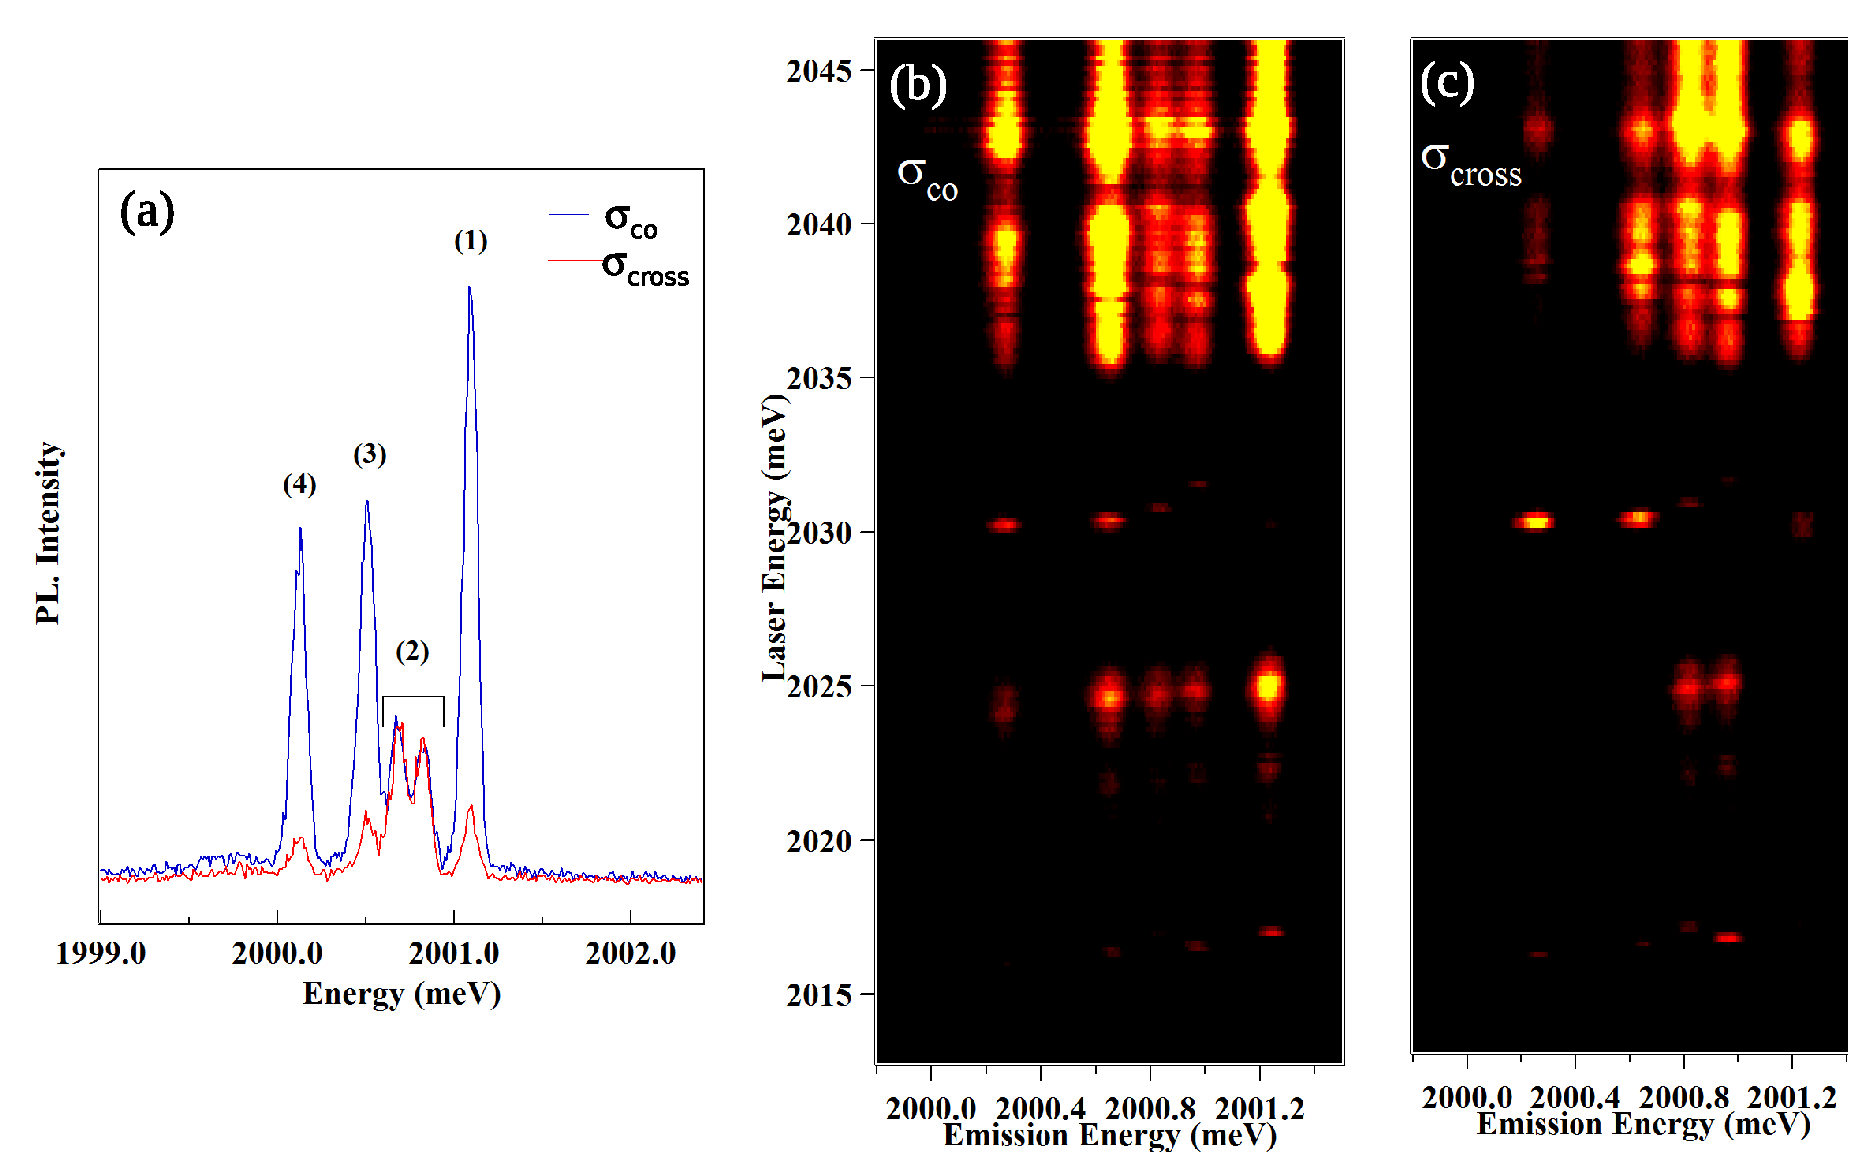
\includegraphics[width=10cm]{04-CrMagOpt/Pictures/PLEDotPres.eps}
	\end{center}
	\caption{(a) PL spectra of the exciton in QD2 (X-Cr) for co- and cross-circularly polarized excitation/detection [À VÉRFIER : taken on the 2175 meV quasi-resonant state]. (b) QD2 X-Cr PLE map in $\sigma$- polarization. Several excited states are identifiable and are discussed in Fig.~\ref{PLEClose} and \ref{PLE2030}.}
	\label{PLEDotPres}
	\end{figure}

	In order to study the different excited states presented by a QD doped with a single Cr atom, we took the PLE of QD2 starting close the dot. The dot spectra is presented in Fig.~\ref{PLEDotPres}(a) in both $\sigma$ polarizations. The central peaks do not show dependency in circular polarization, which is coherent with their linear polarization dependency presented in Fig.~\ref{CrLinPolar}(a) and (b). The excitation laser is $\sigma$+ polarized in order to control the spin of the injected exciton. The exterior peaks emission being in $\sigma$+ polarization shows that there is no spin flip of the exciton before recombination.
	
	Fig.~\ref{PLEDotPres}(b) presents the entire PLE of QD2 X-Cr complex. However, one can note several other excited states along the scan. In this section, we will discuss several of them.
	
	\begin{figure}[h!]
	\begin{center}
		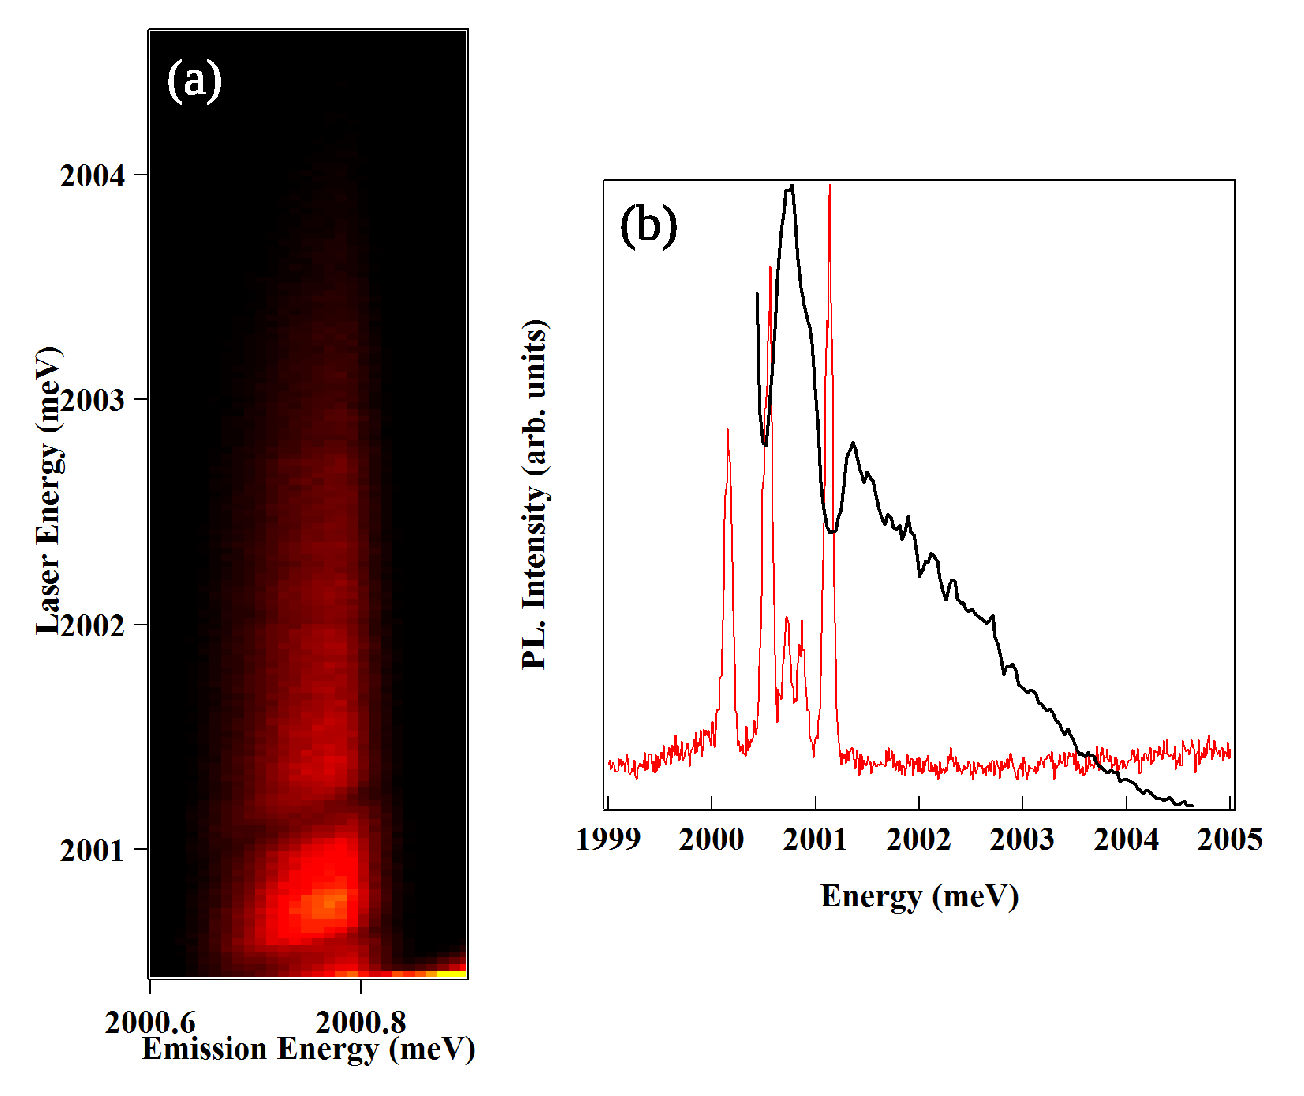
\includegraphics[width=10cm]{04-CrMagOpt/Pictures/PLEClose.eps}
	\end{center}
	\caption{(a) PLE scan of the lower energy peak, taken close to the QD emission energy, showing the phonon replica taken in $\pi$ detection. The emission integrated intensity in function of the laser energy is plotted in (b) (black curve) along with the PL spectra of QD2 taken in $\sigma$+ polarization.}
	\label{PLEClose}
	\end{figure}
	
	The first remarkable feature of this scan is the really long luminescence of the acoustic phonon replica. As shown on the zoom in Fig.~\ref{PLEClose}(a), the probed peak continues to emit with an excitation several millielectronvolt above the excited state, remaining visible until 2004 meV. One can also see two sharp intensity diminutions in this emission. Mapping the intensity of this peak emission to the quantum dot spectrum (Fig.~\ref{PLEClose}(b)), it is evidenced that these diminutions occur when the laser is in resonance with a QD emission line. The absorption then preferentially occurs in this resonantly excited state than in the acoustic phonon band.
	
	\begin{figure}[h!]
	\begin{center}
		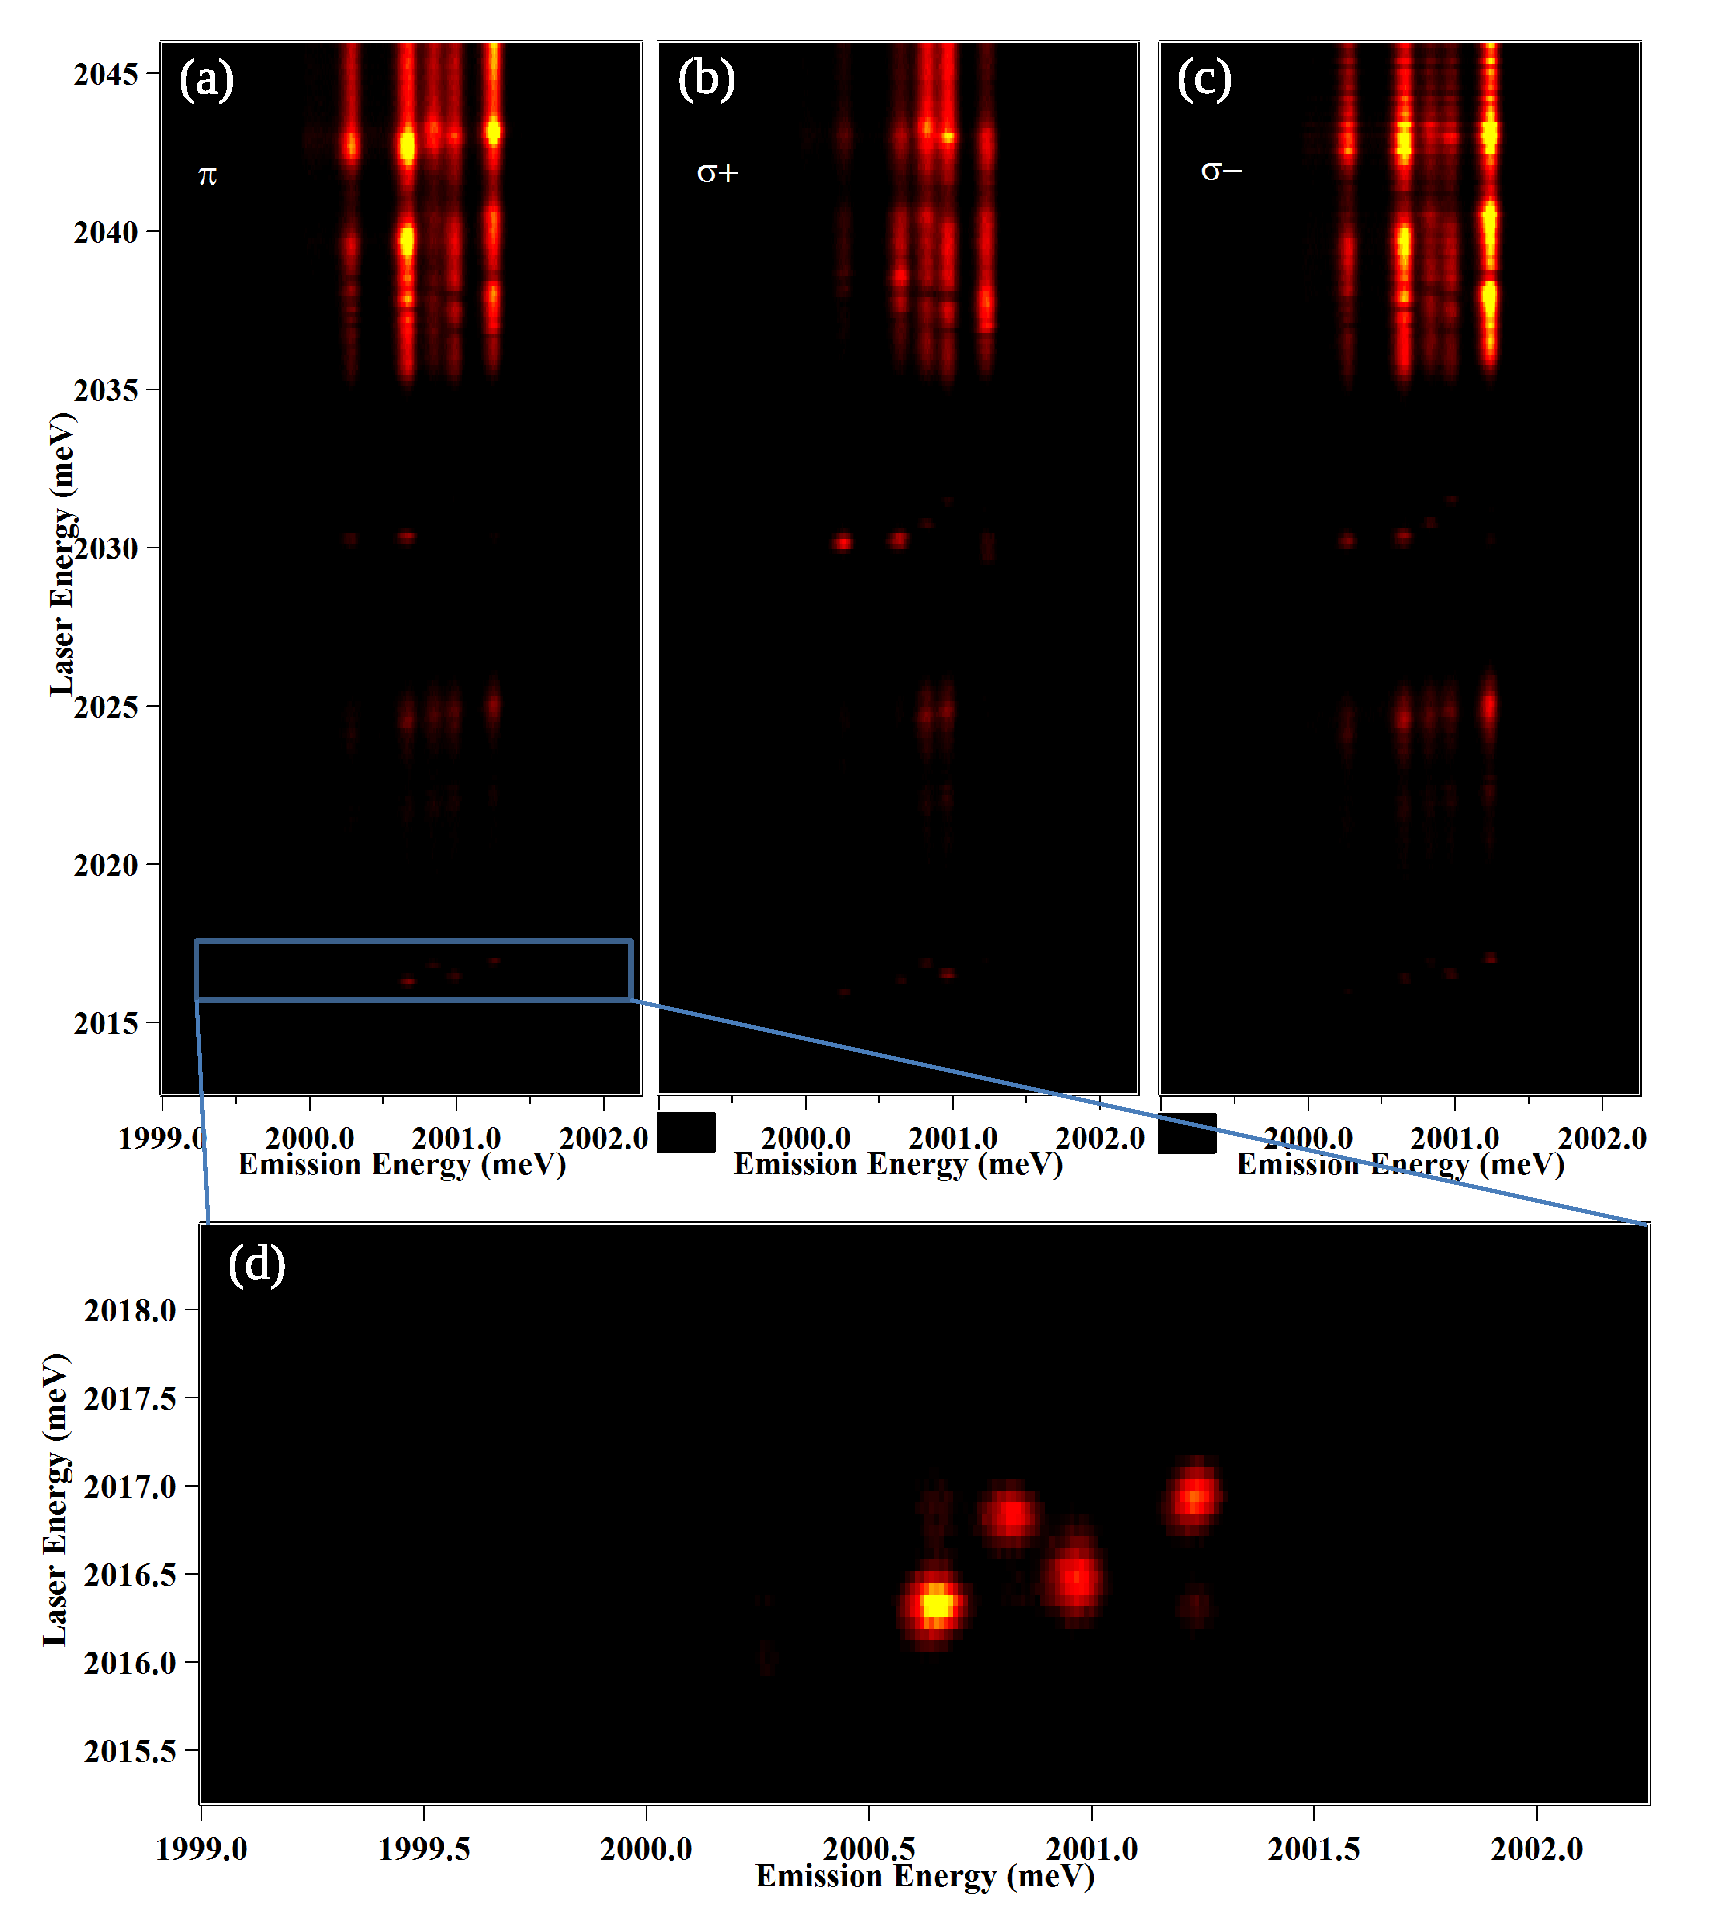
\includegraphics[width=12cm]{04-CrMagOpt/Pictures/PLE2030.eps}
	\end{center}
	\caption{(a) - (c) PLE map between 2046 meV and 2013 meV presenting several excited, detecting in $\pi$ (a),  $\sigma +$ (b) and $\sigma -$ (c). (d) Zoom in a particular excited state presented a splitting inversion, taken in $\pi$ detection.}
	\label{PLE2030}
	\end{figure}
	
	At higher excitation energy, several excited states appear. The lower energy one is around 2018.5 meV, zoomed in on Fig.~\ref{PLE2030}(d). On this excited state, each peak presents a slightly different resonant energy. One can see that the order of appearance of the two central peaks seems to be reversed compared to the external ones. This phenomenon was first observed on QDs in GaAs quantum well~\cite{FineStructSplitGaAsdots}. This indicates an inversion of the splitting due to electron-hole exchange interaction~\cite{SplitInvTh}.
	
	Another excited state can be saw at 2025 meV. This excited state occurs on a large energy band and can be linked back to an excitation to the optical phonon. Looking at the $\sigma$ polarized emission of this state (Fig.~\ref{PLE2030}(b) and (c)), we can see that this excitation presents a really good spin conservation: the low and high energy peaks are strongly $\sigma$ polarized, while the central peaks do not show dependency over circular polarization. This, once again, show the good spin conservation of the system, as highlighted on the quasi-resonant state. 
	
	Finally, another interesting excited state appear at 2030 meV. This state presents an exchange-induced splitting  different from the splitting in the quasi-resonant state. This is due to a difference in the carriers and Cr atom wavefunction overlap. One can also noticed the this state presents a stronger luminescence in $\sigma_{cross}$ than in $\sigma_{co}$, [TO REDISCUSS] hinting at a spin flip of the hole before the recombination.
		
		\subsection{Magneto-optics of a quantum dot doped with a single Cr}
		
	The structure of the energy levels in Cr-doped QDs is confirmed by the evolution of the PL spectra in magnetic field (up to 11T) in Faraday configuration~\cite{BesombesPumpMnSFD}, presented in Fig.~\ref{CrMagOptExp}. One can see that the Zeeman energy of the exciton under magnetic field can compensate the exciton splitting induced by the exchange interaction with the Cr~\cite{LegerQDGeomEffect}. For QD3, this results in an anti-crossing of $|+1\rangle$ and $|-1\rangle$ excitons due to the e-h exchange interaction around B$_z$=6 T observed both in $\sigma$+ and $\sigma$- polarizations (anti-crossing (2) and (3) in Fig.~\ref{CrMagOptExp}(a)).
		
	\begin{figure}[h!]
	\begin{center}
		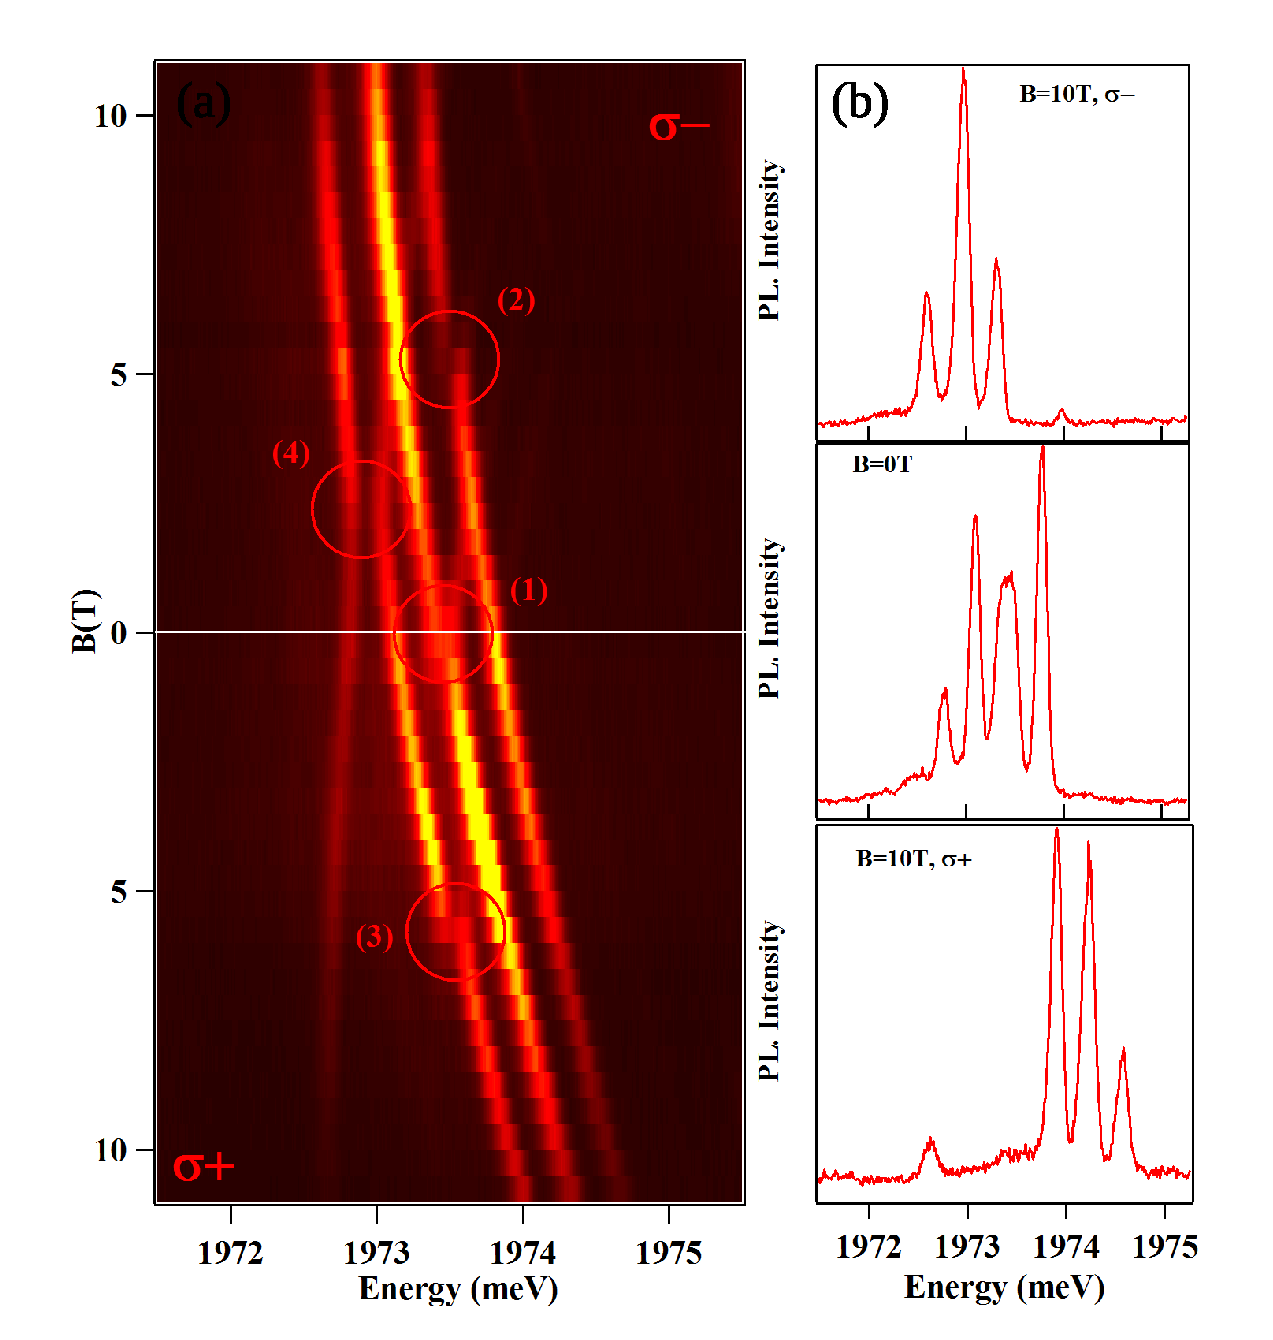
\includegraphics[width=10cm]{04-CrMagOpt/Pictures/MagOptv2.eps}
	\end{center}
	\caption{(a) Circularly polarized X-Cr PL evolution under magnetic field (B$_z$) in QD3. Noticeable anti-crossing  are highlighted and numbered. (b) QD3 X-Cr PL spectra taken at 0 and $\pm10$T.}
	\label{CrMagOptExp}
	\end{figure}
		
		The low energy emission presented as a dark exciton in Fig.~\ref{CrDecay} shows an anti-crossing with the bright excitons under B$_z$ in $\sigma$- polarization (anti-crossing (4) in Fig.~\ref{CrMagOptExp}). As illustrated in Fig.~\ref{CrMagOptMod}(b), this anti-crossing arises from a mixing of the bright and dark excitons interacting with the same Cr spin state. Observed in $\sigma$- polarization, it corresponds to the mixing of the exciton states $|-1\rangle$ and $|+2\rangle$ coupled to the Cr spin S$_z$=-1. This dark/bright excitons coupling $\delta_{12}$ is induced by the e-h exchange interaction in a confining potential of reduced symmetry (lower than C$_{2v}$)~\cite{DERecombTh}. In such symmetry, the dark exciton acquire an in-plane dipole moment which lead to possible optical recombination at zero magnetic field~\cite{DELum} as observed in these QDs. The oscillator strength of this "dark exciton" increases as the initial splitting between $|-1\rangle$ and $|+2\rangle$ excitons is reduced by the magnetic field (Fig.~\ref{CrMagOptMod}(b)).
		
		\begin{figure}[h!]
	\begin{center}
		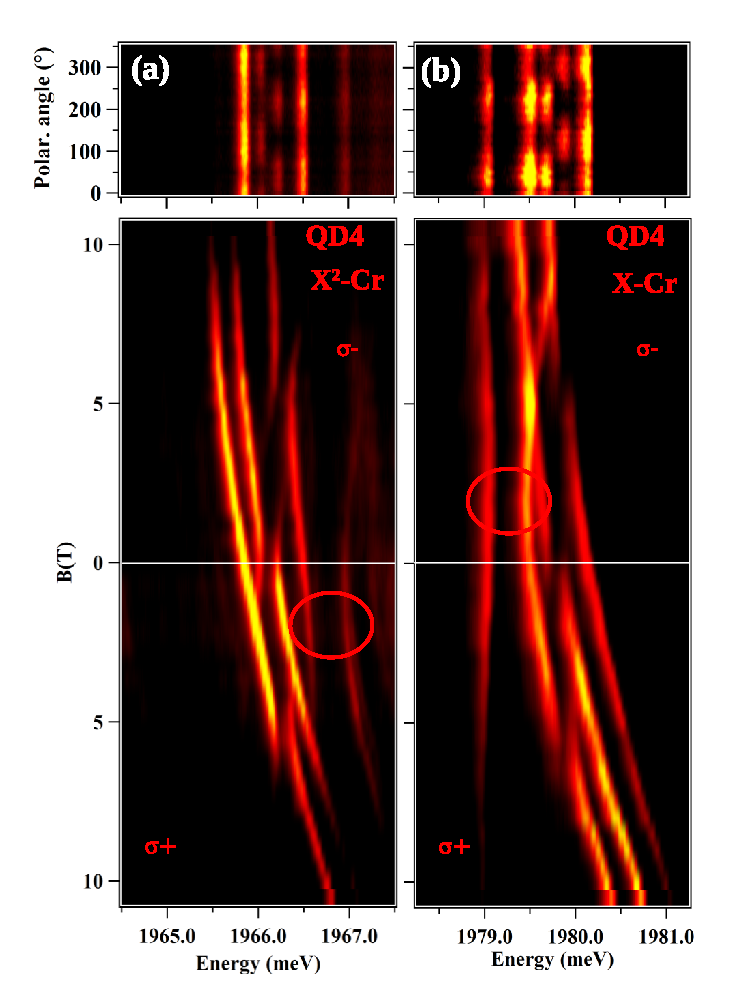
\includegraphics[width=10cm]{04-CrMagOpt/Pictures/MagOptLowSym.eps}
	\end{center}
	\caption{Linear polarization intensity map (top panel) and intensity map of the longitudinal magnetic field dependence of the emission (bottom panel) of (a) X$^2$-Cr and (b) X-Cr in QD3.}
	\label{CrMagOptLowSym}
	\end{figure}
		
		To illustrate the influence of the QD symmetry on the magneto-optical properties of X-Cr, we show in Fig.~\ref{CrMagOptLowSym}(b) the emission of a QD with a different strain state (QD4). For QD3, the splitting of the central peak is not clear in the PL at 0T (Fig.~\ref{SpectraX}(a)) without the linear polarization map, while two linearly polarized peaks appears clearly in QD4 spectra. This difference in emission arise from a difference in the in-plane strain of each QD~\cite{SplitInvTh}. The dark exciton emission is also stronger in QD2, confirming a lower symmetry than QD3.
		
		Investigating both the biexciton and the exciton in the same Cr-doped QD, we can also analyze the impact of the carrier-Cr interaction on the fine structure of the Cr spin. The magnetic field dependency of X$^2$-Cr emission in QD2 is presented along with the X-Cr emission as a contour plot in Fig.~\ref{CrMagOptLowSym}(a) and (b) respectively. The PL under magnetic field of X-Cr and X$^2$-Cr present a mirror symmetry. In particular, the dark/bright exciton mixing observed around B$_z$=2.5T on the low energy side of the PL in $\sigma-$ polarization for X-Cr is observed on the high energy side in $\sigma+$ polarization for X$^2$-Cr (circles in Fig.~\ref{CrMagOptLowSym}(a) and (b)).
		
		If one consider the ground state of X$^2$ as a spin-singlet (total spin 0), it cannot be split by the magnetic field or the spin interaction part of the carriers-Cr Hamiltonian. The creation of two excitons in the QD cancels the exchange interaction with the Cr atom. Thus, the PL of  X$^2$-Cr is controlled by the final state of the optical transitions, i.e. the eigenstates of X-Cr, resulting in the observed mirror symmetry in the PL spectra. However, in some of the QDs, the X$^2$-Cr emission slightly deviates from this simple picture: a smaller energy splitting is observed for X$^2$-Cr compared to X-Cr (see X-Cr and X$^2$-Cr in Fig.~\ref{CrMagOptLowSym}). This shows that there is an interaction of X$^2$ with the Cr atom. It could result from a perturbation of the carriers' wave function by the interaction with the magnetic atom~\cite{CarInSpinSplit,BiexFinStruct} or a modification the local electric field which controls the Cr fine structure. [TO BE INVESTIGATED]
		
	\section{Modelization of a Cr-doped QD\label{QDParam}}
		
	\begin{figure}[h!]
	\begin{center}
		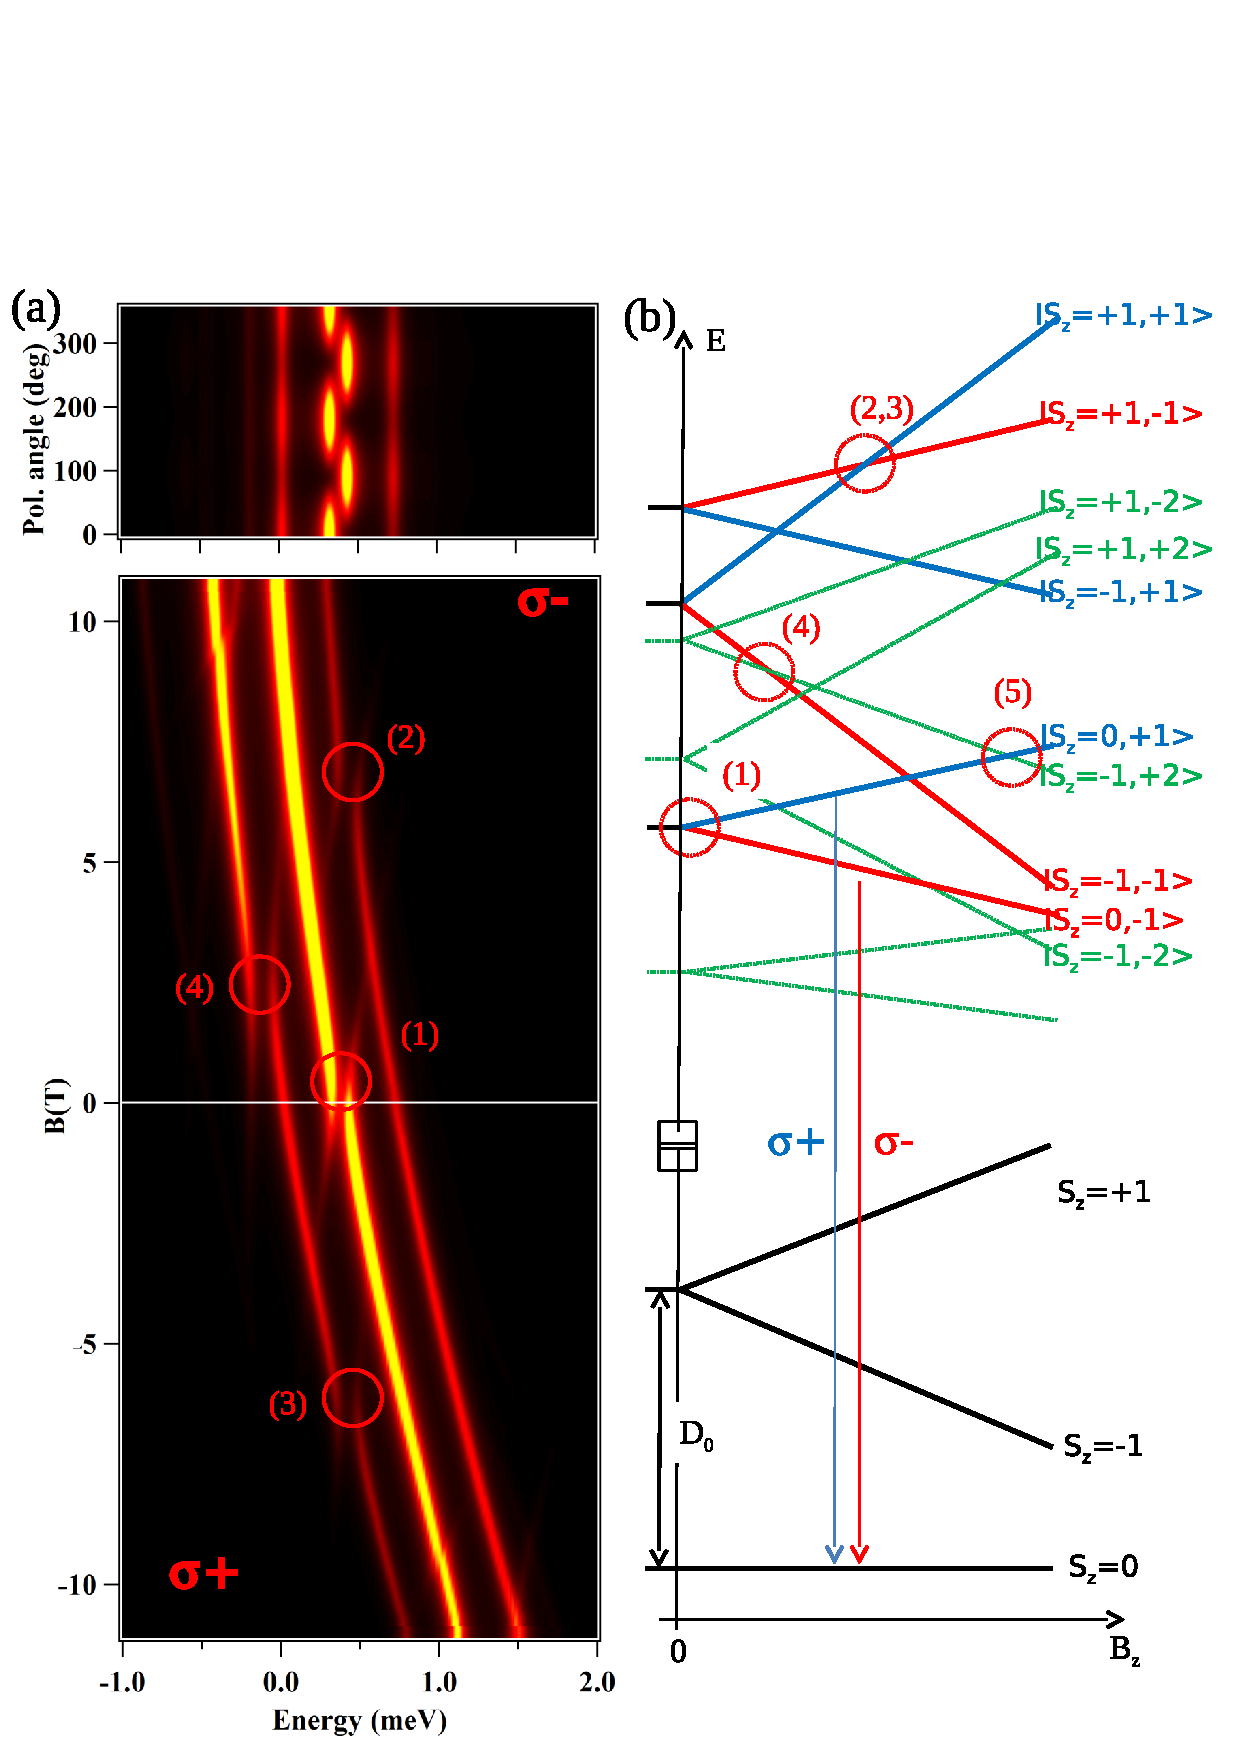
\includegraphics[width=10cm]{04-CrMagOpt/Pictures/SimulMagOptv2.png}
	\end{center}
	\caption{(a) Up: Calculated linear polarization PL intensity map of X-Cr at zero field. The 0$^{\circ}$ polarization angle correspond to an emission polarized along the $100$ axis. Down: Calculated X-Cr circularly polarized magnetic field dependency. Details of the model and parameters are listed in Tab.~\ref{CrModelParam}. Corresponding anti-crossing are highlighted in same fashion as on Fig.~\ref{CrMagOptExp}. (b) Schema of the magnetic field dependency of the energy levels of the low energy Cr spin states S$_z$=0 and S$_z$=$\pm$1, and corresponding bright ($|+1\rangle$ blue, $|-1\rangle$ red) and dark ($|\pm2\rangle$ green) X-Cr energy levels.}
	\label{CrMagOptMod}
	\end{figure}
	
	We calculated the magneto-optic behaviour of Cr-doped QDs by diagonalizing the complete Hamiltonian of the e-h-Cr in self-assembled dots. This hamiltonian can be separated as follows:
	
	\begin{eqnarray}
\label{X-Cr} {\cal H}_{X-Cr}={\cal H}_{Cr,\varepsilon}+{\cal H}_{c-Cr}+{\cal H}_{mag}+{\cal H}_{e-h}+{\cal H}_{band}+{\cal H}_{scat}
\end{eqnarray}
where:

${\cal H}_{Cr,\varepsilon}$ describes the fine structure of the Cr atom and its dependency on local strain, as presented in Eq.~\ref{Cralone}. It is mainly drived by D$_0$, the magnetic anisotropy. E, the in-plane strains, also appears in this Hamiltonian, but have to be kept small in order to model the found dots (see Fig.~\ref{CrHighE} for the emission of a dot with a higher E).

${\cal H}_{c-Cr}$ describes the coupling of the electron and hole with the Cr spin, depending on I$_{eCr}$, the exchange integral of the electron-Cr spins, and I$_{hCr}$, the exchange integral of the hole-Cr spins, as described in Eq.~\ref{HcCr}.

${\cal H}_{mag}$ describes the effect of an exterior magnetic field, coupled to both the Cr and carrier spins by the Zeeman terms, depending on the $g$-factor of each of them, and including the diamagnetic shift of the electron-hole  via the term $\gamma$.
\begin{eqnarray}
	{\cal H}_{mag} = g_{Cr}\mu_B\overrightarrow{B}.\overrightarrow{S}+g_{e}\mu_B\overrightarrow{B}.\overrightarrow{\sigma}+g_{h}\mu_B\overrightarrow{B}.\overrightarrow{J}+\gamma B^2
\end{eqnarray}

${\cal H}_{e-h}$ describes the short range and long range electron-hole interaction, through the bright and dark exciton splitting $\delta_0$, the bright exciton coupling $\delta_1$, the dark exciton coupling $\delta_2$ and the bright and dark exciton coupling $\delta_{11}$ and $\delta_{12}$. All of these term are described in Eq~\ref{Ieh}.

${\cal H}_{band}$, the band Hamiltonian, presented in Eq.~\ref{HBand}, stands for the energy of the electrons (i.e. the band gap energy E$_g$), and the heavy-holes (hh) and light-holes (lh) energies, depending on the splitting between lh and hh $\Delta_{lh}$, and the anisotropy of the QD.

${\cal H}_{scat}$ describes the perturbation of the wave function of the exciton in the initial state of the optical transition by the hole-Cr exchange interaction, controlled by the parameter $\eta$. This perturbation depends on the value of the exchange energy between the Cr spin S$_z$  and the hole spin J$_z$ and can be represented, using second order perturbation theory, by an effective spin Hamiltonian \cite{CarInSpinSplit,BiexFinStruct,DynhMn}
\begin{eqnarray}
{\cal H}_{scat}=-\eta S_z^2
\end{eqnarray}
\noindent with $\eta>0$.

	We considered the general case of QDs with a symmetry lower than C$_{2v}$ (truncated ellipsoidal lens for instance~\cite{DERecombTh}), and took into account the influence of this reduced symmetry on the valence band and on the e-h exchange interaction. The population of the X-Cr spin states split by the large magnetic anisotropy and the carriers-Cr exchange interaction is described by a spin effective temperature T$_{eff}$. The results of the model obtained with T$_{eff}$=25K, D$_0$=2.5 meV and an electron-Cr (hole-Cr) exchange interaction I$_{eCr}$=-70$\mu$eV (I$_{hCr}$=-280 $\mu$eV) are reported in Fig.~\ref{CrMagOptMod} (parameters not specific to Cr-doped QDs are listed in Tab.~\ref{CrModelParam}). Such parameters do not aim to fit the data and are only reasonable order of magnitude. The PL of X-Cr at zero field and its evolution in magnetic field can be qualitatively reproduced. In particular, the description of the spin states occupation by T$_{eff}$ is sufficient to reproduce the observed emission from the three low energy X-Cr levels (Cr spin states S$_z$=0 and S$_z$=$\pm$1). The splitting of the central line at zero field (anti-crossing (1)) and the anti-crossings under magnetic field (anti-crossings (2) and (3) around B$_z$=6T for the Cr spin states S$_z$=+1 and anti-crossings (4) with the dark exciton around B$_z$=2T) are also well reproduced by the model.
	
	


\begin{table}[t] \centering
	\caption{Values of the parameters used in the model of Cr-doped CdTe/ZnTe quantum dot presented in Fig.~\ref{CrMagOptMod}. The value of the parameters not listed in the table is 0. The chosen values are typical for CdTe/ZnTe quantum dots and can be compared with parameters extracted from Mn-doped quantum dots \cite{DynhMn,VBM}. These values are reasonable to reproduce the emission of the QDs presented in this thesis.}
	\begin{tabular}{p{0.9cm}p{0.9cm}p{0.9cm}p{0.9cm}p{0.9cm}p{0.9cm}p{0.9cm}p{0.9cm}}
\hline\hline
I$_{eCr}$ & I$_{hCr}$ & $\delta_0$ & $\delta_1$ & $\delta_{12}$ & $\delta_{11}$ & $\frac{|Q|}{\Delta_{lh}}$ & $\frac{|R|}{\Delta_{lh}}$ \\
$\mu eV$ & $\mu eV$ & $meV$ & $\mu eV$ & $\mu eV$ & $\mu eV$ &  & \\
\hline
-70 & -280 & -1 & 250 & 150 & 50 & 0.05 & 0.05 \\
\hline\hline 
	\end{tabular}
	\begin{tabular}{p{0.9cm}p{0.9cm}p{0.9cm}p{0.9cm}p{0.9cm}p{1.3cm}p{0.9cm}p{0.9cm}}
arg(R) & $D_0$ & $g_{Cr}$ & $g_{e}$ & $g_{h}$ & $\gamma$ & $\eta$ & $T_{eff}$ \\
 & $meV$ & &  &  & $\mu eV/T^2$ & $\mu eV$ & K \\
\hline
$-\frac{\pi}{2}$ & 2.5 & 2 & -0.7 & 0.4 & 1.5 & 25 & 25 \\
\hline\hline
	\end{tabular}
	\label{CrModelParam}
	\end{table}
	
	The magnetic anisotropy D$_0$ cannot be precisely extracted from the PL spectra. However, a higher value would produce a smaller PL intensity of the sates S$_z$=$|\pm1\rangle$ than observed experimentally. In addition, for D$_0$ $<$ 2.25 meV, an anti-crossing due to an electron-Cr flip-flop controlled by I$_{eCr}$, labelled (5) in Fig.~\ref{CrMagOptMod}(c), would appear below B$_z$=11T on the central line in $\sigma$+ polarization.
	
	Having shown that our model reproduce well the evolution of the emission under variations of different parameters, we can run it to see the influence of E on the emission. This simulation was done by applying a small magnetic anisotropy D$_x$ along the $x$ axis of the quantum dot and none along the $y$ axis (D$_y$=0), creating an effective E. Results of such a study are presented on Fig.~\ref{CrHighE}, (a) and (b) for the X-Cr system, and (c) and (d) for the X$^c$-Cr one.
	
	\begin{figure}[h!]
	\begin{center}
		\includegraphics[width=10cm]{04-CrMagOpt/Pictures/HighE.eps}
	\end{center}
	\caption{For a QD with a small magnetic anisotropy along the $x$ axis (D$_x$ = 150 $\mu$eV, D$_y$ = 0 $\mu$eV,  D$_z$ = 2500 $\mu$eV): (a) calculated X-Cr linear polarization PL intensity at 0T; (b) calculated X-Cr circularly polarized magnetic field dependency; (c) calculated X$^c$-Cr linear polarization PL intensity at 0T; and (d) calculated X$^c$-Cr circularly polarized magnetic field dependency.}
	\label{CrHighE}
	\end{figure}
	
	The X-Cr map in linear polarization presents a dependency on all the three peaks at 0T, when only the central  peaks exhibit this behaviour in dots with a small in-plane anisotropy at the Cr position. The effect of such an anisotropy is to coupled to spin levels separated by two spin units, such as $|S_z = -1\rangle$ and $|S_z = +1\rangle$. This induce a mixing between two bright exciton states, leading to a linearly polarized emission. For a low E value, the strain induced splitting of $|S_z = \pm 1\rangle$ is high enough to strongly reduce the mixing of the exciton states. A higher in-plane strain anisotropy is able to couple the spin level and induced the linearly polarized emission.

	
	As can be expected, X$^c$-Cr doesn't present any linear polarization dependency, as shown on Fig.~\ref{CrHighE}(c).
	
	The evolution of the emission under magnetic field also presents different characteristics than a QD with magnetic anisotropy purely along z. Fig.~\ref{CrHighE}(b) presents the evolution in B of the X-Cr emission. 
One can note anti-crossings at +5T appearing on both $|S_z = +1\rangle$ and $|S_z = -1\rangle$, as well as an anti-crossing at -5T appearing on the low energy emission lines. These are similar to the anti-crossing (2), (3) and (4) on Fig.~\ref{CrMagOptMod}. Around 0T, other anti-crossings appear, on all the three peaks this time. Anti-crossing on the central peaks is the same as the anti-crossing (1) in Fig.~\ref{CrMagOptMod}. The ones appearing on the $|S_z = \pm 1\rangle$ peaks arise from the exciton mixing via E, as evidenced by the linear polarization.

	X$^c$-Cr in dot with high in-plane anisotropy at the Cr position also presents anti-crossing for a magnetic field around 1T, as shown in Fig.~\ref{CrHighE}(d). This anti-crossing appears when the Zeeman effect of the Cr atom compensates the electron-Chromium interaction and the hole-Chromium interaction.
				
	
	\section{Charge fluctuation of a Cr ion  in the vicinity  of the QDs}
	
	Some dots were found presenting a linear polarization dependency both on their central peaks and on their exterior peaks. However, such dots didn't present any anti-crossing when probed under magnetic field. Results of these experiments are presented in Fig.~\ref{CrSixPeaksMagOpt}.
	
	\begin{figure}[h!]
	\begin{center}
		\includegraphics[width=15cm]{04-CrMagOpt/Pictures/6peaks.eps}
	\end{center}
	\caption{(a) QD4 linearly polarized PL intensity at zero magnetic field. (b) and (c) Respectively X$^2$-Cr and X-Cr linear polarization PL dependence at zero magnetic of this QD. Both central and exterior peaks present linear polarization dependencies in this dots. (c) X-Cr magnetic field PL dependence on this QD. Zoom in presents anti-crossing appearing at B=9T.}
	\label{CrSixPeaksMagOpt}
	\end{figure}
	
	A common feature of all of these dots is the thin and well split X$^+$-Cr PL structure, shown on Fig.~\ref{CrSixPeaksMagOpt}(a) around 1949mev. X-Cr and X$^2$-Cr also present three well defined peaks, with a broad emission. This is not a general case, as some dots were found presenting a broad emission on X-Cr and X$^2$-Cr positions, such as QD6 presented in Fig.~\ref{CrSixPeaksSplit}. The linear polarization map of the PL of QD4 reveals that each peak presents a linear polarization dependency (Fig.~\ref{CrSixPeaksMagOpt}(b) and (c)).
	
	The PL evolution of such a dot is presented in Fig.~\ref{CrSixPeaksMagOpt}(d). The  diamagnetic shift is clearly visible. However, the only anti-crossings appear at B=9T for all the peaks (zoom in Fig.~\ref{CrSixPeaksMagOpt}(d)). Such anti-crossings are characteristic of an exciton in a QD with no magnetic atom: it arise from the dark and bright exciton mixing.
	
	\begin{figure}[h!]
	\begin{center}
		\includegraphics[width=12cm]{04-CrMagOpt/Pictures/EfieldX-Xc.eps}
	\end{center}
	\caption{(a) QD5 whole PL evolution under application of a bias voltage. (b) Zoom on X$^c$-Cr circular polarization PL intensity evolution under electric field. A strong stark shift is observed, as well as variation in the splitting. (c) Schema of the Schottky gate used to apply the bias voltage on the sample.}
	\label{CrSixPeaksEFieldX+}
	\end{figure}	
	
	In order to get more informations on these dots, it was decided to study them applying a bias voltage. The application of an electric field was realized via a sample with a Schottky gate in the same fashion than the one in chap.~\ref{ChargeSelec}. The resulting map is presented in Fig.~\ref{CrSixPeaksEFieldX+}(a). The first visible feature is the strong electric field dependency of the emission energy, more marked for X-Cr than for the X$^c$-Cr systems. The emission energy variation of the X-Cr complex occur on a 2.9 meV scale.
	
	There is another remarkable point on these maps, evidenced on the X$^+$-Cr complex on the Fig.~\ref{CrSixPeaksEFieldX+}(b): the splitting between each peak is changing with the applied electric field. The splitting between the high and low energy peaks varies from 0 meV for an applied bias voltage of -12V (no splitting) to 0.76 meV for 13V applied. This disappearance of the splitting for a certain bias voltage indicates that the overlap between the electron and the hole wave functions is changed by the application of an exterior electric field, to the point where they don't overlap at all.

	\begin{figure}[h!]
	\begin{center}
		\includegraphics[width=12cm]{04-CrMagOpt/Pictures/SplitUnderEfiledXCr.eps}
	\end{center}
	\caption{All these measures were taken on QD6 X-Cr complex at low temperature. (a) PL intensity dependency in linear polarization. In order to have the best contrast, the map was taken at -2.5V bias voltage. (b) Circular PL intensity evolution in electric field. A splitting began to appear around -2V of applied bias voltage. (c)-(d) Circular PL for an applied bias voltage of, respectively, 0V and -2.5V.}
	\label{CrSixPeaksSplit}
	\end{figure}
		
	Fig.~\ref{CrSixPeaksSplit} shows that, using electric field, we can manipulate the splitting of any given charged state of the QD. For all positive bias voltage between 0V and 13V, X-Cr present a broad emission containing all six peaks in linear emission, as show on Fig.~\ref{CrSixPeaksSplit}(a). The emission then divide into three distinct peaks, starting to appear around -1V. This is evidenced on the the PL emission on Fig.~\ref{CrSixPeaksSplit}(d).
	
	\begin{figure}[h!]
	\begin{center}
		\includegraphics[width=15cm]{04-CrMagOpt/Pictures/CrCloseDot.png}
	\end{center}
	\caption{(a) Cr accessible charged states in ZnTe. (b)-(d) Illustration of the effect of a punctual charge on the wavefunction of an electron (red) and a hole (yellow) in a quantum dots.}
	\label{CrOutsideDot}
	\end{figure}
	
	This three peaks emission structure looks like a three levels system emitting at three different energies. However, the magnetic field evolution presented in Fig.~\ref{CrSixPeaksMagOpt}(c) does not reflect the presence of a magnetic atom in the quantum dot. Moreover, evolution under electric field shows huge changes in the carriers wave functions overlap. These features hint for a single exciton trapped in the QD, presenting spectral fluctuations.
	
	Spectral fluctuations under a fluctuation of charge in the vicinity of a QD has been observed to lead to a peak broadening~\cite{ChargeSpectFluct}, such as observed on Fig.~\ref{CrSixPeaksSplit}(d), as well as spectrum jumps. For the PL to jump between three emission energies, the charge fluctuation has to be able to take three distinct charge values.
	
	Cr in ZnTe is incorporated as Cr$^{2+}$, but, as shown on Fig.\ref{CrOutsideDot}(a), the Cr$^+$ and Cr$^{3+}$ are also accessible~\cite{CrZnTe}, either by capturing an electron (Cr$^+$) or a hole (Cr$^{3+}$). Considering such a charge close to the QD, it can be viewed as a punctual one, since the dot is far bigger than the atom. The effect on the wave functions, presented in Fig.\ref{CrOutsideDot}(b)-(d), differs depending on the electrical charge of the Cr atom. The electron is well confined in CdTe/ZnTe quantum dots, while the hole is almost not confined. Because of this, the electron wave function is almost not moved by the presence of the electric, when the hole one vary more depending on the charge state of the Cr. These differences in the overlapping of wave functions lead to three different emission energies depending on the Cr charge state.
	
	The charge variation of the Cr is of the value of the elementary charge. Considering a pure coulomb interaction between two punctual charges, for a charge at 5nm of the dot, its effect is one order of magnitude below the confinement energy. In order to have a significant effect on the dot PL, the Cr has then to be close to it, not more than a few nanometres away. 
	
	This hypothesis is currently tested, along with the capacity for the Cr to diffuse outside the quantum dots layer.
	
	\section{Conclusion}
	
	For the first time, a single Cr atom in a semiconductor was probed optically. The fine structure of the Cr is dominated by a magnetic anisotropy induced by strain in the plane of the QDs. The large spin to strain coupling of Cr, two orders of magnitude larger than for magnetic elements without orbital momentum (NV centers in diamond \cite{SpinMechaDriv}, Mn atoms in II-VI semiconductors \cite{LafuenteStrainMn}) suggests some possible development of coherent mechanical spin-driving of an individual magnetic atom in a nano-mechanical oscillator. This new single spin system should allow, at low temperature, to enter some coupling regimes dominated by quantum coherent dynamics not reached until now in hybrid spin-mechanical devices.
	
	Some dots presents the same structure at 0T than dots containing a single Cr atom, but without presenting the signature of the presence of a magnetic atom under magnetic field. These dots are effected by the variation of charge of a single Cr atom in the barrier, close to the dot. Further study of the diffusion process of Cr in CdTe and ZnTe is required in order to avoid the creation of such dots.






\chapter{Dynamics of a single Cr spin in a ZnTe quantum dot}

	\section{Experimental setup}	
	
		
	\begin{figure}[h!]
	\begin{center}
		\includegraphics[width=10cm]{FillingPicture.png}
	\end{center}
	\caption{Complete experimental setup with three lasers, accousto-modulator, finishing either on the monochromator or the diodes.}
	\label{ExpSetup}
	\end{figure}
	
	Lorem ipsum dolor sit amet, consectetur adipiscing elit. Curabitur tortor quam, imperdiet quis facilisis sed, fringilla a quam. Cras ante odio, hendrerit ac ante nec, cursus imperdiet urna. Mauris convallis ultricies purus, nec condimentum erat bibendum vel. Aliquam erat volutpat. Pellentesque condimentum, eros a consequat accumsan, turpis sem euismod nisi, sed fringilla quam turpis sit amet erat. Mauris dictum odio sed nisi dapibus, et molestie mauris rutrum. Praesent convallis dolor in nibh blandit bibendum. Quisque sit amet arcu consectetur lorem luctus venenatis nec quis dui. Aliquam erat volutpat. Aenean auctor elit nec tristique dignissim. Nulla massa mi, efficitur semper ex id, pretium eleifend massa. Vivamus sit amet orci scelerisque, gravida est ut, vulputate odio.
		
		
	
	\section{Cr spin time fluctuations}
	
		\subsection{Autocorrelation: conservation of the Cr spin}
		
	\begin{figure}[h!]
	\begin{center}
		\includegraphics[width=10cm]{05-CrDyn/Pictures/AutocorPeaks.eps}
	\end{center}
	\caption{Autocor of X alone in comparison of X-Cr, and autocor of 3 peaks with comparison with and without B field}
	\label{AutocorExpCr}
	\end{figure}		
		
		To observe the time fluctuations of the Cr spin under CW optical excitation, we used the statistics of time arrivals of the photons emitted by a Cr-doped QD given by the second order correlation function g$^{(2)}(\tau)$ of the PL intensity. Fig.~\ref{AutocorExpCr} shows g$^{(2)}(\tau)$ for the lines (1), (3) and (4) recorded in circular polarization. These signals are compared with the auto-correlation obtained for the PL of a non-magnetic QD which is characteristic of a single-photon emitter with a dip (anti-bunching) at short delays. The width of the anti-bunching is given by the lifetime of the emitter and the generation rate of excitons and its depth is limited by the time resolution of the HBT setup. As illustrated in Fig.~\ref{AutocorExpCr}, typical non-magnetic CdTe/ZnTe QDs do not present any significant bunching induced by charge fluctuations \cite{QDAutocor,IndistPhoton}. A similar auto-correlation on a X-Cr PL line still presents a reduced coincidence rate near zero delay, but it is mainly characterized by a large photon bunching with a full width at half maximum (FWHM) in the 20 ns range. This large bunching reflects an intermittency in the emission of a given line of the QD coming from fluctuations of the Cr spin in a 10 ns timescale as it will be confirmed by cross-correlation measurements.

The amplitude of the bunching reaches 5 for line (1) and is slightly weaker for the lower energy lines. In a simple picture of blinking where the selected QD line can be either in a state ON or OFF, the amplitude of the bunching is given by $\Gamma_{OFF}/\Gamma_{ON}$, ratio of the transition rates from OFF to ON, $\Gamma_{ON}$, and from ON to OFF, $\Gamma_{OFF}$ \cite{SubnanoSpectDiff}. An amplitude of bunching larger than 1 is then expected in a multilevel spin system where, after a spin relaxation, multiple spin-flips are usually required to come back to the initial state ($\Gamma_{ON}<\Gamma_{OFF}$). Let us finally note that the bunching signal is not affected by a weak transverse magnetic field ($B_x=0.42$T in Fig.~\ref{AutocorExpCr}). This confirms the presence of a large strain induced magnetic anisotropy $D_0$ which splits the Cr and X-Cr states and blocks their precession in a magnetic field.

	\begin{figure}[h!]
	\begin{center}
		\includegraphics[width=6cm]{05-CrDyn/Pictures/AutocorPw.eps}
	\end{center}
	\caption{Autocor power variation effect}
	\label{AutocorPwCr}
	\end{figure}	

	Curabitur eget ipsum egestas dui viverra suscipit. Cras aliquet lacus vitae erat finibus semper. Nulla pharetra eget urna vitae sodales. Nunc faucibus velit lacus, nec ornare eros aliquet quis. Donec a orci nec sem pulvinar ultricies sit amet ut arcu. Nullam id vehicula enim, at tincidunt velit. Duis vestibulum lorem a molestie fringilla. Nullam tincidunt semper placerat. Donec nibh sem, ornare eget cursus ac, luctus sit amet eros. Phasellus eget interdum nisi. Donec mollis risus id lectus fringilla, et commodo risus iaculis. Donec at lacus sed nibh posuere posuere sit amet eget sapien. In dignissim, enim sit amet convallis fermentum, lacus nulla gravida tortor, non facilisis ex nisl sit amet augue. Maecenas eu enim condimentum, consectetur ligula vel, tincidunt nisl. Nam laoreet dictum volutpat. Donec at erat venenatis, ultrices lorem ac, vestibulum neque.
	
		
		\subsection{Cross-correlation: flipping of the Cr spin}
		
		Lorem ipsum dolor sit amet, consectetur adipiscing elit. Curabitur tortor quam, imperdiet quis facilisis sed, fringilla a quam. Cras ante odio, hendrerit ac ante nec, cursus imperdiet urna. Mauris convallis ultricies purus, nec condimentum erat bibendum vel. Aliquam erat volutpat. Pellentesque condimentum, eros a consequat accumsan, turpis sem euismod nisi, sed fringilla quam turpis sit amet erat. Mauris dictum odio sed nisi dapibus, et molestie mauris rutrum. Praesent convallis dolor in nibh blandit bibendum. Quisque sit amet arcu consectetur lorem luctus venenatis nec quis dui. Aliquam erat volutpat. Aenean auctor elit nec tristique dignissim. Nulla massa mi, efficitur semper ex id, pretium eleifend massa. Vivamus sit amet orci scelerisque, gravida est ut, vulputate odio.
		
	\begin{figure}[h!]
	\begin{center}
		\includegraphics[width=15cm]{05-CrDyn/Pictures/CrosscorFit+B.eps}
	\end{center}
	\caption{Cross-correlation fitted with exponential, and cross correlation under magnetic field.}
	\label{CrosscorExpCr}
	\end{figure}	
		
	Curabitur eget ipsum egestas dui viverra suscipit. Cras aliquet lacus vitae erat finibus semper. Nulla pharetra eget urna vitae sodales. Nunc faucibus velit lacus, nec ornare eros aliquet quis. Donec a orci nec sem pulvinar ultricies sit amet ut arcu. Nullam id vehicula enim, at tincidunt velit. Duis vestibulum lorem a molestie fringilla. Nullam tincidunt semper placerat. Donec nibh sem, ornare eget cursus ac, luctus sit amet eros. Phasellus eget interdum nisi. Donec mollis risus id lectus fringilla, et commodo risus iaculis. Donec at lacus sed nibh posuere posuere sit amet eget sapien. In dignissim, enim sit amet convallis fermentum, lacus nulla gravida tortor, non facilisis ex nisl sit amet augue. Maecenas eu enim condimentum, consectetur ligula vel, tincidunt nisl. Nam laoreet dictum volutpat. Donec at erat venenatis, ultrices lorem ac, vestibulum neque.
	
	\begin{figure}[h!]
	\begin{center}
		\includegraphics[width=10cm]{05-CrDyn/Pictures/FillingPicture.png}
	\end{center}
	\caption{Cross-correlation under power variation}
	\label{CrosscorPwCr}
	\end{figure}	
	
	Curabitur eget ipsum egestas dui viverra suscipit. Cras aliquet lacus vitae erat finibus semper. Nulla pharetra eget urna vitae sodales. Nunc faucibus velit lacus, nec ornare eros aliquet quis. Donec a orci nec sem pulvinar ultricies sit amet ut arcu. Nullam id vehicula enim, at tincidunt velit. Duis vestibulum lorem a molestie fringilla. Nullam tincidunt semper placerat. Donec nibh sem, ornare eget cursus ac, luctus sit amet eros. Phasellus eget interdum nisi. Donec mollis risus id lectus fringilla, et commodo risus iaculis. Donec at lacus sed nibh posuere posuere sit amet eget sapien. In dignissim, enim sit amet convallis fermentum, lacus nulla gravida tortor, non facilisis ex nisl sit amet augue. Maecenas eu enim condimentum, consectetur ligula vel, tincidunt nisl. Nam laoreet dictum volutpat. Donec at erat venenatis, ultrices lorem ac, vestibulum neque.
	
		\subsection{Power dependency: relaxation paths}
		
	\begin{figure}[h!]
	\begin{center}
		\includegraphics[width=10cm]{05-CrDyn/Pictures/PwVar.eps}
	\end{center}
	\caption{Excitation power variations on dot334 QD3 and plot of the intensity of each peak}
	\label{CrSpectraPwExp}
	\end{figure}
	
	In order to study the different relaxation path of the system, probing of the emission evolution under excitation power was realized, reported on Fig.~\ref{CrSpectraPwExp}. As expected, the PL is becoming more intense with the augmentation of the excitation laser, since more exciton are produced and thus injected in the quantum dot. However, this power augmentation response is not the same for each of the peaks. The two central peaks, associated with the $|0\rangle$ states, start at about twice the intensity of the $|\pm1\rangle$ peaks for the most intense one, seemingly never reaching their maximum under our power range. However, when lowering the excitation power, they diminish quickly, and even seems to disappear at low energy, when exterior peaks still show luminescence. Plotting this evolution shows that the two central peaks exhibit a super-linear evolution. On the other side, the exterior peaks begin by rising in intensity before diminishing in a sub-linear fashion. This is coherent with the usual picture, where high power populating preferentially X$^2$-Cr states, while low power populates preferentially X-Cr states~\cite{??}. Finally, one can notice that the dark exciton exhibit the same behaviour, but the maximum emission intensity is at slightly lower power than the $|\pm1\rangle$.

	\begin{figure}[h!]
	\begin{center}
		\includegraphics[width=10cm]{05-CrDyn/Pictures/FillingPicture.png}
	\end{center}
	\caption{Power variation simulation}
	\label{CrSpectraPwMod}
	\end{figure}
	
	The results of this evolution are well reproduced by our spin effective Hamiltonian, using the parameters found for the dot from the magneto-optics and the linear polarization fitting. The model results are presented in Fig.~\ref{CrSpectraPwMod}. [NOT SURE, TO BE REDISCUSSED]The super-linear behaviour of the central peaks can be explained by the proximity of dark exciton states. High power excitation can unlock radiative recombination path to states remaining nonradiative at low excitation power~\cite{PwSuperLinInc}. Such states linked to the $|0\rangle$ state make the emission on its peaks present a super-linear behaviour when excited at high power. 		
		
		\subsection{Model of the spin dynamics}	

	\begin{figure}[h!]
	\begin{center}
		\includegraphics[width=10cm]{05-CrDyn/Pictures/SimulAutoCross.eps}
	\end{center}
	\caption{Simulation of autocorrelation on each peak and cross-correlation |+1> to |-1>}
	\label{SimulCRossAuto}
	\end{figure}			
		
	To identify the main contribution to the observed spin fluctuations, we modelled the auto-correlation of the PL of X-Cr using the full spin level structure of a Cr-doped QD. We calculated the time evolution of the population of the twenty X-Cr states in the excited state of the QD and five Cr states in the ground state by solving numerically the master equation for the corresponding 25 x 25 density matrix $\rho$. The time evolution of the density matrix including relaxation and dephasing processes in the Lindblad form is given by $\partial \rho/\partial t=-i/\hbar[{\cal H},\rho]+L\rho$ where ${\cal H}$ is the Hamiltonian of the complete system ($X$-Cr and Cr) and $L\rho$ describes the coupling or decay channels resulting from an interaction with the environment \cite{SpinQJumps,ephBroad}. The energy levels of the Cr are controlled by the magnetic anisotropy $D_0S_z^2$. The X-Cr Hamiltonian, presented in Ref.\cite{LafuenteCrQD}, contains the energy of the Cr spin states, the carriers-Cr exchange interactions, the electron-hole exchange interaction in a confining potential of low symmetry and the structure of the valence band including heavy-hole/light-hole mixing. $D_0$ in the Cr Hamiltonian and the parameters in the X-Cr Hamiltonian cannot be precisely extracted from the zero magnetic field PL (Fig.~\ref{DotSpectra}(a)). For a qualitative description of the observed spin dynamics, we use in the model typical Cr-doped QD parameters extracted from magneto-optics measurements presented in Ref. \cite{LafuenteCrQD}. These parameters give a X-Cr splitting and a dark/bright excitons mixing similar to the one observed in the QD discussed in this article.
	
	\begin{figure}[h!]
	\begin{center}
		\includegraphics[width=10cm]{05-CrDyn/Pictures/FillingPicture.png}
	\end{center}
	\caption{Autocorrelation simulation with $\tau_{Cr}$ variations}
	\label{AutocorTauVar}
	\end{figure}	

	Curabitur eget ipsum egestas dui viverra suscipit. Cras aliquet lacus vitae erat finibus semper. Nulla pharetra eget urna vitae sodales. Nunc faucibus velit lacus, nec ornare eros aliquet quis. Donec a orci nec sem pulvinar ultricies sit amet ut arcu. Nullam id vehicula enim, at tincidunt velit. Duis vestibulum lorem a molestie fringilla. Nullam tincidunt semper placerat. Donec nibh sem, ornare eget cursus ac, luctus sit amet eros. Phasellus eget interdum nisi. Donec mollis risus id lectus fringilla, et commodo risus iaculis. Donec at lacus sed nibh posuere posuere sit amet eget sapien. In dignissim, enim sit amet convallis fermentum, lacus nulla gravida tortor, non facilisis ex nisl sit amet augue. Maecenas eu enim condimentum, consectetur ligula vel, tincidunt nisl. Nam laoreet dictum volutpat. Donec at erat venenatis, ultrices lorem ac, vestibulum neque.
	
	\begin{figure}[h!]
	\begin{center}
		\includegraphics[width=10cm]{05-CrDyn/Pictures/FillingPicture.png}
	\end{center}
	\caption{Simulation of autocorrelation and cross-correlation under magnetic field}
	\label{AutoCrosModMagField}
	\end{figure}	
	
	Curabitur eget ipsum egestas dui viverra suscipit. Cras aliquet lacus vitae erat finibus semper. Nulla pharetra eget urna vitae sodales. Nunc faucibus velit lacus, nec ornare eros aliquet quis. Donec a orci nec sem pulvinar ultricies sit amet ut arcu. Nullam id vehicula enim, at tincidunt velit. Duis vestibulum lorem a molestie fringilla. Nullam tincidunt semper placerat. Donec nibh sem, ornare eget cursus ac, luctus sit amet eros. Phasellus eget interdum nisi. Donec mollis risus id lectus fringilla, et commodo risus iaculis. Donec at lacus sed nibh posuere posuere sit amet eget sapien. In dignissim, enim sit amet convallis fermentum, lacus nulla gravida tortor, non facilisis ex nisl sit amet augue. Maecenas eu enim condimentum, consectetur ligula vel, tincidunt nisl. Nam laoreet dictum volutpat. Donec at erat venenatis, ultrices lorem ac, vestibulum neque.
	
	\begin{figure}[h!]
	\begin{center}
		\includegraphics[width=6cm]{05-CrDyn/Pictures/SimulAutocorPw.eps}
	\end{center}
	\caption{Simulation of autocorrelation under power variation}
	\label{AutocorPwMod}
	\end{figure}			
	
	\section{Preparation the spin of a Cr atom in a quantum dot}
	
		\subsection{Resonant optical pumping of a spin level}
		
	\begin{figure}[h!]
	\begin{center}
		\includegraphics[width=10cm]{05-CrDyn/Pictures/Pump0+1.eps}
	\end{center}
	\caption{Pumping on peak 2 and 3}
	\label{PumpCrExp}
	\end{figure}	
	
		Lorem ipsum dolor sit amet, consectetur adipiscing elit. Curabitur tortor quam, imperdiet quis facilisis sed, fringilla a quam. Cras ante odio, hendrerit ac ante nec, cursus imperdiet urna. Mauris convallis ultricies purus, nec condimentum erat bibendum vel. Aliquam erat volutpat. Pellentesque condimentum, eros a consequat accumsan, turpis sem euismod nisi, sed fringilla quam turpis sit amet erat. Mauris dictum odio sed nisi dapibus, et molestie mauris rutrum. Praesent convallis dolor in nibh blandit bibendum. Quisque sit amet arcu consectetur lorem luctus venenatis nec quis dui. Aliquam erat volutpat. Aenean auctor elit nec tristique dignissim. Nulla massa mi, efficitur semper ex id, pretium eleifend massa. Vivamus sit amet orci scelerisque, gravida est ut, vulputate odio.
		
	\begin{figure}[h!]
	\begin{center}
		\includegraphics[width=10cm]{05-CrDyn/Pictures/FillingPicture.png}
	\end{center}
	\caption{3 examples of pumping graphs under different excitation and plot of the variation}
	\label{PumpPwCrExp}
	\end{figure}		

	Curabitur eget ipsum egestas dui viverra suscipit. Cras aliquet lacus vitae erat finibus semper. Nulla pharetra eget urna vitae sodales. Nunc faucibus velit lacus, nec ornare eros aliquet quis. Donec a orci nec sem pulvinar ultricies sit amet ut arcu. Nullam id vehicula enim, at tincidunt velit. Duis vestibulum lorem a molestie fringilla. Nullam tincidunt semper placerat. Donec nibh sem, ornare eget cursus ac, luctus sit amet eros. Phasellus eget interdum nisi. Donec mollis risus id lectus fringilla, et commodo risus iaculis. Donec at lacus sed nibh posuere posuere sit amet eget sapien. In dignissim, enim sit amet convallis fermentum, lacus nulla gravida tortor, non facilisis ex nisl sit amet augue. Maecenas eu enim condimentum, consectetur ligula vel, tincidunt nisl. Nam laoreet dictum volutpat. Donec at erat venenatis, ultrices lorem ac, vestibulum neque.

	\begin{figure}[h!]
	\begin{center}
		\includegraphics[width=10cm]{05-CrDyn/Pictures/FillingPicture.png}
	\end{center}
	\caption{Examples of pumping under detuning with plot of PL maximum intensity variation and of $\delta I/I$}
	\label{AutocorPwMod}
	\end{figure}	

	Curabitur eget ipsum egestas dui viverra suscipit. Cras aliquet lacus vitae erat finibus semper. Nulla pharetra eget urna vitae sodales. Nunc faucibus velit lacus, nec ornare eros aliquet quis. Donec a orci nec sem pulvinar ultricies sit amet ut arcu. Nullam id vehicula enim, at tincidunt velit. Duis vestibulum lorem a molestie fringilla. Nullam tincidunt semper placerat. Donec nibh sem, ornare eget cursus ac, luctus sit amet eros. Phasellus eget interdum nisi. Donec mollis risus id lectus fringilla, et commodo risus iaculis. Donec at lacus sed nibh posuere posuere sit amet eget sapien. In dignissim, enim sit amet convallis fermentum, lacus nulla gravida tortor, non facilisis ex nisl sit amet augue. Maecenas eu enim condimentum, consectetur ligula vel, tincidunt nisl. Nam laoreet dictum volutpat. Donec at erat venenatis, ultrices lorem ac, vestibulum neque.
	
		\subsection{Spin relaxation}
		
	\begin{figure}[h!]
	\begin{center}
		\includegraphics[width=10cm]{05-CrDyn/Pictures/RelaxDark.eps}
	\end{center}
	\caption{Dark time variation of pumping with its plot}
	\label{DarkTimeCrExp}
	\end{figure}	
	
	Lorem ipsum dolor sit amet, consectetur adipiscing elit. Curabitur tortor quam, imperdiet quis facilisis sed, fringilla a quam. Cras ante odio, hendrerit ac ante nec, cursus imperdiet urna. Mauris convallis ultricies purus, nec condimentum erat bibendum vel. Aliquam erat volutpat. Pellentesque condimentum, eros a consequat accumsan, turpis sem euismod nisi, sed fringilla quam turpis sit amet erat. Mauris dictum odio sed nisi dapibus, et molestie mauris rutrum. Praesent convallis dolor in nibh blandit bibendum. Quisque sit amet arcu consectetur lorem luctus venenatis nec quis dui. Aliquam erat volutpat. Aenean auctor elit nec tristique dignissim. Nulla massa mi, efficitur semper ex id, pretium eleifend massa. Vivamus sit amet orci scelerisque, gravida est ut, vulputate odio.

	\section{Optical control of the spin of a Cr atom}
		
		Lorem ipsum dolor sit amet, consectetur adipiscing elit. Curabitur tortor quam, imperdiet quis facilisis sed, fringilla a quam. Cras ante odio, hendrerit ac ante nec, cursus imperdiet urna. Mauris convallis ultricies purus, nec condimentum erat bibendum vel. Aliquam erat volutpat. Pellentesque condimentum, eros a consequat accumsan, turpis sem euismod nisi, sed fringilla quam turpis sit amet erat. Mauris dictum odio sed nisi dapibus, et molestie mauris rutrum. Praesent convallis dolor in nibh blandit bibendum. Quisque sit amet arcu consectetur lorem luctus venenatis nec quis dui. Aliquam erat volutpat. Aenean auctor elit nec tristique dignissim. Nulla massa mi, efficitur semper ex id, pretium eleifend massa. Vivamus sit amet orci scelerisque, gravida est ut, vulputate odio.
	
	\begin{figure}[h!]
	\begin{center}
		\includegraphics[width=10cm]{05-CrDyn/Pictures/FillingPicture.png}
	\end{center}
	\caption{Map of peak 3 and 4 under augmentation of the excitation power + line shape with plot of the splitting variation with power}
	\label{OptStarkCrExp}
	\end{figure}		
	
	Curabitur eget ipsum egestas dui viverra suscipit. Cras aliquet lacus vitae erat finibus semper. Nulla pharetra eget urna vitae sodales. Nunc faucibus velit lacus, nec ornare eros aliquet quis. Donec a orci nec sem pulvinar ultricies sit amet ut arcu. Nullam id vehicula enim, at tincidunt velit. Duis vestibulum lorem a molestie fringilla. Nullam tincidunt semper placerat. Donec nibh sem, ornare eget cursus ac, luctus sit amet eros. Phasellus eget interdum nisi. Donec mollis risus id lectus fringilla, et commodo risus iaculis. Donec at lacus sed nibh posuere posuere sit amet eget sapien. In dignissim, enim sit amet convallis fermentum, lacus nulla gravida tortor, non facilisis ex nisl sit amet augue. Maecenas eu enim condimentum, consectetur ligula vel, tincidunt nisl. Nam laoreet dictum volutpat. Donec at erat venenatis, ultrices lorem ac, vestibulum neque.
	
	\begin{figure}[h!]
	\begin{center}
		\includegraphics[width=10cm]{05-CrDyn/Pictures/FillingPicture.png}
	\end{center}
	\caption{Map of peak 3 and 4 under augmentation of the detuning + line shape with plot of the splitting variation with detuning}
	\label{StarkDetuneCrExp}
	\end{figure}	
	
	Curabitur eget ipsum egestas dui viverra suscipit. Cras aliquet lacus vitae erat finibus semper. Nulla pharetra eget urna vitae sodales. Nunc faucibus velit lacus, nec ornare eros aliquet quis. Donec a orci nec sem pulvinar ultricies sit amet ut arcu. Nullam id vehicula enim, at tincidunt velit. Duis vestibulum lorem a molestie fringilla. Nullam tincidunt semper placerat. Donec nibh sem, ornare eget cursus ac, luctus sit amet eros. Phasellus eget interdum nisi. Donec mollis risus id lectus fringilla, et commodo risus iaculis. Donec at lacus sed nibh posuere posuere sit amet eget sapien. In dignissim, enim sit amet convallis fermentum, lacus nulla gravida tortor, non facilisis ex nisl sit amet augue. Maecenas eu enim condimentum, consectetur ligula vel, tincidunt nisl. Nam laoreet dictum volutpat. Donec at erat venenatis, ultrices lorem ac, vestibulum neque.
	
	\begin{figure}[h!]
	\begin{center}
		\includegraphics[width=10cm]{05-CrDyn/Pictures/FillingPicture.png}
	\end{center}
	\caption{Detuning on 1 and 2 while exciting on 4}
	\label{DetuneDarkCrExp}
	\end{figure}	

\bibliographystyle{unsrt}
\bibliography{Bibliography}

\end{document}
